\documentclass[12pt,a4paper]{article}

% ── Packages ──────────────────────────────────────────────
\usepackage[utf8]{inputenc}
\usepackage[T1]{fontenc}
\usepackage{lmodern}
\usepackage[margin=2.5cm]{geometry}
\usepackage{graphicx}
\usepackage{booktabs}
\usepackage{tabularx}
\usepackage{longtable}
\usepackage{float}
\usepackage{caption}
\usepackage{subcaption}
\usepackage[hidelinks]{hyperref}
\usepackage{natbib}
\usepackage{setspace}
\usepackage{parskip}
\usepackage{enumitem}
\usepackage{xcolor}
\usepackage{titlesec}
\usepackage{fancyhdr}

% ── Page style ────────────────────────────────────────────
\pagestyle{fancy}
\fancyhf{}
\fancyhead[L]{\small Tanzania 2024 ILFS: Jobs Diagnostic}
\fancyhead[R]{\small FCDO / ODI}
\fancyfoot[C]{\thepage}
\renewcommand{\headrulewidth}{0.4pt}

% ── Spacing ───────────────────────────────────────────────
\onehalfspacing

% ── Title ─────────────────────────────────────────────────
\title{%
  \vspace{-1cm}
  \textbf{Tanzania 2024 ILFS:\\Jobs Diagnostic Report}\\[0.5em]
  \large FCDO / ODI
}
\author{Tomoto Masuda}
\date{Revised: 22 March 2026\\[0.3em]
\small Source: Tanzania Integrated Labour Force Survey (ILFS) 2024}

% ══════════════════════════════════════════════════════════
\begin{document}
\maketitle
\thispagestyle{fancy}

\begin{abstract}
The 2024 Tanzania Integrated Labour Force Survey (ILFS) describes a labour market in which participation is high but the share of formal wage employment is small. Among the 35,829 respondents aged 15 and above (representing roughly 37.3 million people), 83.2\% are employed, 1.8\% are unemployed, and 15.0\% are out of the labour force. Male labour force participation reaches 89.1\% against 81.3\% for women. Of the 27,458 employed individuals, 73.7\% fall into a combined own-account lower informal and contributing family worker category, while only 5.4\% hold formal wage jobs. This report uses an eight-category reporting frame derived from a ten-category ICSE-aligned classification to examine how informality is distributed across genders, age groups, sectors, locations and quarters. It then documents enterprise-level patterns in business motivation and credit, secondary activity, and spatial variation in working time and online work.
\end{abstract}

\newpage
\tableofcontents
\newpage

% ══════════════════════════════════════════════════════════
\section{Executive Summary}
% ══════════════════════════════════════════════════════════

The 2024 ILFS shows a working-age population of 35,829 individuals (roughly 37.3 million people) with an employment rate of 83.2\%, an unemployment rate of 1.8\%, and an out-of-labour-force rate of 15.0\%. Labour force participation is 85.0\% overall and 7.8 percentage points lower for women than for men.

Job quality is sharply skewed. Among the 27,458 employed respondents, own-account lower informal work plus contributing family workers accounts for 73.7\% of employment, while formal wage jobs make up 5.4\%. The data pipeline retains a ten-category ICSE-aligned construction, but the figures consolidate own-account lower informal and contributing family workers into a single bar to keep distributions legible. Subsequent sections take this profile as a starting point and look at how it varies by sector (Figures~\ref{fig:sector_main}--\ref{fig:sector_informality_compare}), by enterprise characteristics (Figures~\ref{fig:q45q47_coverage}--\ref{fig:q47b_sector_gender}), by secondary activity (Figure~\ref{fig:secondary_activity}), and across rural areas, other urban areas and Dar es Salaam (Figures~\ref{fig:lfs_location}--\ref{fig:hours_location_qtr}).

% ══════════════════════════════════════════════════════════
\section{Literature Review}
% ══════════════════════════════════════════════════════════

\subsection{The job ladder framework}

The classification used in this report follows the job-ladder approach developed by Fields \citep{fields2023,fields2020} and applied in a series of UNU-WIDER studies. Rather than treating informality as a single residual category, the framework separates wage employees from the self-employed and divides each into formal, upper-tier informal, and lower-tier informal segments. The upper tier corresponds to what \citet{maloney2004} interprets as voluntary informality, where workers with skills or capital choose informal self-employment for its flexibility or returns. The lower tier corresponds to the survivalist activities described by \citet{laporta2014} and \citet{banerjee2007}, in which workers are excluded from better jobs.

\citet{danquah2021} apply a related tiered framework to panel data from Ghana, South Africa, Tanzania and Uganda. For Tanzania they find that lower-tier informal work is largely persistent and that formal wage employment remains the highest-earning status. The classification used here adopts the same logic but, for the 2024 ILFS, retains a ten-category underlying variable aligned with ILO ICSE-93 and an eight-category reporting frame in which own-account lower informal and contributing family workers are combined.

\subsection{Gender, informality and Sub-Saharan Africa}

Informality in Sub-Saharan Africa has a strong gender dimension. \citet{malta2019} estimate that women account for 83\% of the non-agricultural informal workforce in the region and 94\% once agriculture is included, against 72\% and 89\% respectively for men. The gender wage gap in informal work, around 28\% across the region, is several times larger than the gap in formal work \citep{worldbank2017}. \citet{meagher2010} characterises this concentration as an empowerment trap: women's informal earnings provide a degree of autonomy but do not displace pre-existing inequalities.

For Tanzania, \citet{opoku2021} reports that women account for about 34\% of formal wage workers in urban areas and are concentrated in low-quality informal segments. \citet{unwomen2024} document a persistent gender pay gap and limited access to social protection, while \citet{vandenbroeck2023} attribute 81\% of Tanzania's gender pay gap to structural factors rather than worker characteristics.

\subsection{Education and unpaid care work}

Returns to education in Tanzania are substantial---the IMF estimates returns to secondary schooling at around 32\%---but they are not gender-neutral. Section~\ref{sec:educ_formal} shows that education profiles are roughly comparable across genders within formal wage jobs, while wider gaps emerge in upper-tier informal categories.

Unpaid care and domestic work shapes labour force participation. Women globally perform more than three quarters of unpaid care \citep{unwomen2015}, and in Sub-Saharan Africa they spend, on average, 3.1 times more time on it than men \citep{worldbank2024}. The Tanzanian data are consistent with this pattern: women dominate the contributing family worker category, where work is unpaid and integrated with household duties \citep{oxfam2020}. The reasons-not-searching distribution in Section~\ref{sec:olf} reinforces the point.

\subsection{Digital participation}

The digital gender divide adds a further axis of inequality. In Sub-Saharan Africa, around 190 million women remain offline on mobile internet \citep{worldbank2022digital}, and women's digital skills lag men's at every level \citep{unesco2023}. Earlier work by \citet{antonio2014} and \citet{mariscal2019} shows how access, affordability and digital literacy interact to produce new forms of exclusion. The online-work patterns reported in Sections~\ref{sec:online} and~\ref{sec:location} are consistent with that picture: digital participation in Tanzania is low overall and is concentrated among formal and urban workers.


% ══════════════════════════════════════════════════════════
\section{Labour Force Status}
\label{sec:lfs}
% ══════════════════════════════════════════════════════════

\begin{figure}[H]
  \centering
  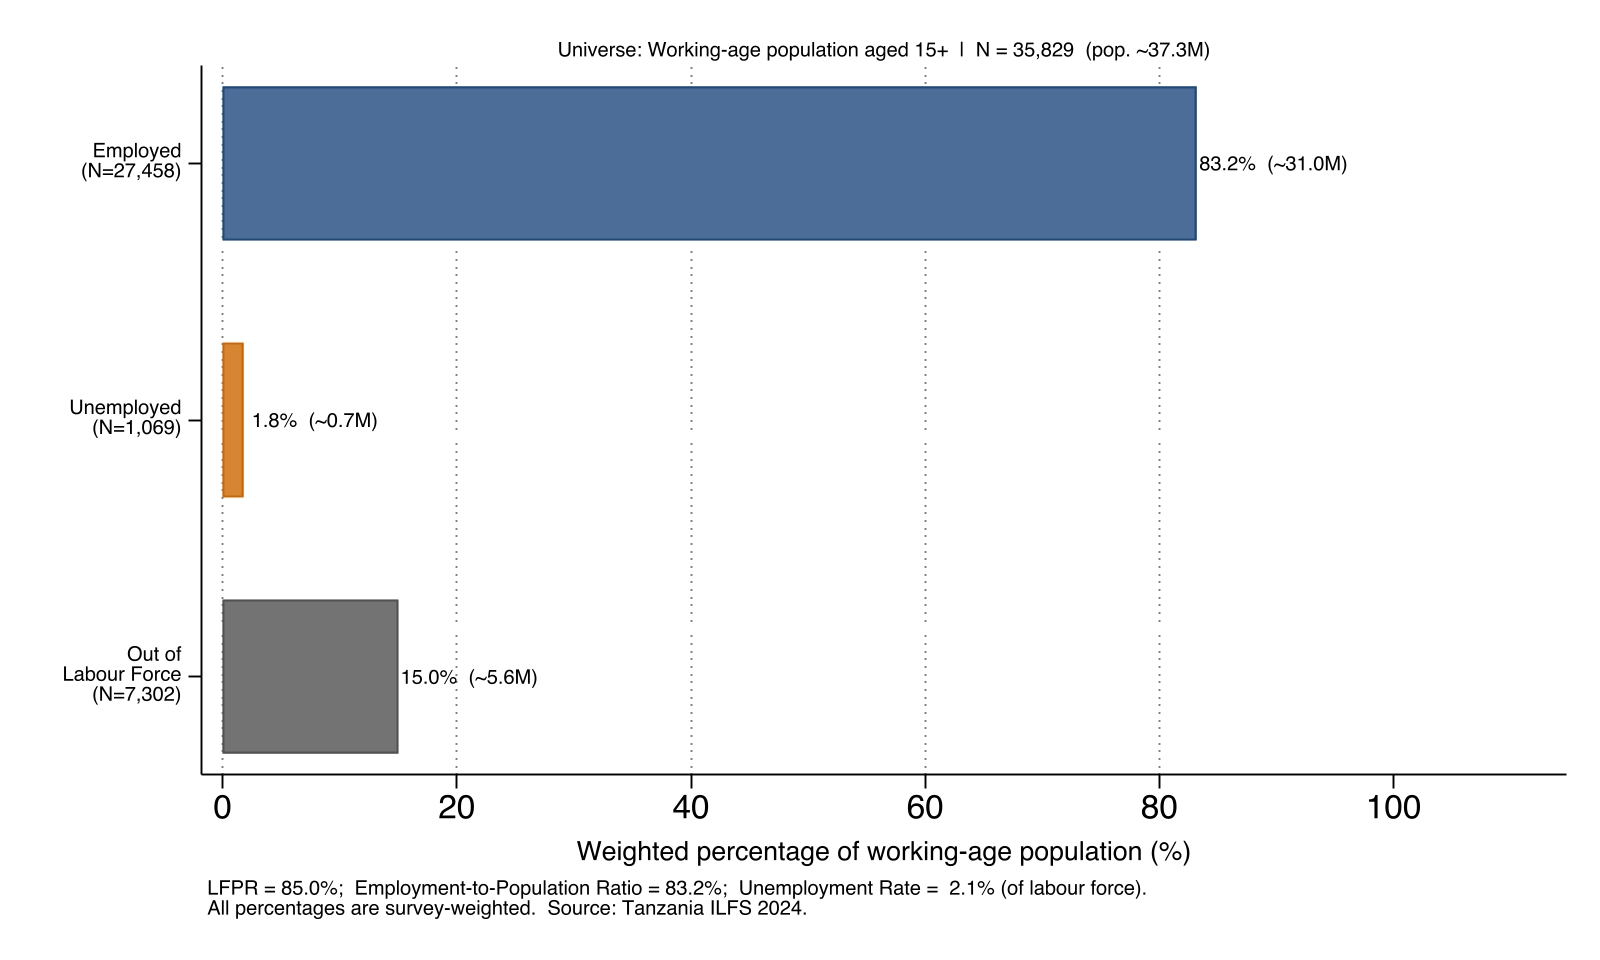
\includegraphics[width=0.85\textwidth]{figures/fig01_lfs_distribution.jpg}
  \caption{Distribution of labour force status, working-age population (aged 15+).}
  \label{fig:lfs_dist}
\end{figure}

Of the 35,829 respondents aged 15 and above, 27,458 were employed, 1,069 were unemployed, and 7,302 were out of the labour force in survey reference week (Table~\ref{tab:lfs_summary}). Weighted to the population, this corresponds to an employment rate of 83.2\%, an unemployment rate of 1.8\%, and a labour force participation rate of 85.0\%.

\begin{table}[H]
\centering
\caption{Labour force status summary (aged 15+).}
\label{tab:lfs_summary}
\begin{tabular}{lrrr}
\toprule
Category & $N$ (Unweighted) & Weighted \% & Pop.\ Estimate \\
\midrule
Employed            & 27,458 & 83.2\% & $\approx$ 31.0M \\
Unemployed          &  1,069 &  1.8\% & $\approx$  0.7M \\
Out of Labour Force &  7,302 & 15.0\% & $\approx$  5.6M \\
\midrule
Total (aged 15+)    & 35,829 & 100.0\% & $\approx$ 37.3M \\
\bottomrule
\end{tabular}

\smallskip
\footnotesize\textit{Note:} LFPR = 85.0\%; unemployment rate within the labour force = 2.1\%. $N$ = unweighted sample; \% = survey-weighted using WEIGHT.
\end{table}

\begin{figure}[H]
  \centering
  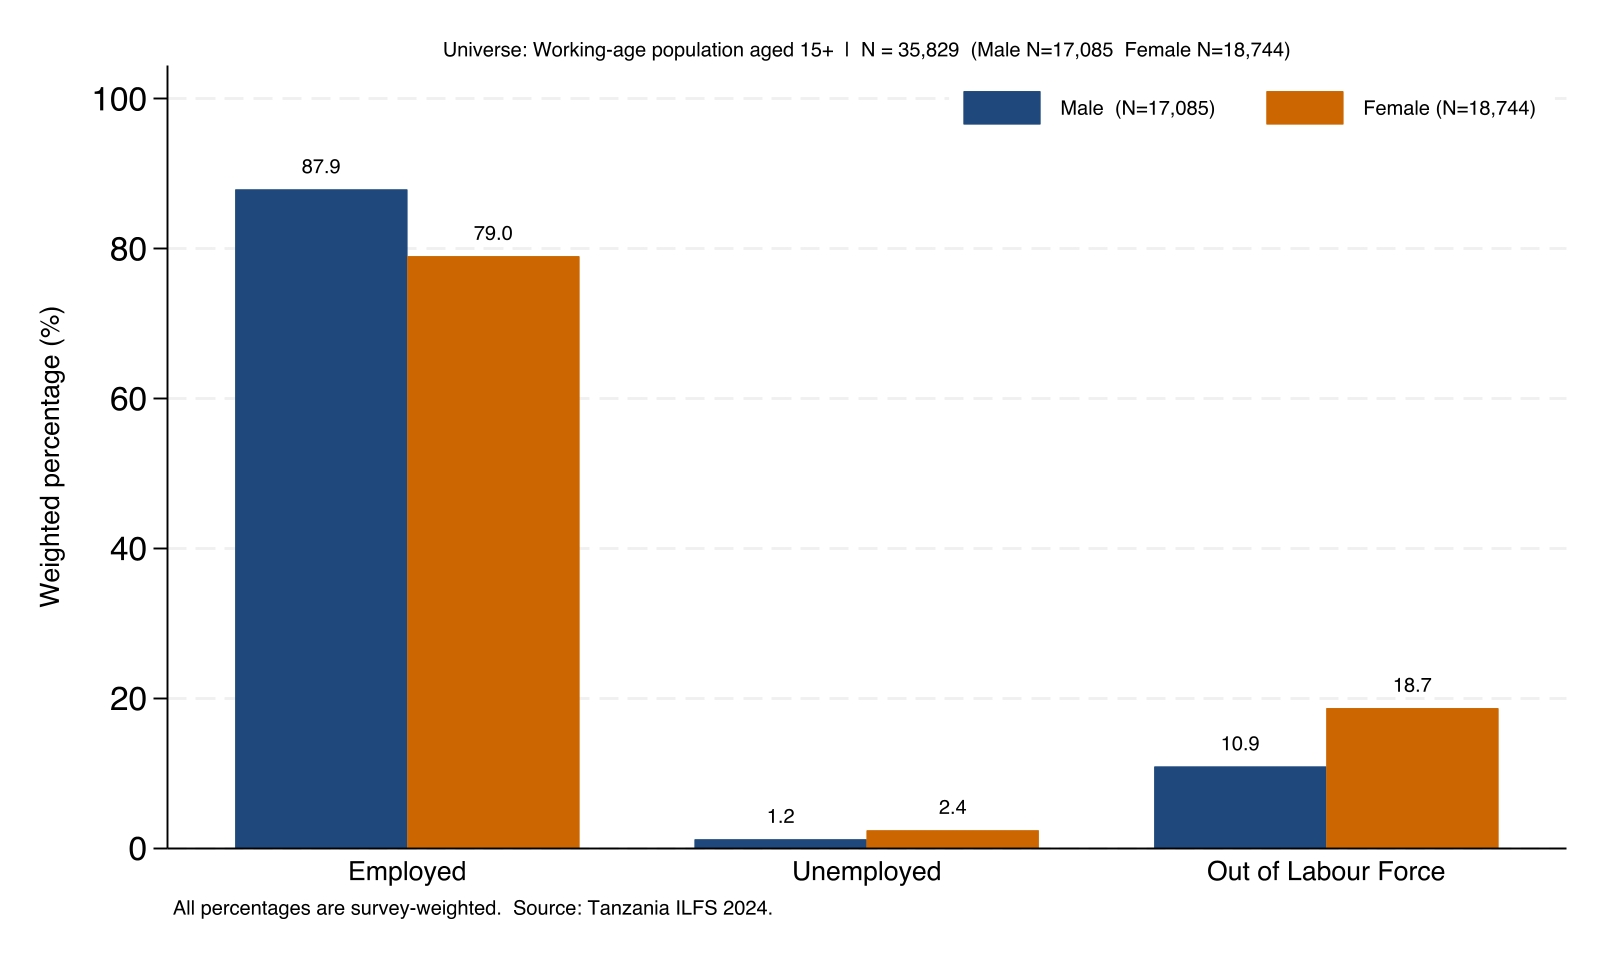
\includegraphics[width=0.85\textwidth]{figures/fig02_lfs_by_gender.jpg}
  \caption{Labour force status by gender.}
  \label{fig:lfs_gender}
\end{figure}

Disaggregation by gender (Figure~\ref{fig:lfs_gender}, Table~\ref{tab:lfs_gender}) reveals two distinct gaps. Female employment is 8.9 percentage points lower than male employment (79.0\% vs 87.9\%), and women are more than twice as likely to be unemployed within the labour force (2.9\% vs 1.3\%). The corresponding 7.8-point participation gap reflects mainly the higher female out-of-labour-force share (18.7\% vs 10.9\%); reasons for this difference are taken up in Section~\ref{sec:olf}.

\begin{table}[H]
\centering
\caption{Labour force status by gender.}
\label{tab:lfs_gender}
\begin{tabular}{lrrr}
\toprule
Indicator & Male & Female & Gap (F$-$M) \\
\midrule
$N$ (sample)               & 17,085  & 18,744  & --- \\
Employed (\%)              &  87.9\% &  79.0\% & $-$8.9 pp \\
Unemployed (\%)            &   1.2\% &   2.4\% & +1.2 pp \\
Out of Labour Force (\%)   &  10.9\% &  18.7\% & +7.8 pp \\
LFPR (\%)                  &  89.1\% &  81.3\% & $-$7.8 pp \\
Unemployment rate (\%)     &   1.3\% &   2.9\% & +1.6 pp \\
\bottomrule
\end{tabular}

\smallskip
\footnotesize\textit{Note:} Survey-weighted percentages. LFPR = labour force participation rate.
\end{table}


% ══════════════════════════════════════════════════════════
\section{Work Status Composition}
\label{sec:work_status}
% ══════════════════════════════════════════════════════════

\begin{figure}[H]
  \centering
  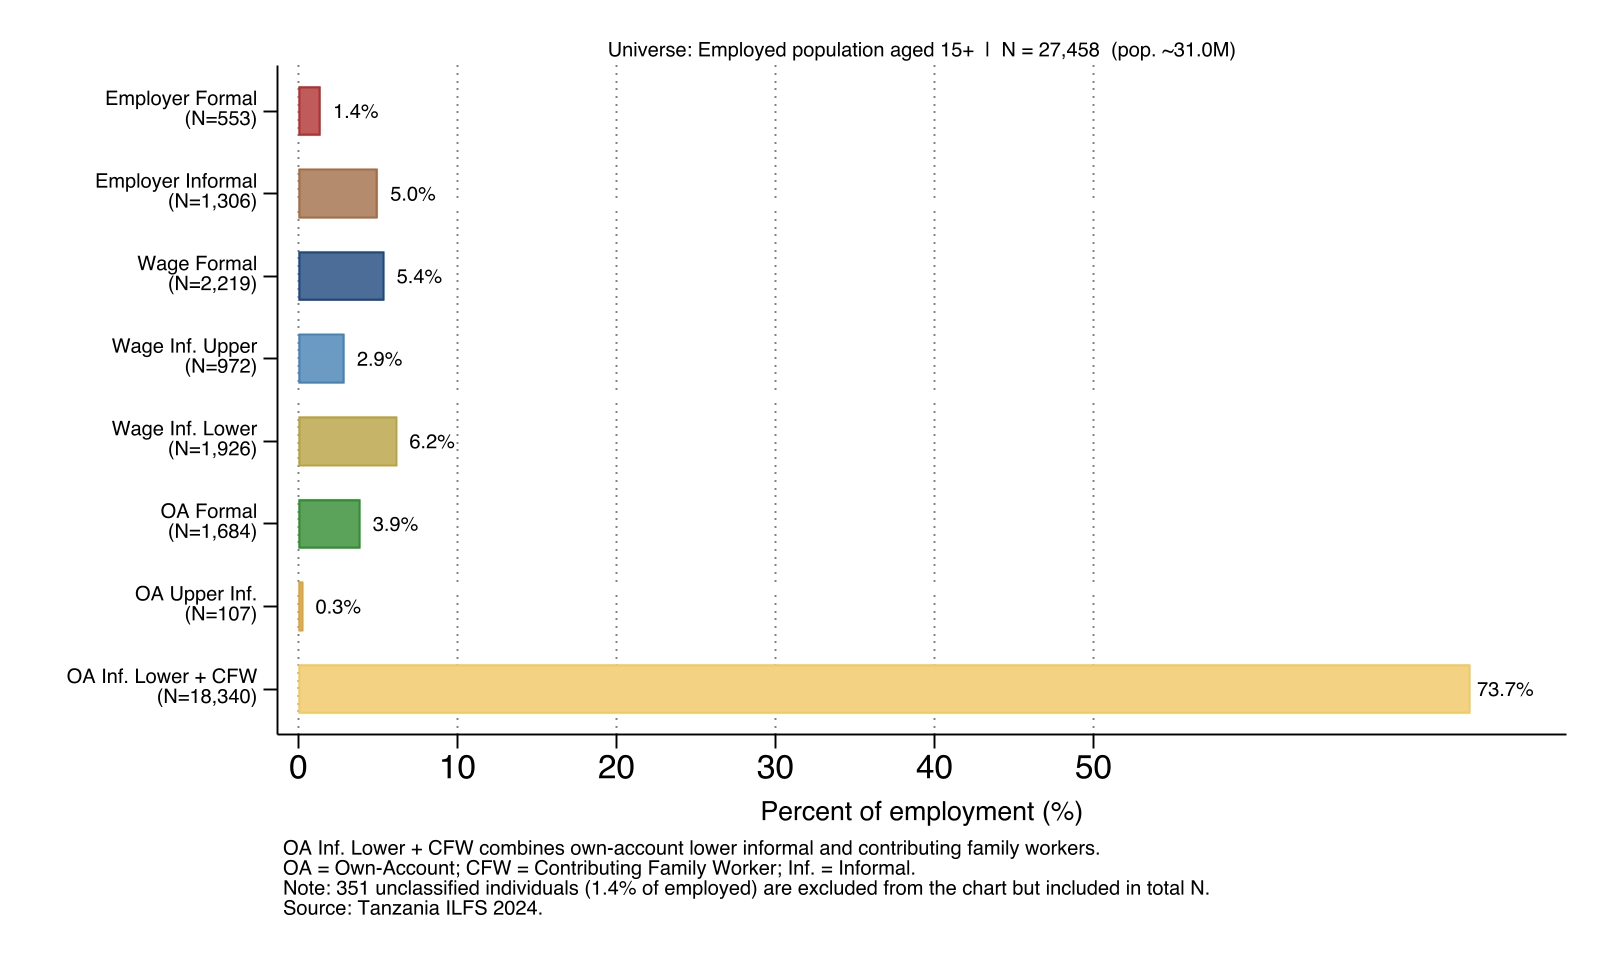
\includegraphics[width=0.85\textwidth]{figures/fig03_work_status_composition.jpg}
  \caption{Work status composition among employed respondents (eight-category display; OA lower informal and CFW combined).}
  \label{fig:ws_composition}
\end{figure}

Within the employed population, OA lower informal plus contributing family workers (CFW) account for 73.7\% of the total. Wage informal lower (6.2\%), wage formal (5.4\%) and the two employer categories combined (6.4\%) are the next largest segments (Figure~\ref{fig:ws_composition}, Table~\ref{tab:work_status}). Upper-tier informal categories---wage informal upper, OA upper informal---are small in aggregate, although they are useful for tracking better-paid informal work.

\begin{table}[H]
\centering
\caption{Work status classification (employed, aged 15+).}
\label{tab:work_status}
\small
\begin{tabularx}{\textwidth}{lrrX}
\toprule
Work Status & $N$ & Wt.\ \% & Definition \\
\midrule
Employer Formal        &   553  &  1.4\% & Self-employed with paid employees, registered business \\
Employer Informal Upper& 1,306  &  5.0\% & Self-employed with paid employees, unregistered business \\
Wage Formal            & 2,219  &  5.4\% & Paid employee with social security (Q34 codes 1 or 3) \\
Wage Informal Upper    &   972  &  2.9\% & Paid employee, no social security, TASCO 1--4 occupation \\
Wage Informal Lower    & 1,926  &  6.2\% & Paid employee, no social security, lower occupation; includes apprentices \\
OA Formal              & 1,684  &  3.9\% & Own-account worker with business registration (Q38A codes 1--5) \\
OA Upper Informal      &   107  &  0.3\% & Own-account, unregistered, TASCO 1--4 occupation \\
OA Informal Lower + CFW&18,340  & 73.7\% & OA lower informal plus contributing family workers (display merge) \\
Unclassified           &   351  &  1.4\% & Employed with missing status-in-employment information \\
\bottomrule
\end{tabularx}

\smallskip
\footnotesize\textit{Note:} OA = Own-Account; CFW = Contributing Family Worker. The analytical pipeline constructs a full ten-category work status variable; the figures use an eight-category display by merging OA lower informal and CFW.
\end{table}

\subsection{Gender composition of work status}

Every wage and employer category has a higher male than female share, while OA lower informal and CFW account for 81.4\% of female employment against 66.0\% of male employment (Figure~\ref{fig:gender_gap}, Table~\ref{tab:ws_gender}). Wage informal lower is 3.7 points more common among men, and employer informal upper 3.5 points more common; wage formal accounts for 6.9\% of men's jobs and 3.8\% of women's. Side-by-side bars (Figure~\ref{fig:ws_by_gender}) and the gendered pie/stacked-bar pair (Figure~\ref{fig:ws_pie}) make the same point in alternative formats; the simplest summary is that women are far more concentrated in the lowest-tier residual category.

\begin{figure}[H]
  \centering
  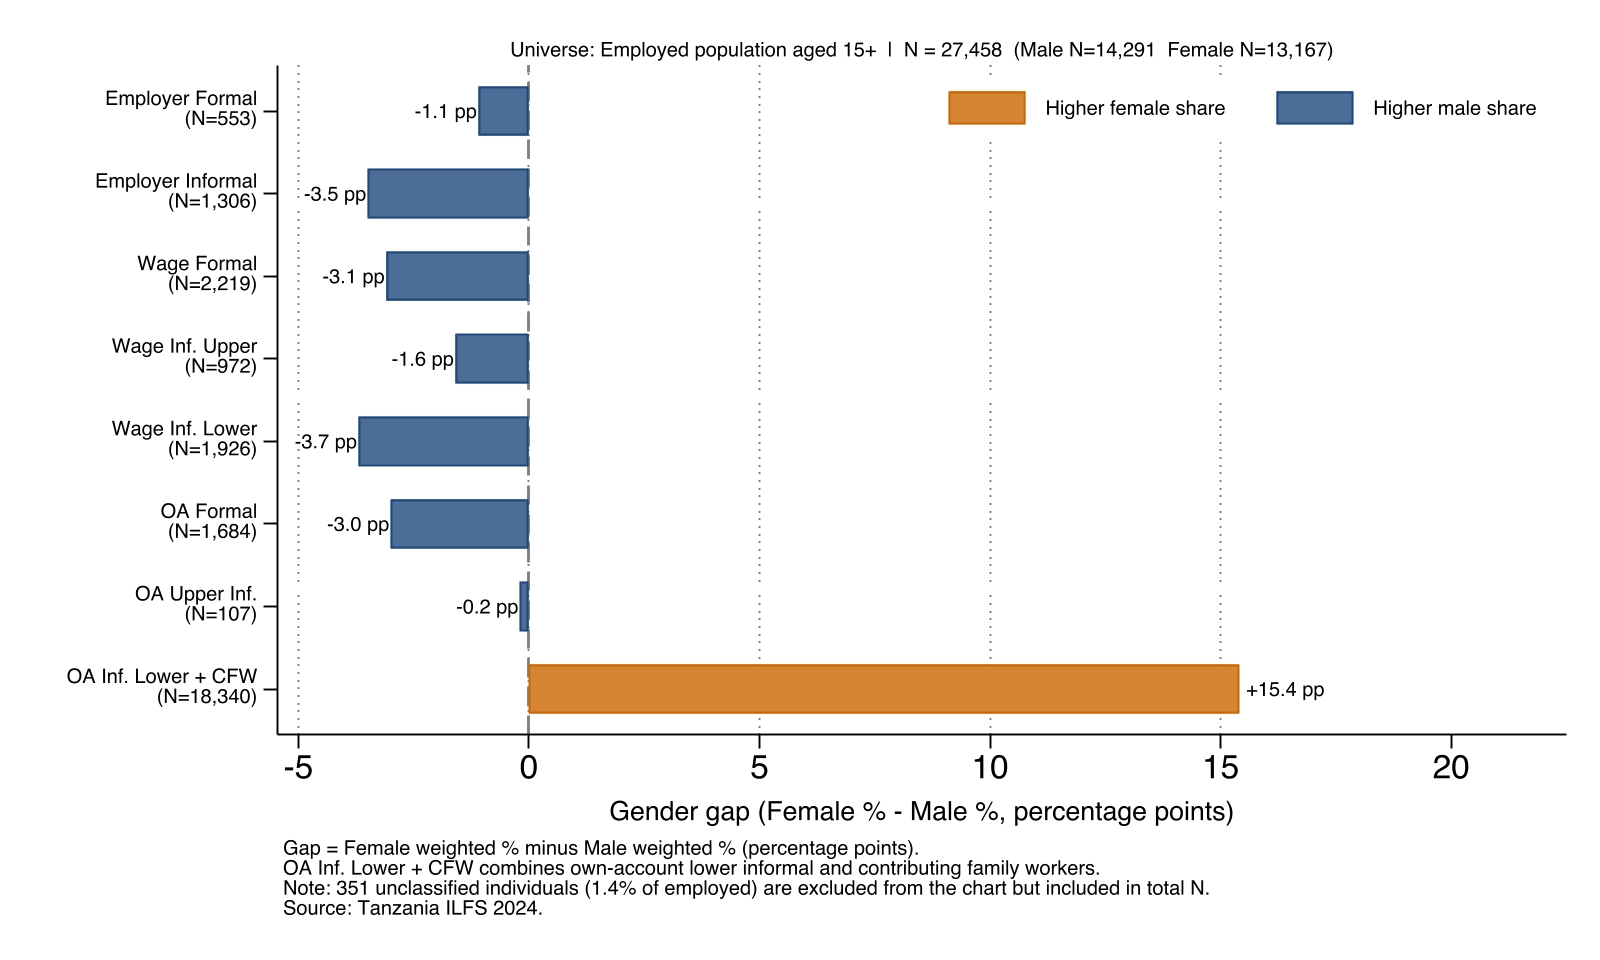
\includegraphics[width=0.85\textwidth]{figures/fig04_gender_gap_work_status.jpg}
  \caption{Gender gap (female \% $-$ male \%, in percentage points) for each work status category.}
  \label{fig:gender_gap}
\end{figure}

\begin{figure}[H]
  \centering
  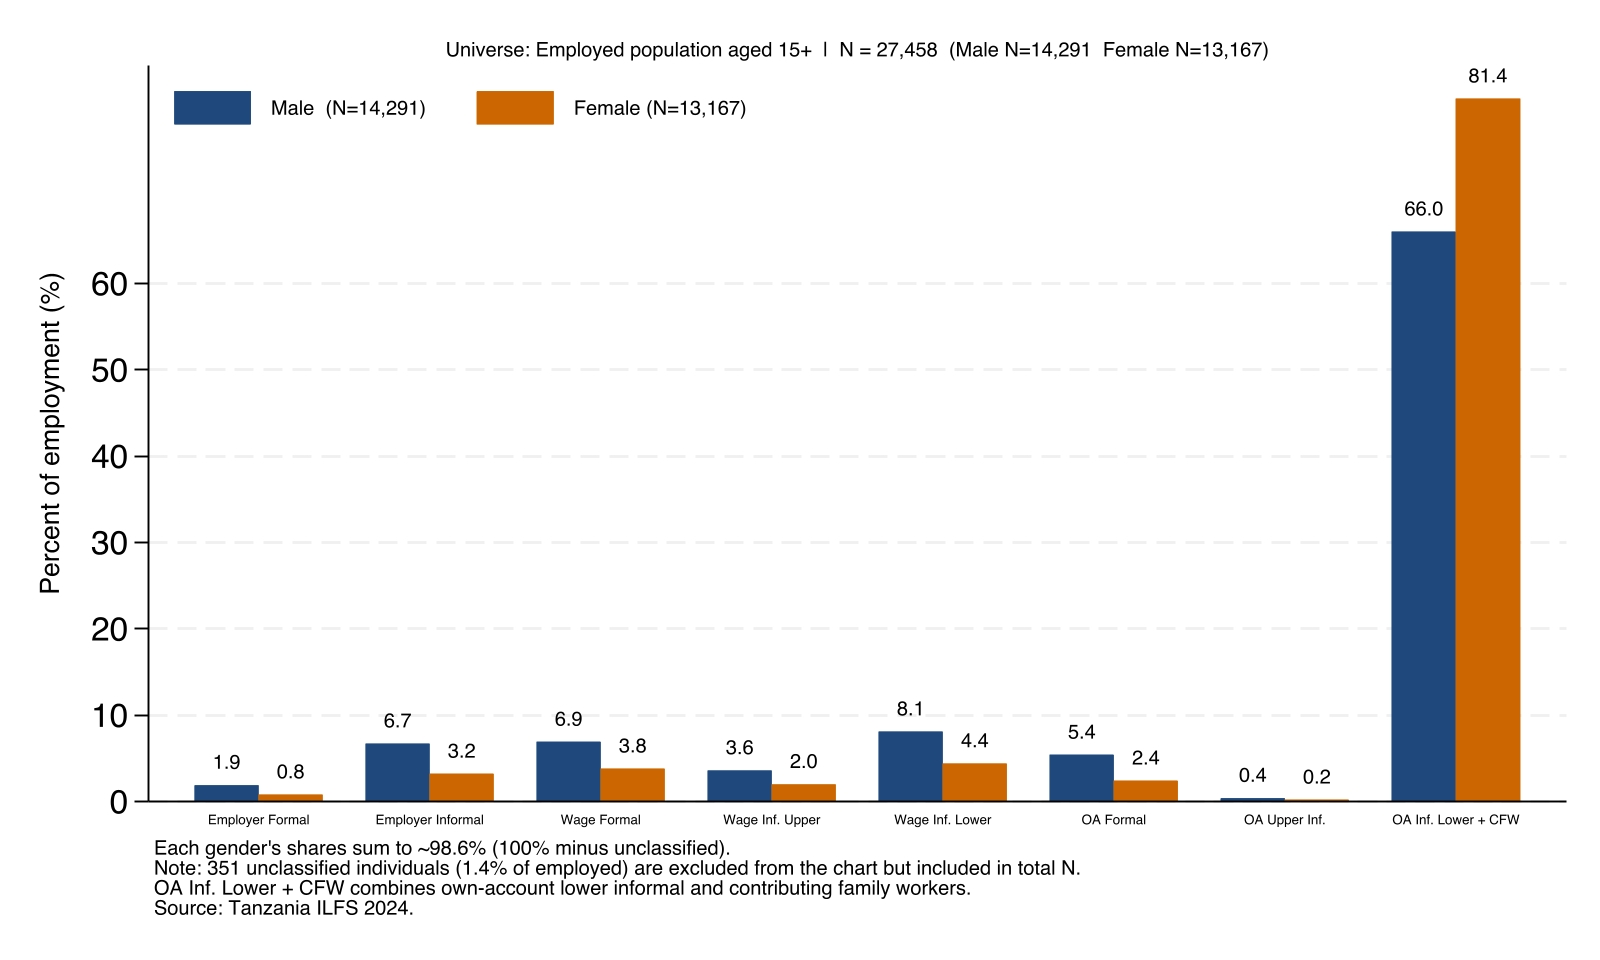
\includegraphics[width=0.85\textwidth]{figures/fig05_work_status_by_gender.jpg}
  \caption{Work status breakdown by gender (side-by-side bars).}
  \label{fig:ws_by_gender}
\end{figure}

\begin{table}[H]
\centering
\caption{Work status by gender (employed, aged 15+).}
\label{tab:ws_gender}
\small
\begin{tabular}{lrrrrrr}
\toprule
Work Status & Male $N$ & Male \% & Female $N$ & Female \% & Gap (pp) \\
\midrule
Employer Formal      &   412 &  1.9\% &   141 &  0.8\% & $-$1.2 \\
Employer Inf.\ Upper &   916 &  6.7\% &   390 &  3.2\% & $-$3.5 \\
Wage Formal          & 1,402 &  6.9\% &   817 &  3.8\% & $-$3.1 \\
Wage Inf.\ Upper     &   594 &  3.6\% &   378 &  2.0\% & $-$1.6 \\
Wage Inf.\ Lower     & 1,244 &  8.1\% &   682 &  4.4\% & $-$3.7 \\
OA Formal            & 1,287 &  5.4\% &   397 &  2.4\% & $-$3.0 \\
OA Upper Inf.        &    73 &  0.4\% &    34 &  0.2\% & $-$0.2 \\
OA Inf.\ Lower + CFW & 8,248 & 66.0\% & 10,092 & 81.4\% & +15.4 \\
\bottomrule
\end{tabular}

\smallskip
\footnotesize\textit{Note:} \% = survey-weighted share within each gender's employed total. Gap = female \% $-$ male \%.
\end{table}

\begin{figure}[H]
  \centering
  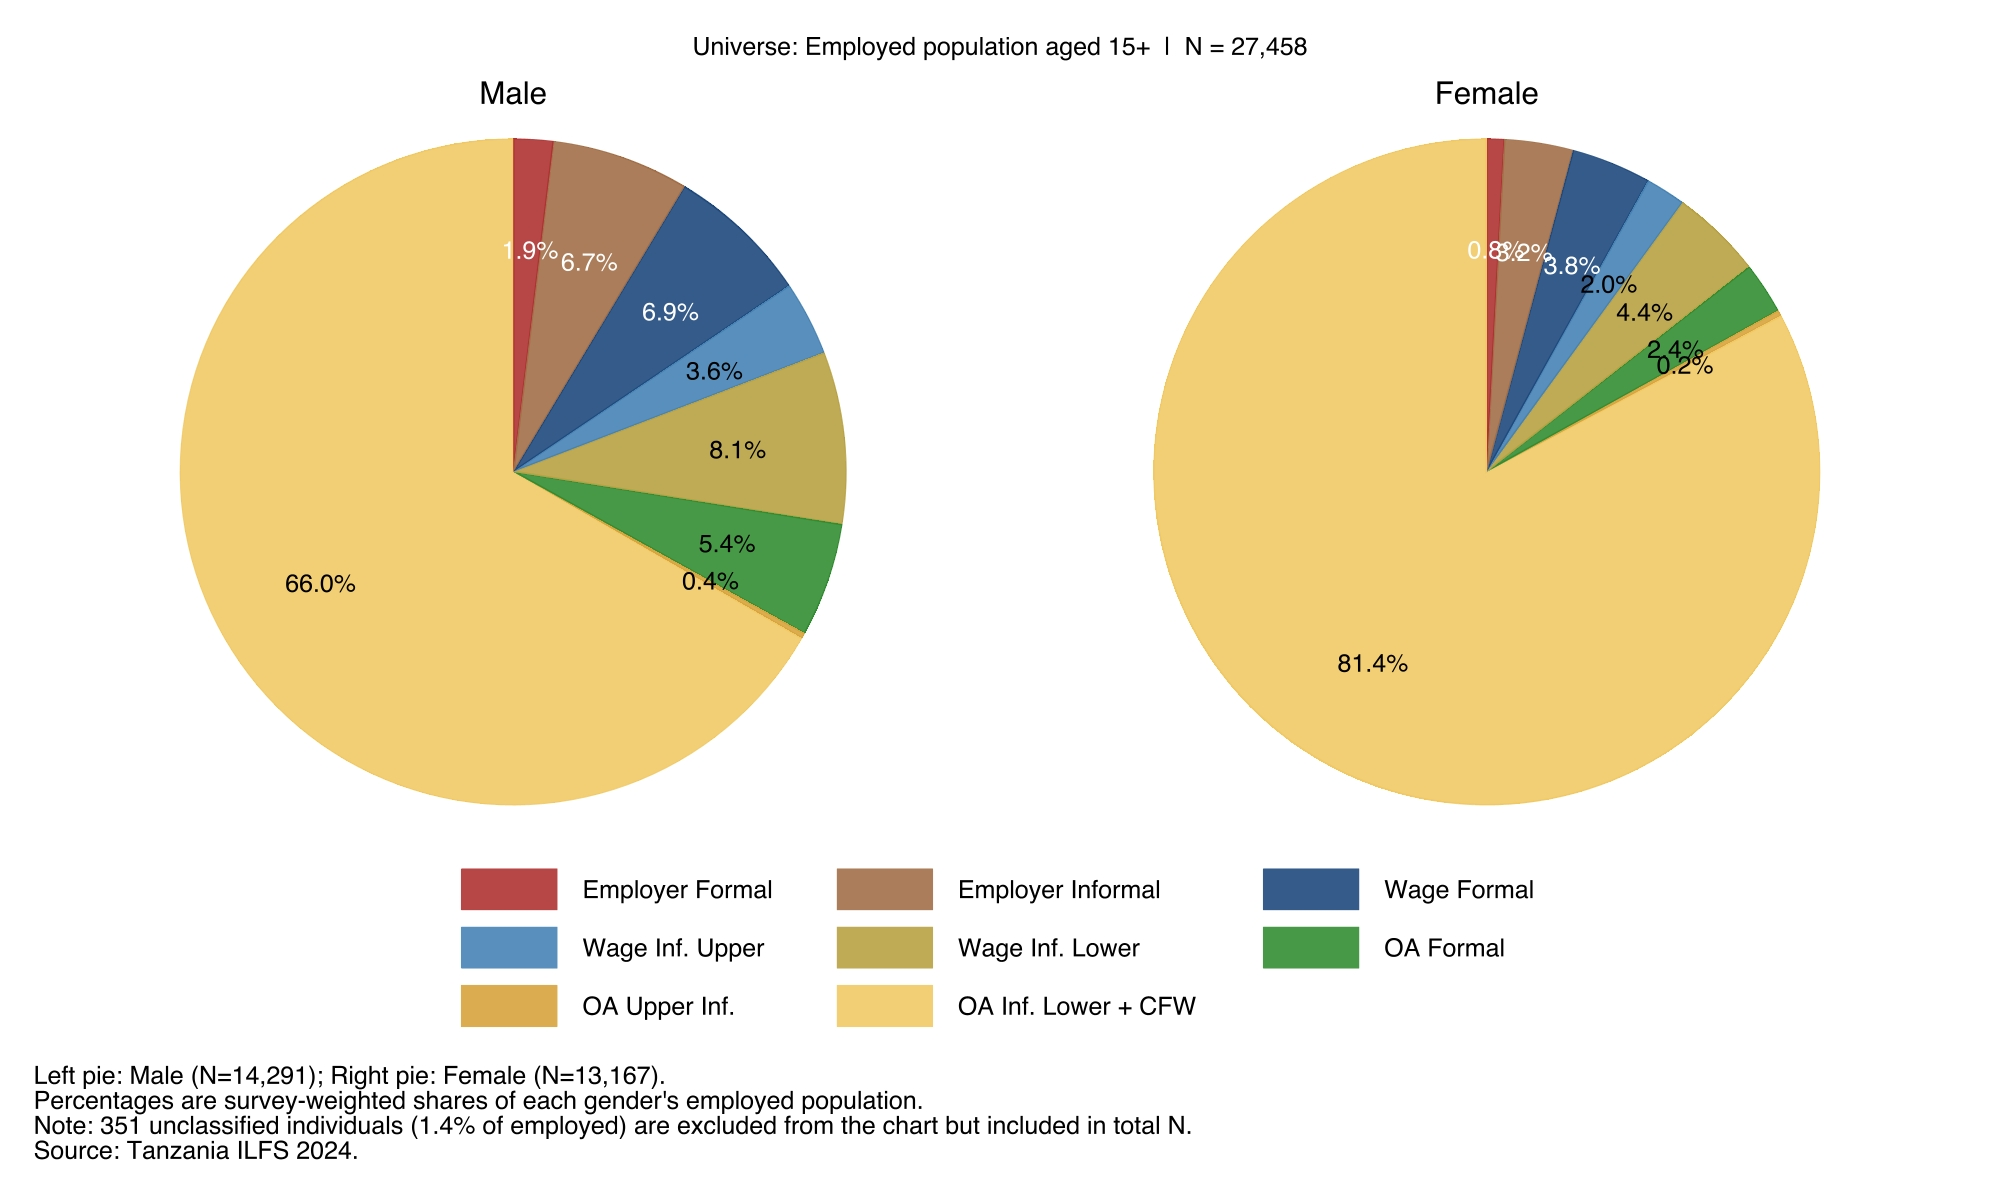
\includegraphics[width=0.85\textwidth]{figures/fig11_ws_pie_by_gender.jpg}
  \caption{Work status composition pie charts by gender.}
  \label{fig:ws_pie}
\end{figure}

\begin{figure}[H]
  \centering
  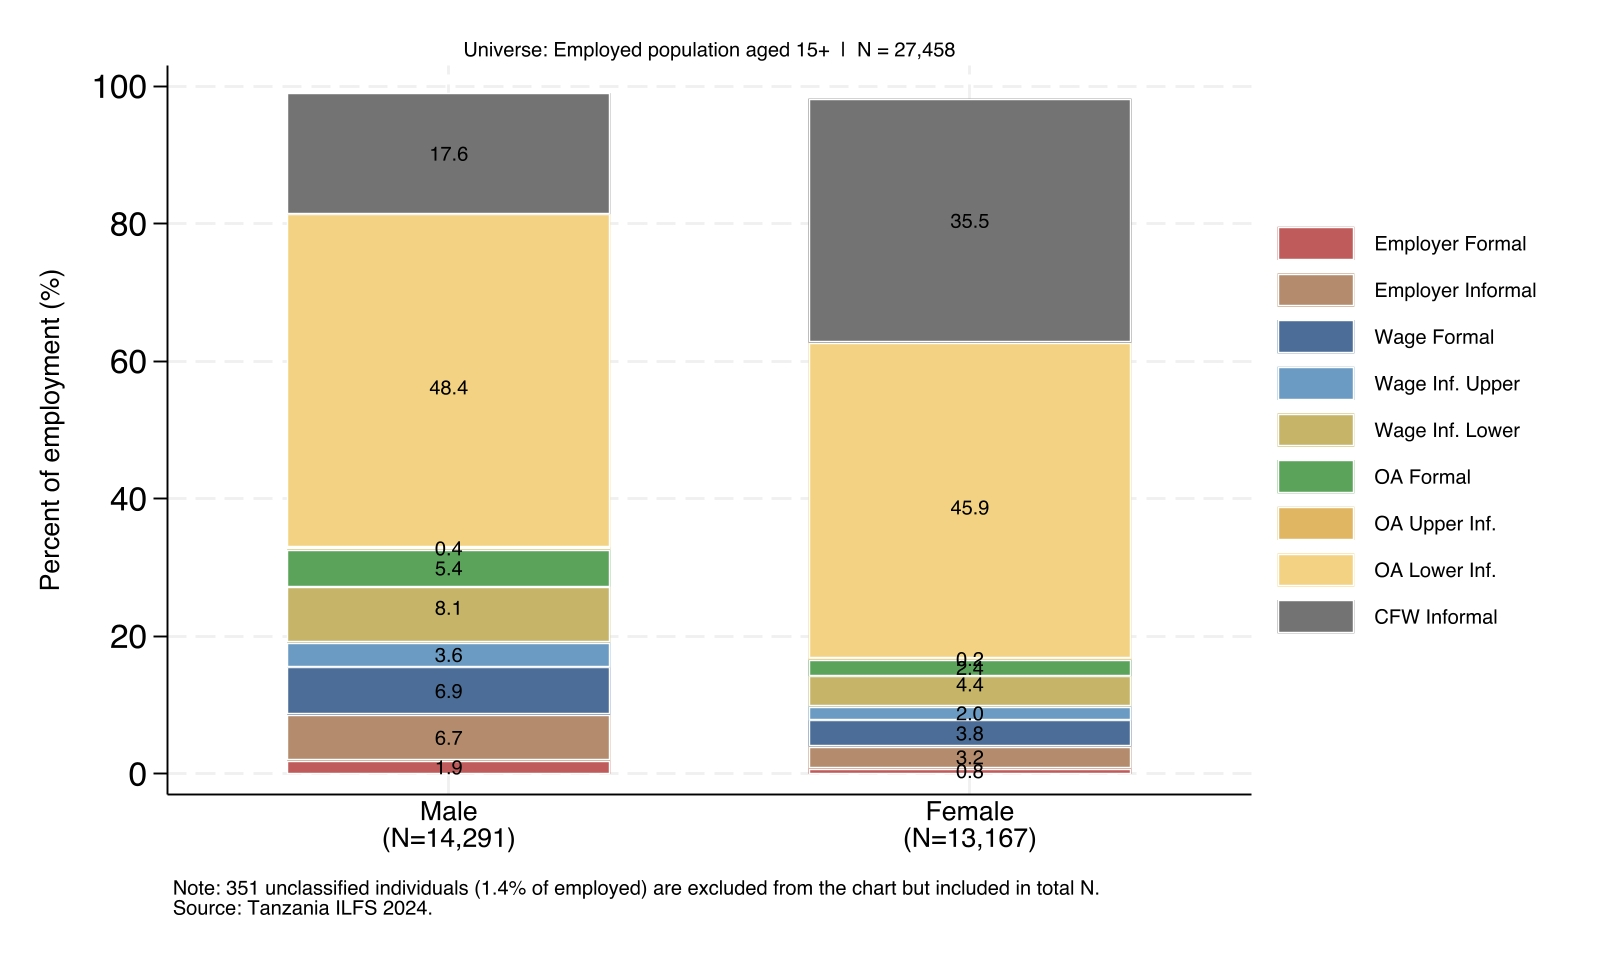
\includegraphics[width=0.85\textwidth]{figures/fig12_ws_stacked_by_gender.jpg}
  \caption{Work status, 100\% stacked bars by gender.}
  \label{fig:ws_stacked}
\end{figure}


% ══════════════════════════════════════════════════════════
\section{Education}
\label{sec:education}
% ══════════════════════════════════════════════════════════

\subsection{Education by gender}

Primary education accounts for the majority of employed workers in both genders (62.0\% of men and 60.1\% of women), but the tails differ (Figure~\ref{fig:educ_gender}, Table~\ref{tab:educ_gender}). Women are about twice as likely to have no formal education (16.0\% vs 8.3\%), and less likely to have completed O-Level (18.5\% vs 22.2\%) or higher education (3.7\% vs 5.3\%).

\begin{figure}[H]
  \centering
  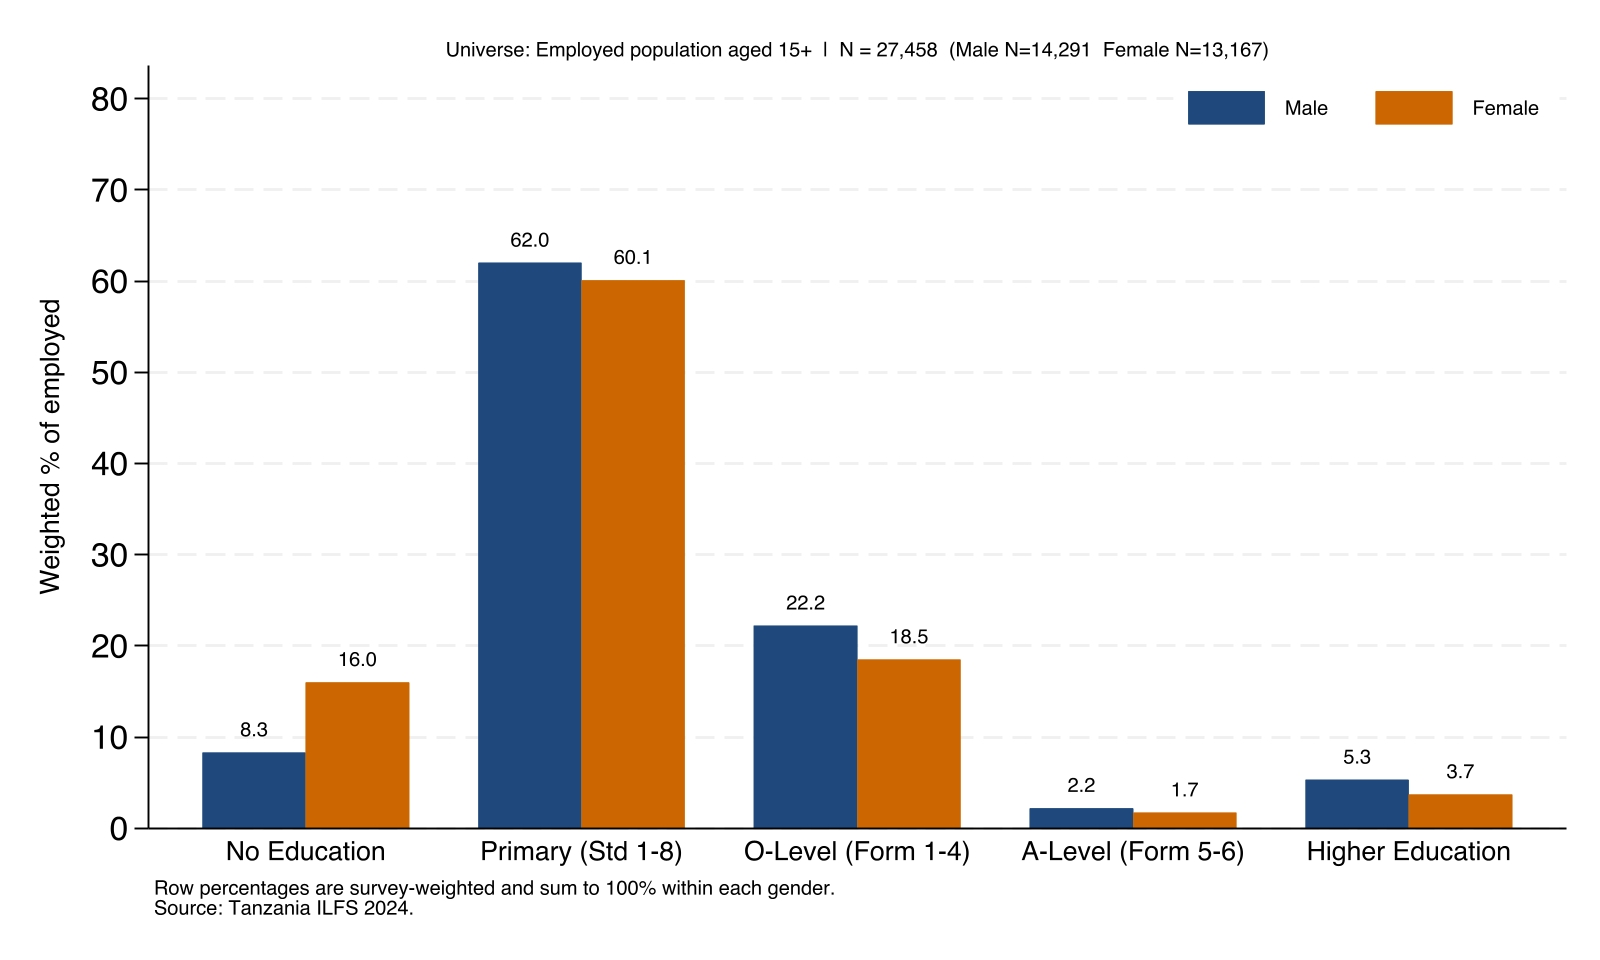
\includegraphics[width=0.85\textwidth]{figures/fig06_education_by_gender.jpg}
  \caption{Education distribution of employed workers by gender.}
  \label{fig:educ_gender}
\end{figure}

\begin{table}[H]
\centering
\caption{Education level by gender (employed, aged 15+).}
\label{tab:educ_gender}
\begin{tabular}{lrrr}
\toprule
Education Level & Male \% & Female \% & Gap (F$-$M, pp) \\
\midrule
No Education          &  8.3\% & 16.0\% & +7.7 \\
Primary (Std 1--8)    & 62.0\% & 60.1\% & $-$1.9 \\
O-Level (Form 1--4)   & 22.2\% & 18.5\% & $-$3.7 \\
A-Level (Form 5--6)   &  2.2\% &  1.7\% & $-$0.5 \\
Higher Education      &  5.3\% &  3.7\% & $-$1.6 \\
\bottomrule
\end{tabular}

\smallskip
\footnotesize\textit{Note:} Survey-weighted; rows sum to 100\% within gender (excluding missing).
\end{table}

\subsection{Education by work status}

Education profiles vary sharply across work statuses (Figure~\ref{fig:educ_ws}). Wage formal workers carry the highest share of O-Level and above qualifications, while OA lower informal and CFW workers are concentrated at primary or below. The same pattern persists among youth (Figure~\ref{fig:educ_ws_youth}), which suggests that education is sorting workers into segments early in their careers rather than only over time.

\begin{figure}[H]
  \centering
  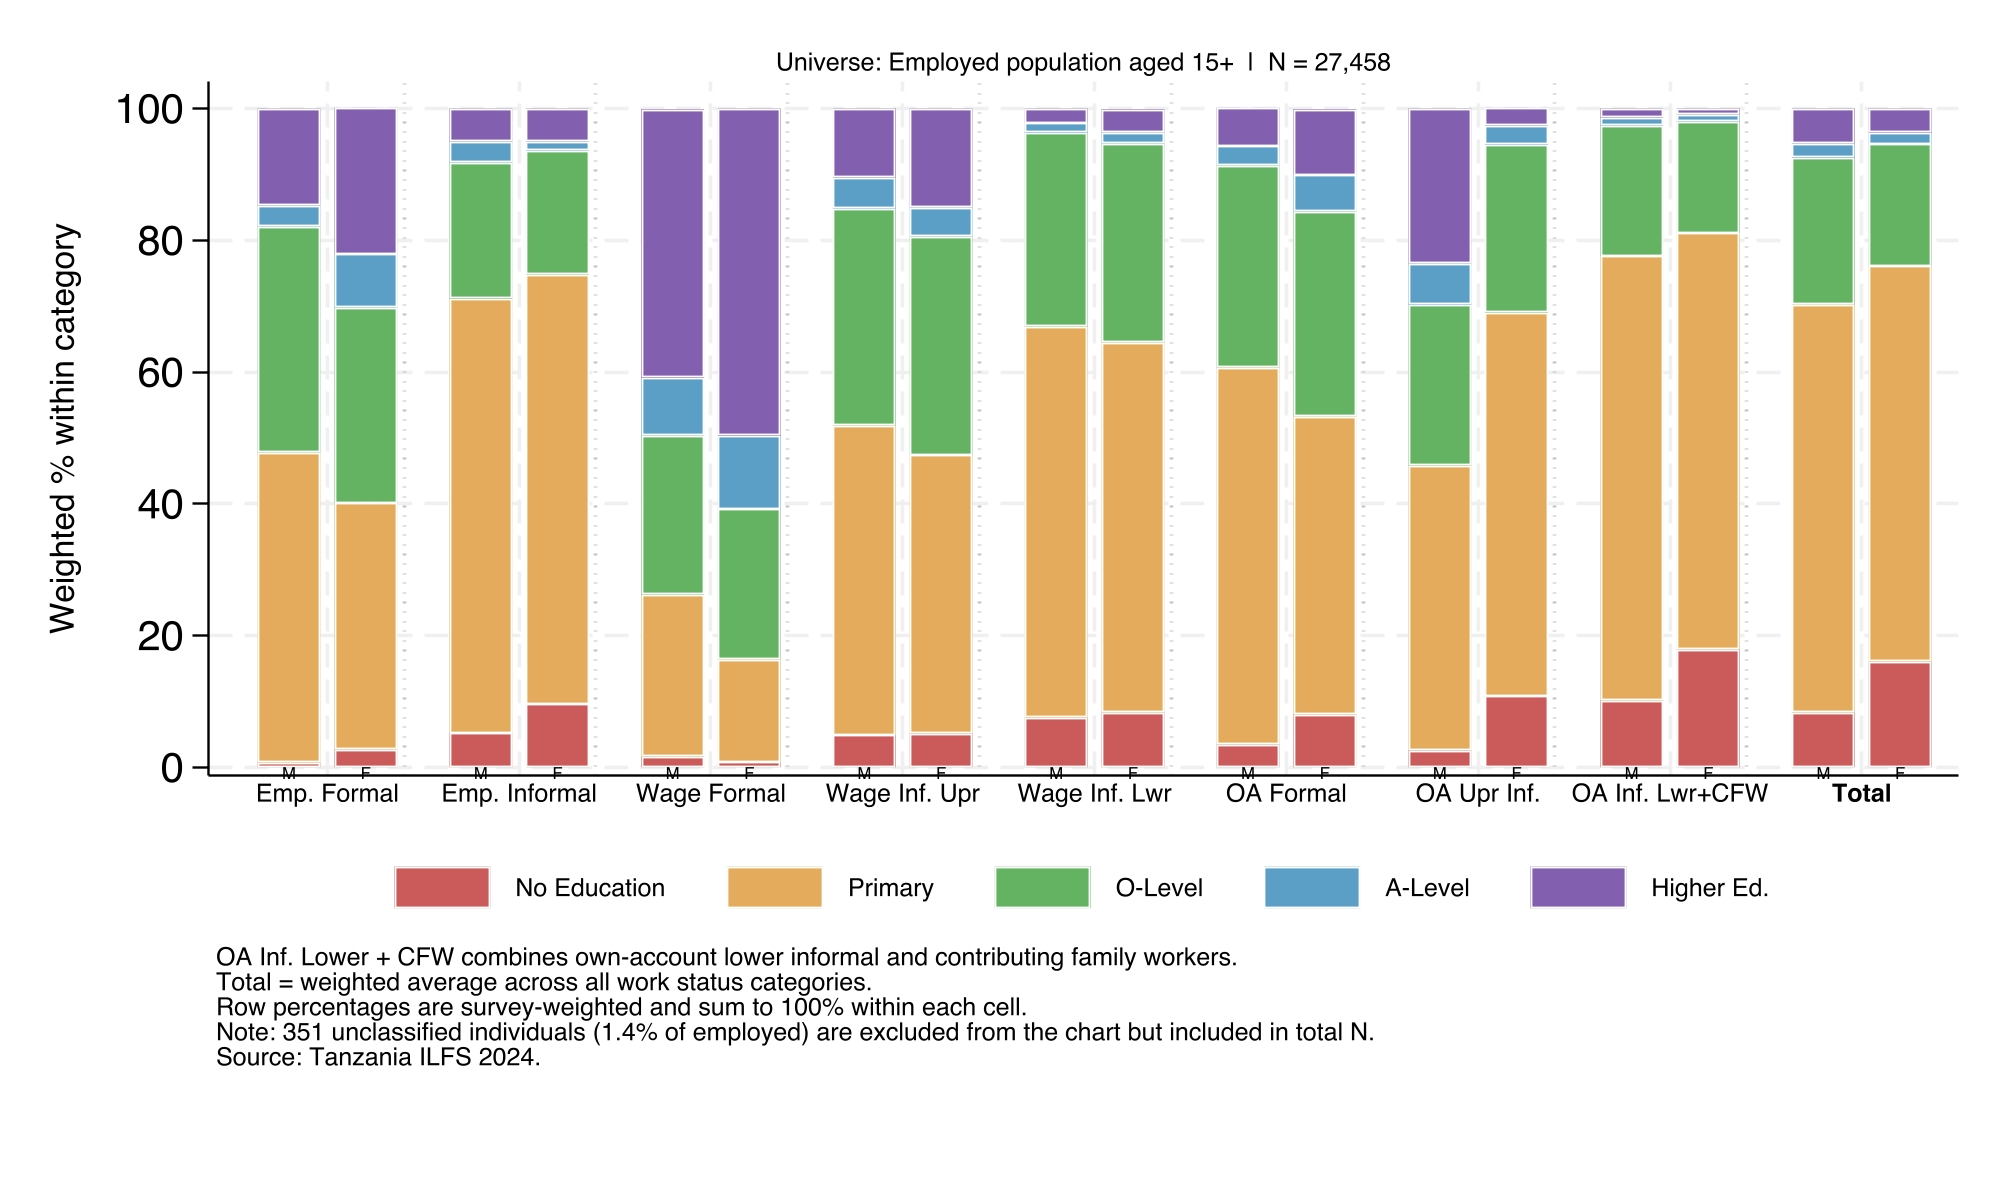
\includegraphics[width=\textwidth]{figures/fig07_education_by_ws_gender.jpg}
  \caption{Education profile within each work status category, by gender.}
  \label{fig:educ_ws}
\end{figure}

\begin{figure}[H]
  \centering
  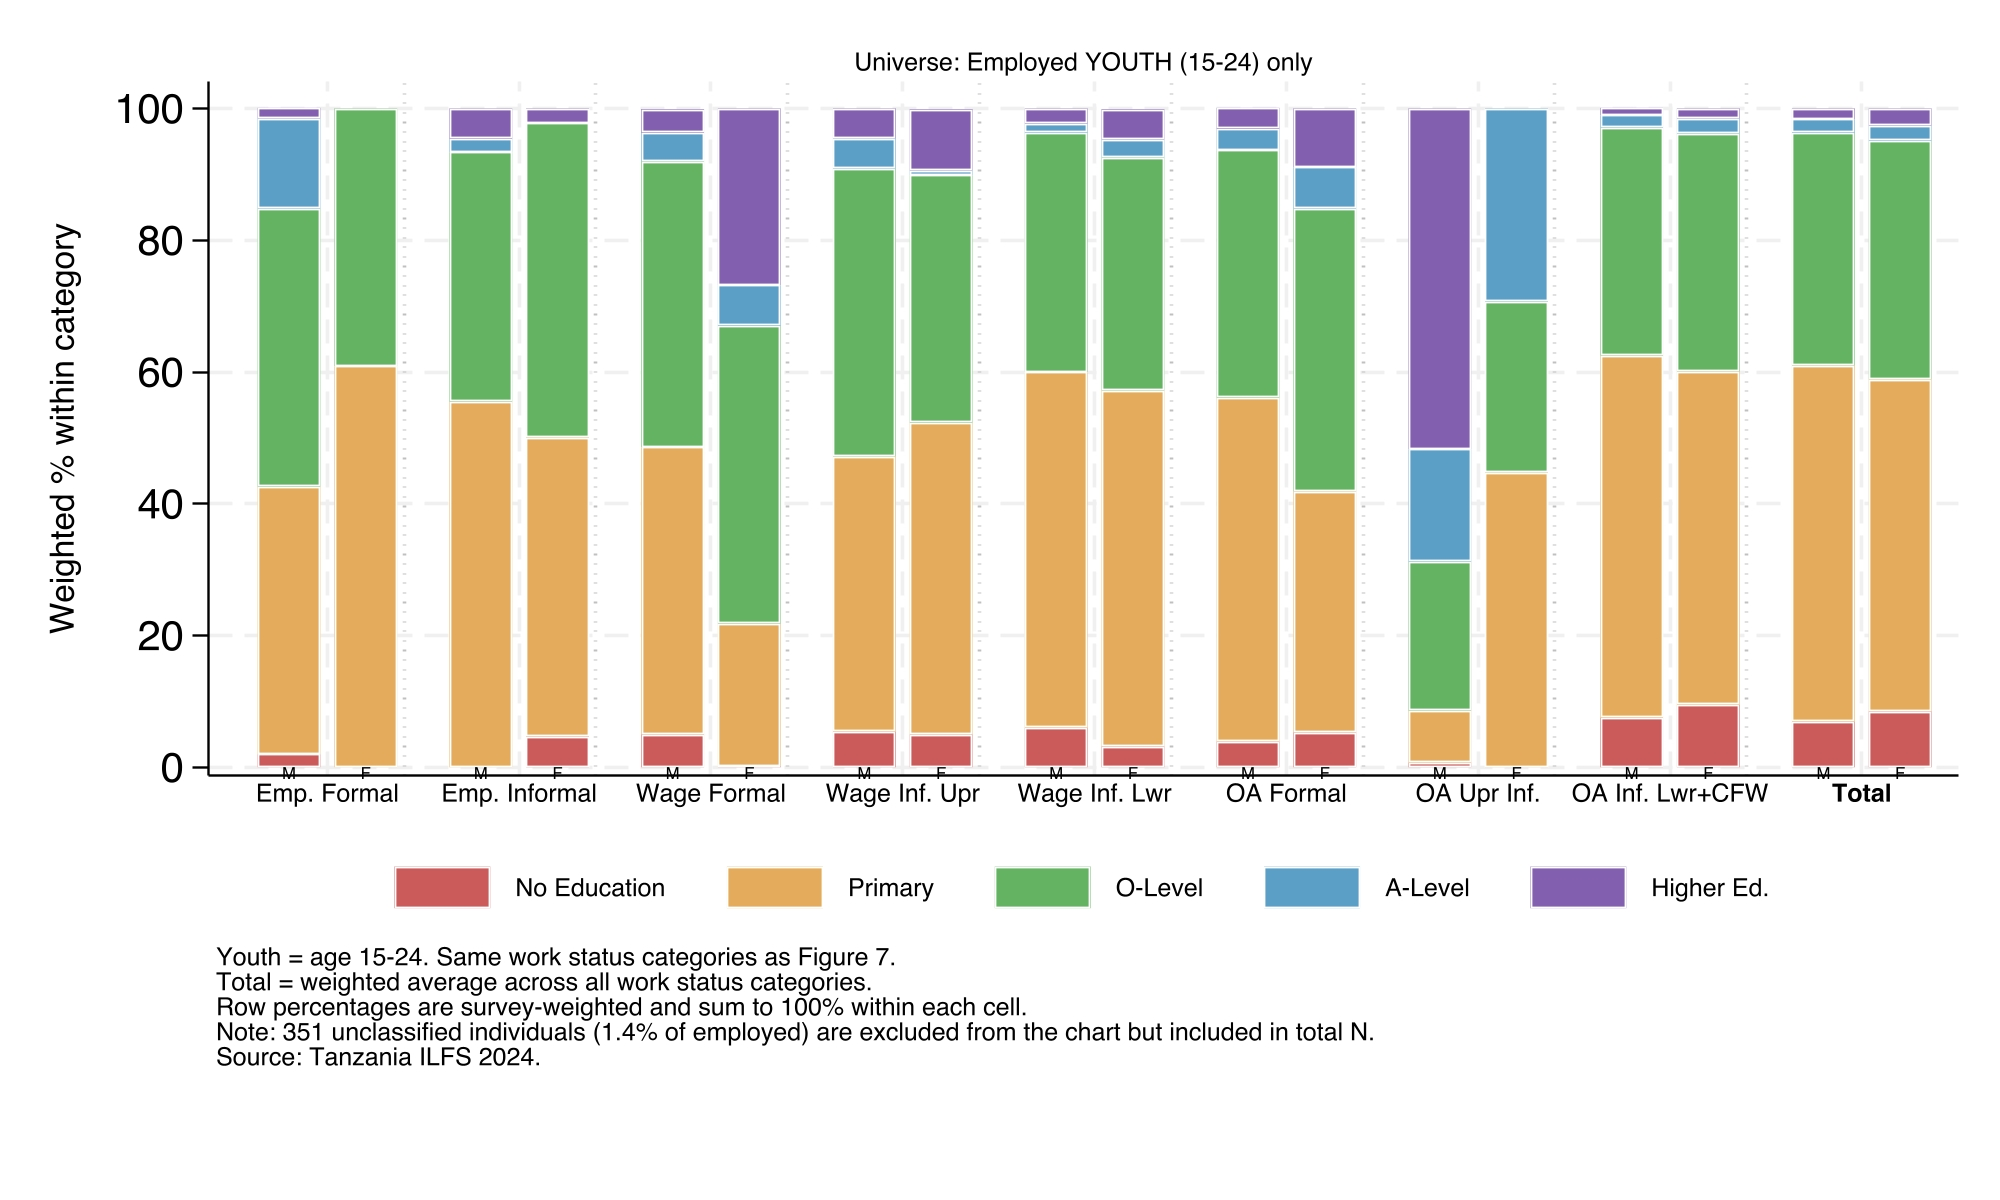
\includegraphics[width=\textwidth]{figures/fig07b_education_by_ws_gender_youth.jpg}
  \caption{Education profile by work status and gender, youth (15--24).}
  \label{fig:educ_ws_youth}
\end{figure}

\subsection{Education in higher-tier categories}
\label{sec:educ_formal}

Restricting attention to the three higher-tier work statuses (wage formal, wage informal upper, OA upper informal) sharpens the picture (Figure~\ref{fig:educ_formal}, Table~\ref{tab:educ_formal}). Among wage formal workers, women hold a higher share of higher-education qualifications than men (49.7\% vs 40.8\%), consistent with women facing a more selective entry threshold for formal jobs. The wage informal upper category shows the same direction at smaller magnitude. The picture inverts for OA upper informal: 23.5\% of men hold higher-education qualifications, against 2.7\% of women, with women instead concentrated in primary education (58.2\%). Sample sizes for OA upper informal are small ($N=73$ men, 34 women), so the magnitude should be read with care; the direction is consistent with occupational segregation operating even within the upper-tier informal category.

\begin{figure}[H]
  \centering
  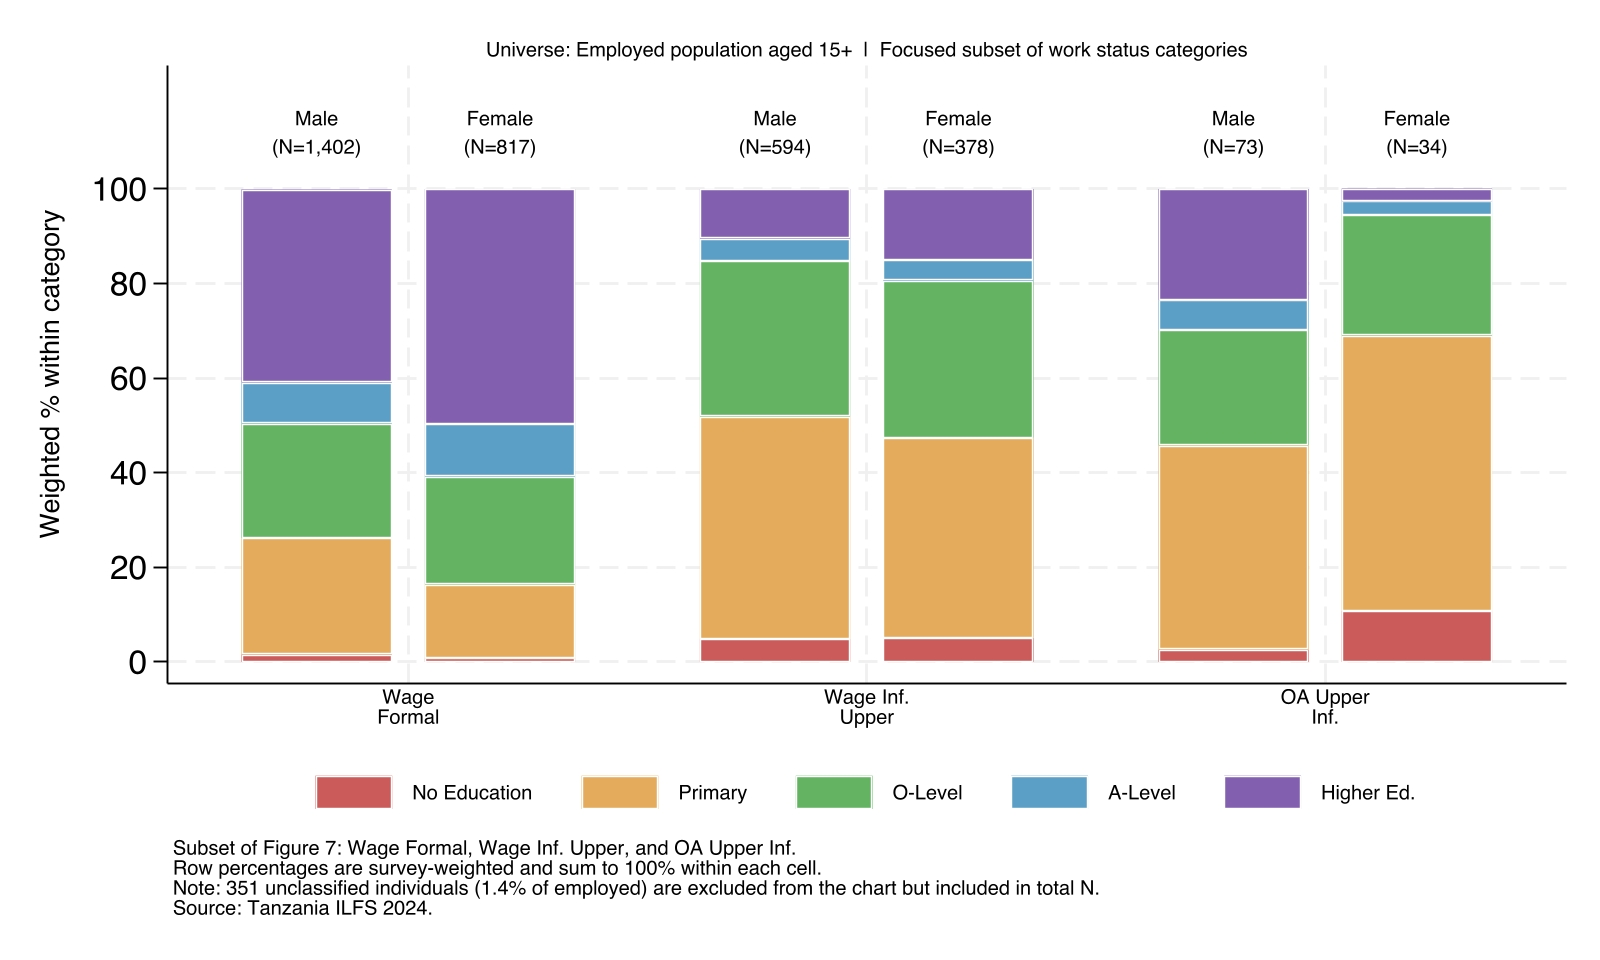
\includegraphics[width=0.85\textwidth]{figures/fig15_education_formal_upper_inf.jpg}
  \caption{Education profiles for the three higher-tier work status categories, by gender.}
  \label{fig:educ_formal}
\end{figure}

\begin{table}[H]
\centering
\caption{Education by gender for higher-tier work status categories.}
\label{tab:educ_formal}
\small
\begin{tabular}{llrrrrr}
\toprule
Work Status & Gender & $N$ & No Ed. & Primary & O-Level & Higher Ed. \\
\midrule
Wage Formal      & Male   & 1,402 &  1.6\% & 24.6\% & 24.2\% & 40.8\% \\
Wage Formal      & Female &   817 &  0.8\% & 15.6\% & 22.8\% & 49.7\% \\
\addlinespace
Wage Inf.\ Upper & Male   &   594 &  4.9\% & 47.0\% & 32.9\% & 10.5\% \\
Wage Inf.\ Upper & Female &   378 &  5.1\% & 42.3\% & 33.2\% & 15.0\% \\
\addlinespace
OA Upper Inf.    & Male   &    73 &  2.6\% & 43.2\% & 24.4\% & 23.5\% \\
OA Upper Inf.    & Female &    34 & 10.8\% & 58.2\% & 25.5\% &  2.7\% \\
\bottomrule
\end{tabular}

\smallskip
\footnotesize\textit{Note:} Row percentages, survey-weighted. A-Level omitted for space; rows sum to 100\%. OA upper informal sample is small.
\end{table}


% ══════════════════════════════════════════════════════════
\section{Youth (15--24) Employment}
\label{sec:youth}
% ══════════════════════════════════════════════════════════

\begin{figure}[H]
  \centering
  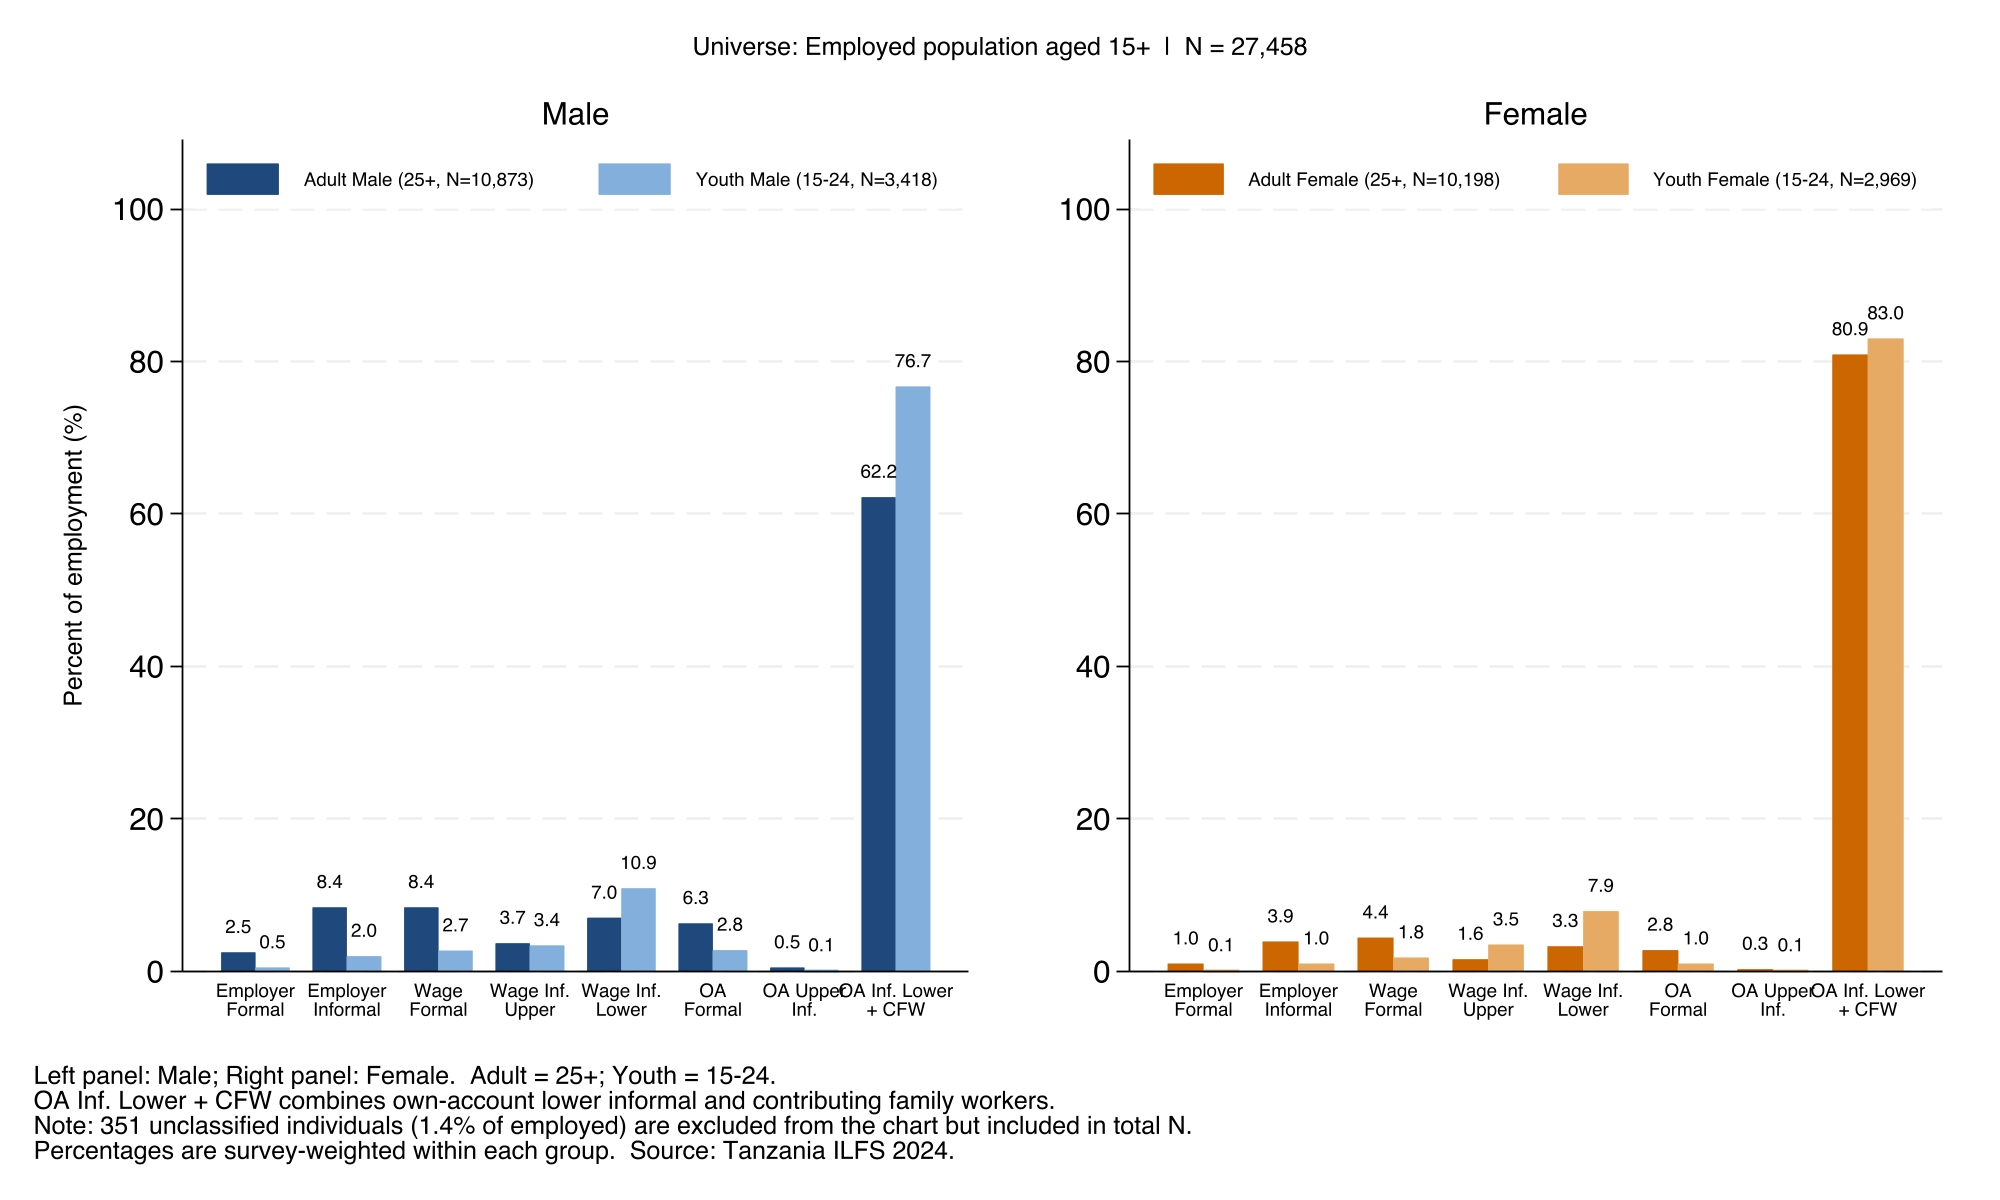
\includegraphics[width=0.85\textwidth]{figures/fig08_work_status_youth_gender.jpg}
  \caption{Work status: youth (15--24) versus adults (25+) by gender.}
  \label{fig:youth}
\end{figure}

\begin{figure}[H]
  \centering
  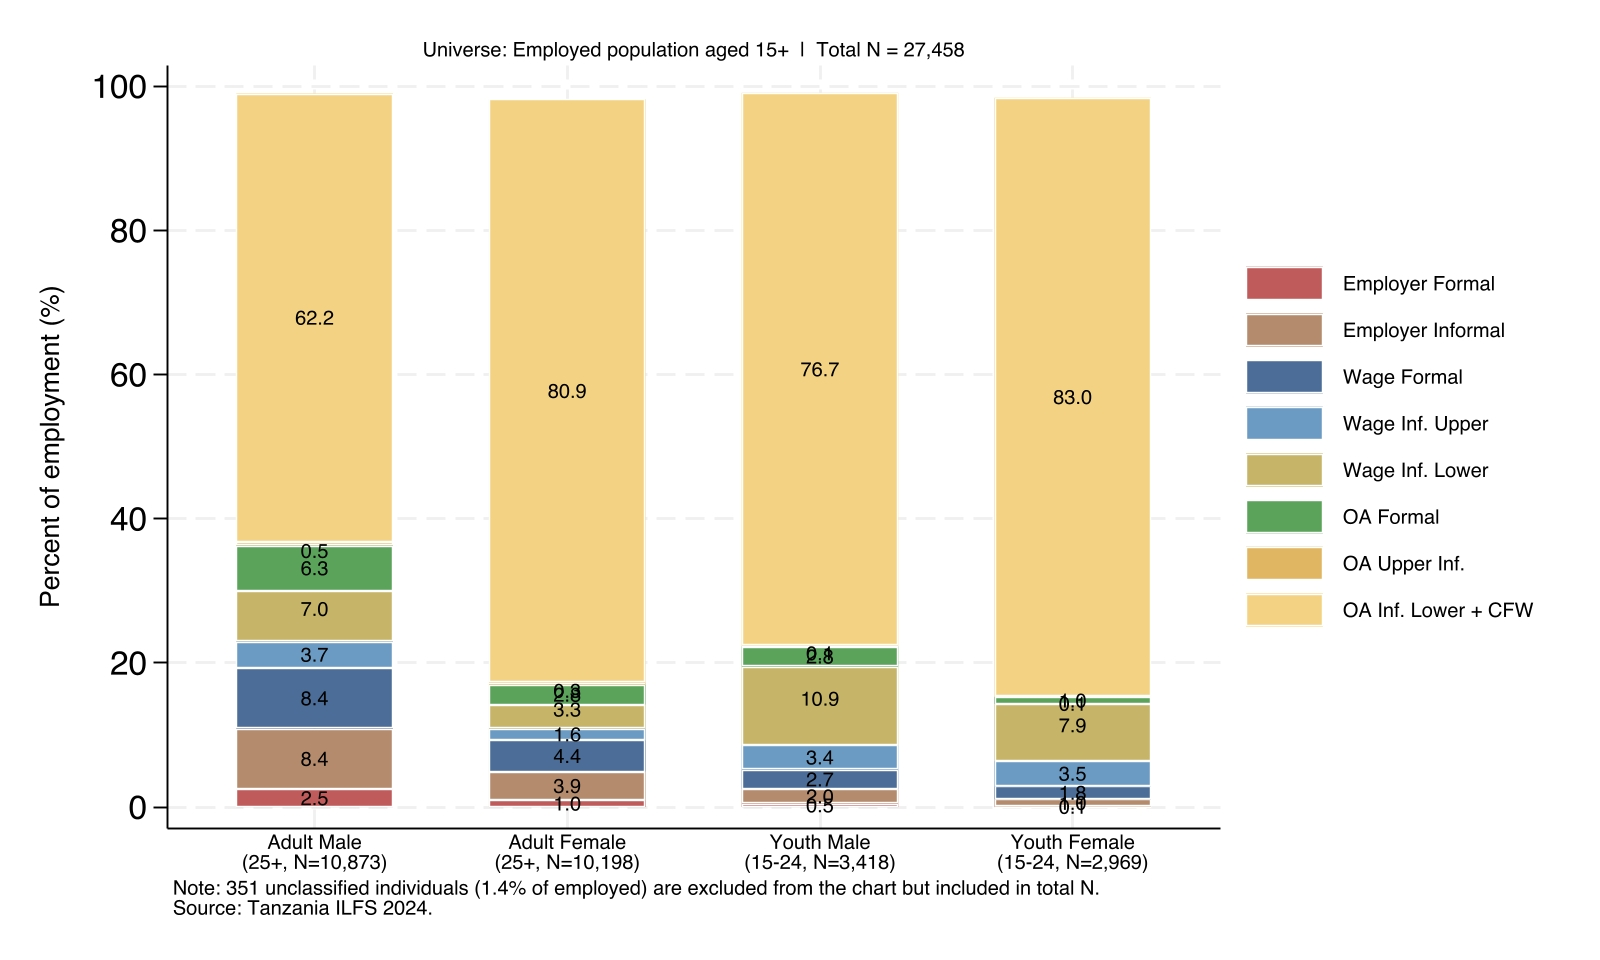
\includegraphics[width=0.85\textwidth]{figures/fig13_youth_vs_all_by_gender.jpg}
  \caption{Youth versus all workers, stacked bars by gender.}
  \label{fig:youth_all}
\end{figure}

Youth (15--24) are more concentrated in OA lower informal plus CFW than adults of the same gender. Among young men the share is 76.7\% against 62.2\% for adults; among young women it is 83.0\% against 80.9\% (Figures~\ref{fig:youth} and~\ref{fig:youth_all}, Table~\ref{tab:youth}). The wage formal share is 2.7\% for young men (vs 6.9\% overall) and 1.8\% for young women (vs 3.8\%). Wage informal lower jobs absorb a slightly larger fraction of young people than of adults in both genders, suggesting that early careers are concentrated either in unpaid family work or in the lower tier of paid work.

\begin{table}[H]
\centering
\caption{Work status: all workers vs youth (15--24), by gender.}
\label{tab:youth}
\begin{tabular}{lrrrr}
\toprule
Work Status & All Male & Youth Male & All Female & Youth Female \\
\midrule
Wage Formal            &  6.9\% &  2.7\% &  3.8\% &  1.8\% \\
Wage Informal Upper    &  3.6\% &  3.4\% &  2.0\% &  3.5\% \\
Wage Informal Lower    &  8.1\% & 10.9\% &  4.4\% &  7.9\% \\
OA Formal              &  5.4\% &  2.8\% &  2.4\% &  1.0\% \\
OA Informal Lower + CFW& 66.0\% & 76.7\% & 81.4\% & 83.0\% \\
\bottomrule
\end{tabular}

\smallskip
\footnotesize\textit{Note:} Youth = aged 15--24. $N$: youth male = 3,418; youth female = 2,969.
\end{table}


% ══════════════════════════════════════════════════════════
\section{Out-of-Labour-Force: Reasons for Not Searching}
\label{sec:olf}
% ══════════════════════════════════════════════════════════

\begin{figure}[H]
  \centering
  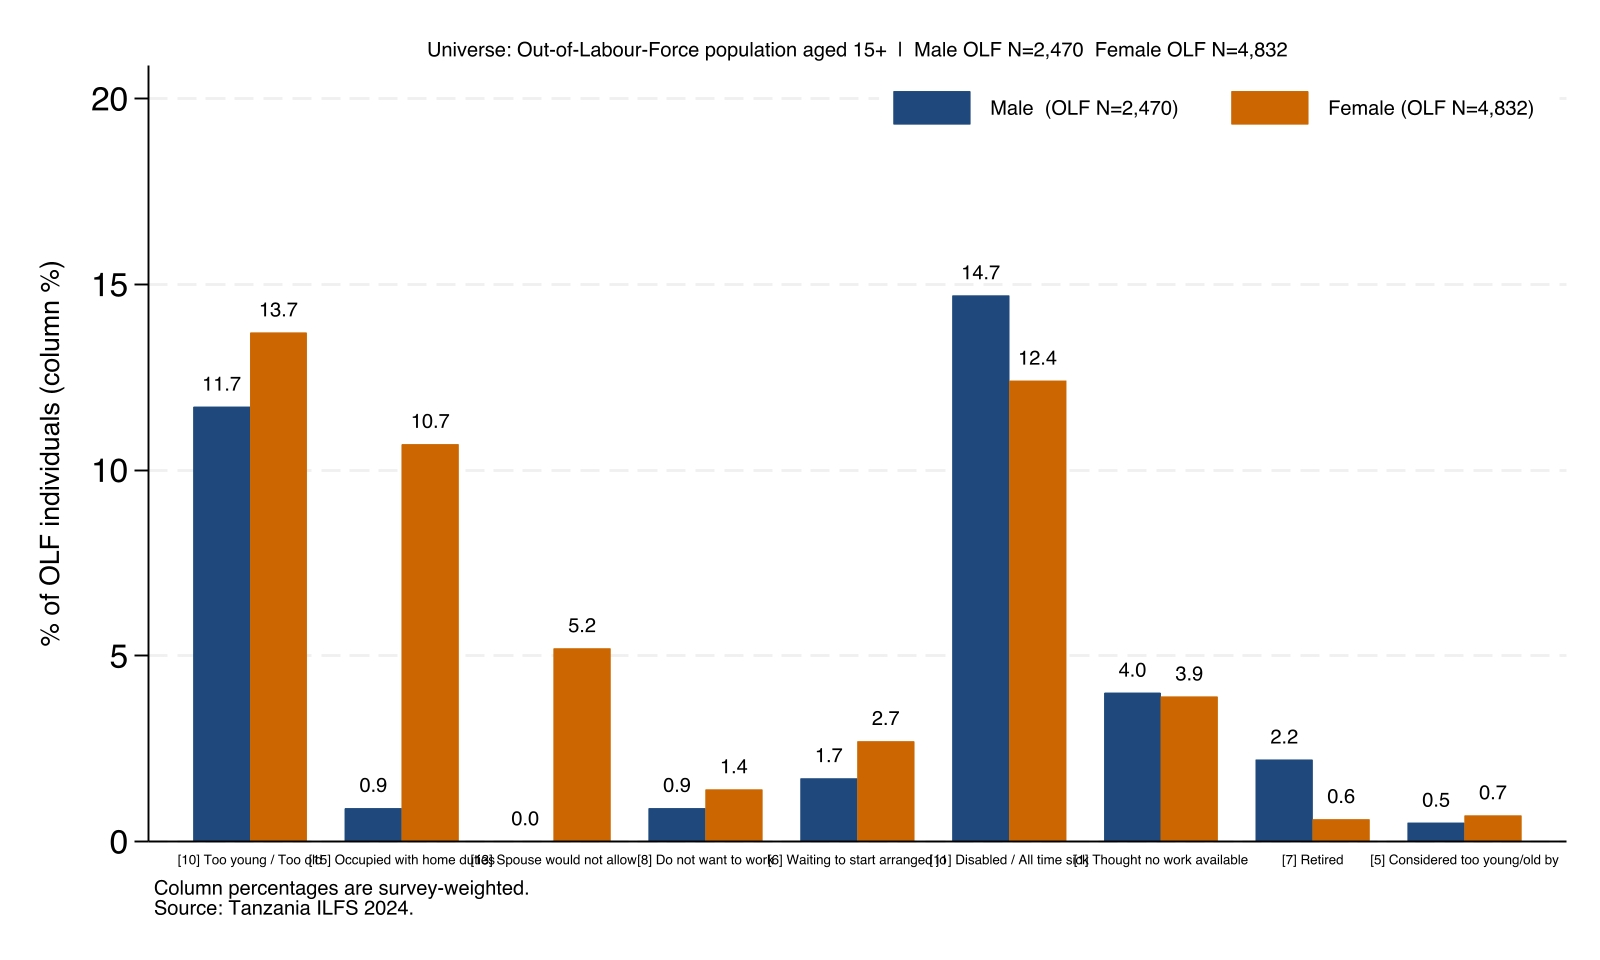
\includegraphics[width=0.85\textwidth]{figures/fig09_reasons_not_searching.jpg}
  \caption{Reasons for not searching for work by gender, out-of-labour-force population.}
  \label{fig:reasons}
\end{figure}

The reasons given by out-of-labour-force respondents for not searching diverge sharply between genders (Figure~\ref{fig:reasons}). Child or family care is reported by 10.7\% of OLF women against 0.9\% of OLF men, and 5.2\% of women cite pregnancy or maternity (against zero for men). Men are more likely to report seasonal factors (14.7\% vs 12.4\%) and retirement or old age (2.2\% vs 0.6\%). Together these patterns account for most of the gender gap in OLF status documented in Section~\ref{sec:lfs}.

\footnotesize\textit{Note:} Column percentages over all OLF individuals. Universe: OLF aged 15+, $N = 7{,}302$ (male = 2,470; female = 4,832).
\normalsize


% ══════════════════════════════════════════════════════════
\section{Public, Private and Online Work}
\label{sec:online}
% ══════════════════════════════════════════════════════════

\subsection{Public versus private sector}

Public-sector employment is concentrated almost entirely in wage formal jobs: 48.5\% of wage formal workers are employed by central or local government or by parastatals, against 11.7\% in wage informal upper, 3.5\% in wage informal lower, and effectively zero in employer or own-account categories (Figure~\ref{fig:public_private}, Table~\ref{tab:public_private}). The corollary is that policy levers operating through public employment reach only a small share of the labour market.

\begin{figure}[H]
  \centering
  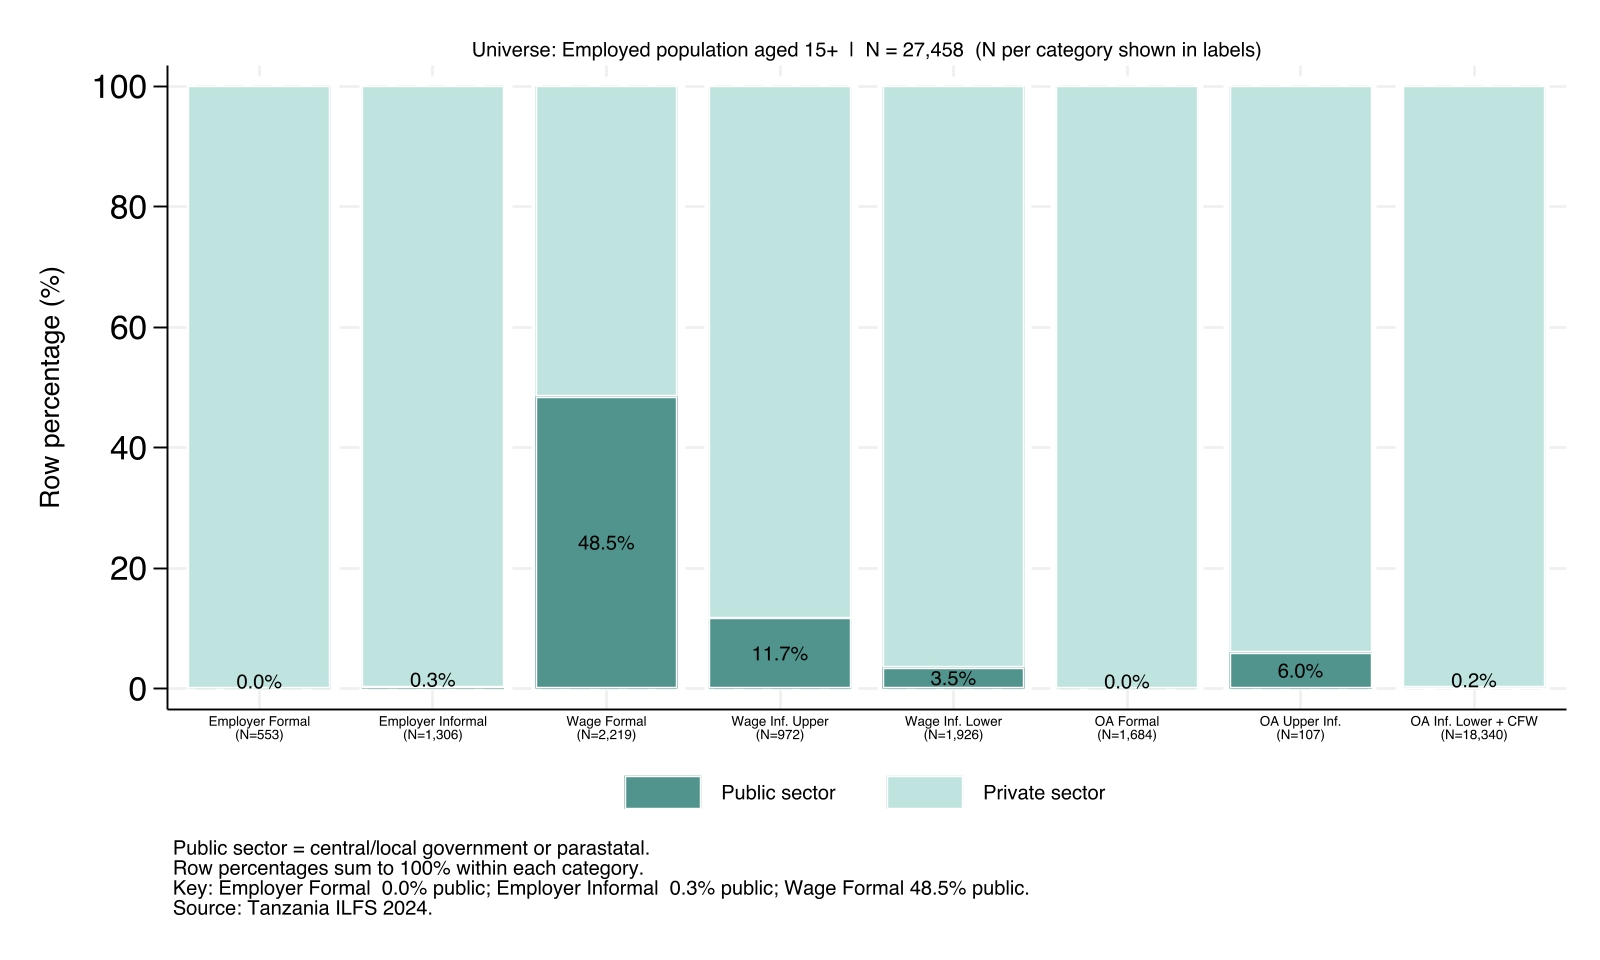
\includegraphics[width=0.85\textwidth]{figures/fig10_public_private_sector.jpg}
  \caption{Public versus private sector by work status.}
  \label{fig:public_private}
\end{figure}

\begin{table}[H]
\centering
\caption{Public versus private sector by work status.}
\label{tab:public_private}
\begin{tabular}{lrrr}
\toprule
Work Status & $N$ & Public \% & Private \% \\
\midrule
Employer Formal        &   553  &  0.0\% & 100.0\% \\
Employer Inf.\ Upper   & 1,306  &  0.3\% &  99.7\% \\
Wage Formal            & 2,219  & 48.5\% &  51.5\% \\
Wage Informal Upper    &   972  & 11.7\% &  88.3\% \\
Wage Informal Lower    & 1,926  &  3.5\% &  96.5\% \\
OA Formal              & 1,684  &  0.0\% & 100.0\% \\
OA Upper Informal      &   107  &  6.0\% &  94.0\% \\
OA Informal Lower + CFW&18,340  &  0.2\% &  99.8\% \\
\bottomrule
\end{tabular}

\smallskip
\footnotesize\textit{Note:} Public sector = central/local government or parastatal (Q37 codes 1--3).
\end{table}

\subsection{Online work (Q24)}

Online participation is rare overall. Within OA lower informal and CFW the share is roughly 1.3--1.4\% for both genders, and in wage informal lower it remains under 5\% (Figure~\ref{fig:online}, Table~\ref{tab:online}). Higher-tier categories show non-trivial uptake: 23.5\% of male employer formal workers and 29.9\% of female employer formal workers report online work, and women in wage informal upper and OA formal also exceed men. The OA upper informal cell shows a 18.5-point male-female gap (18.6\% vs 0.1\%) that stems from very small samples and should be read alongside Section~\ref{sec:educ_formal}.

\begin{figure}[H]
  \centering
  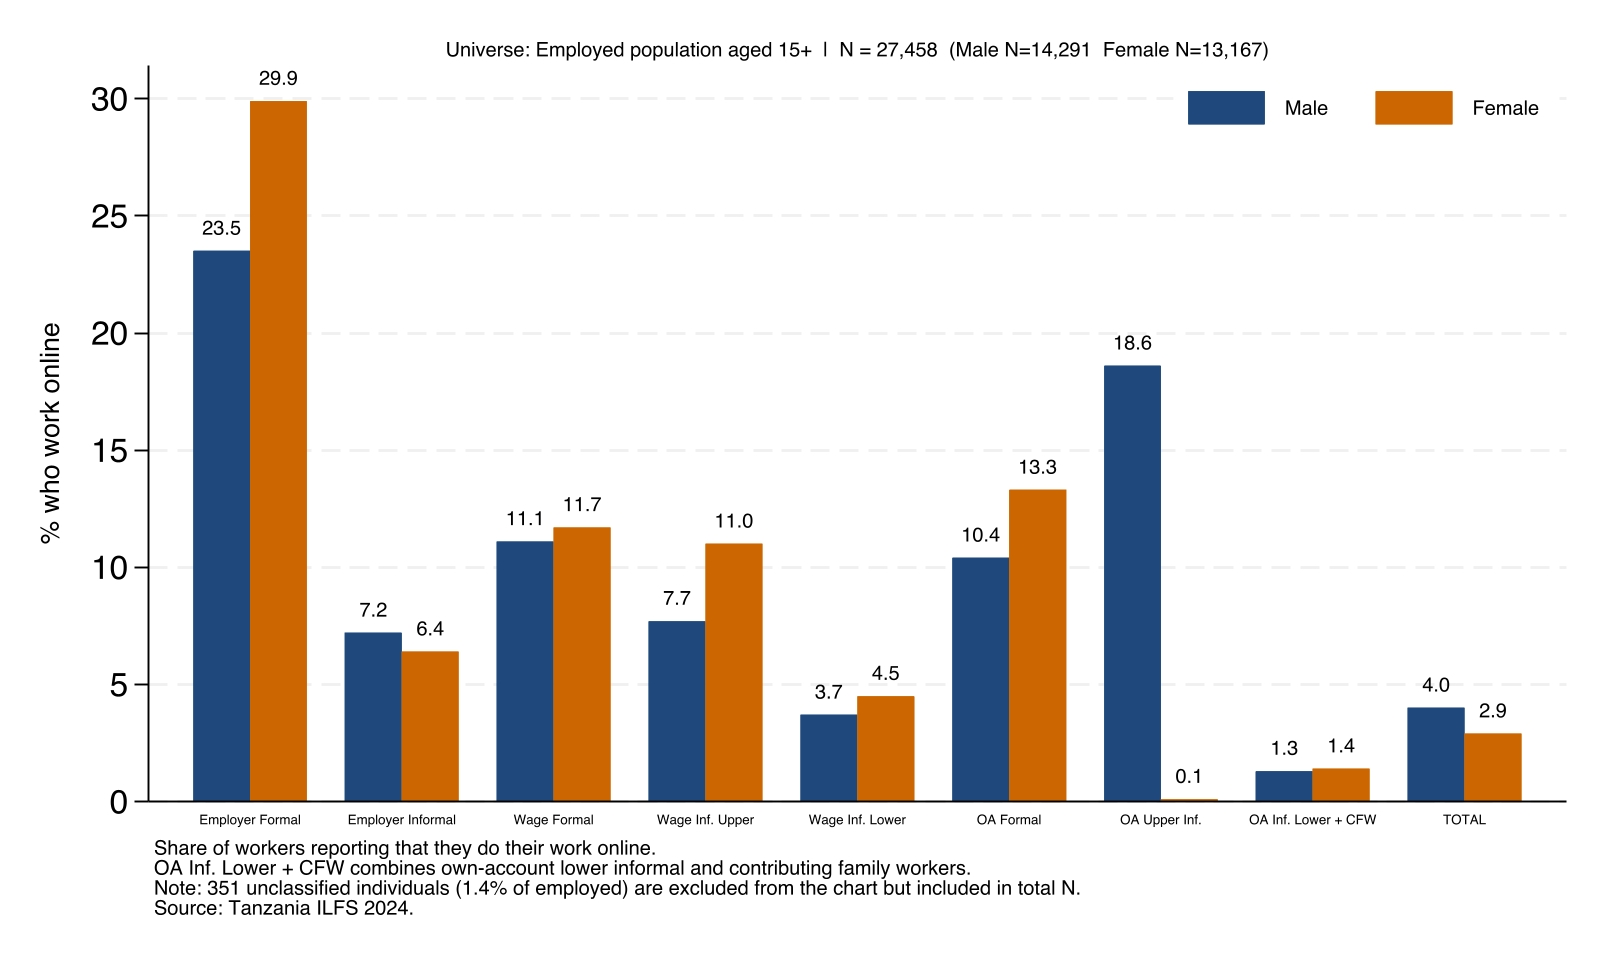
\includegraphics[width=0.85\textwidth]{figures/fig14_q24_online_work.jpg}
  \caption{Share of employed workers reporting online work (Q24), by work status and gender.}
  \label{fig:online}
\end{figure}

\begin{figure}[H]
  \centering
  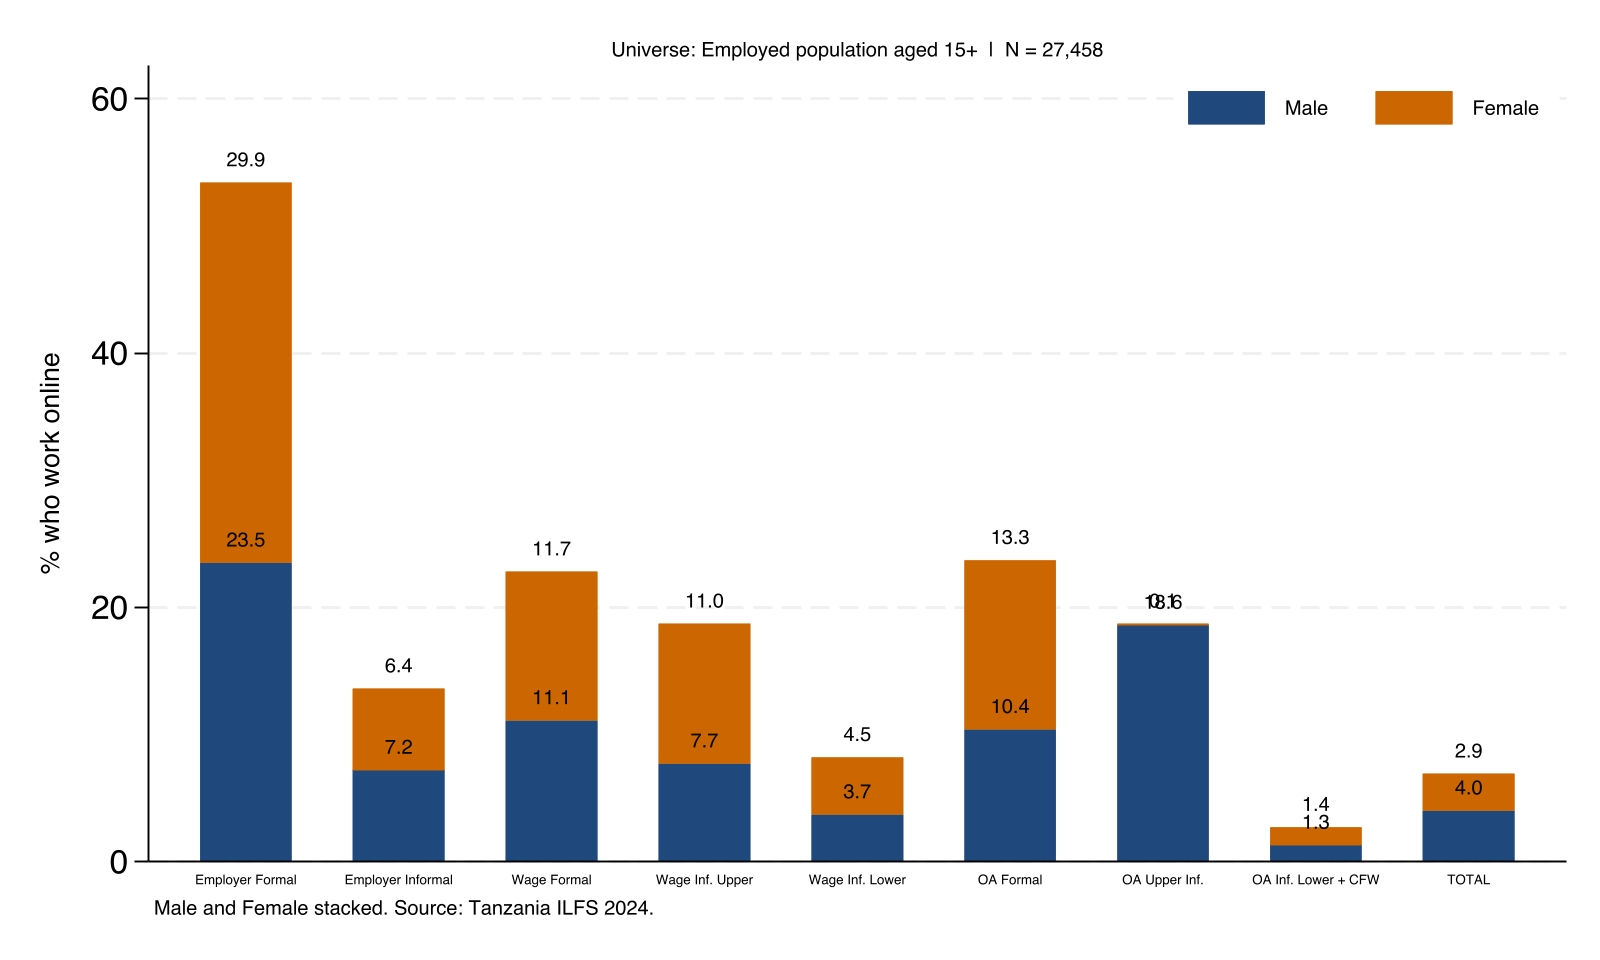
\includegraphics[width=0.85\textwidth]{figures/fig14b_q24_online_stacked.jpg}
  \caption{Online work (Q24) by work status, male/female stacked contribution.}
  \label{fig:online_stacked}
\end{figure}

\begin{figure}[H]
  \centering
  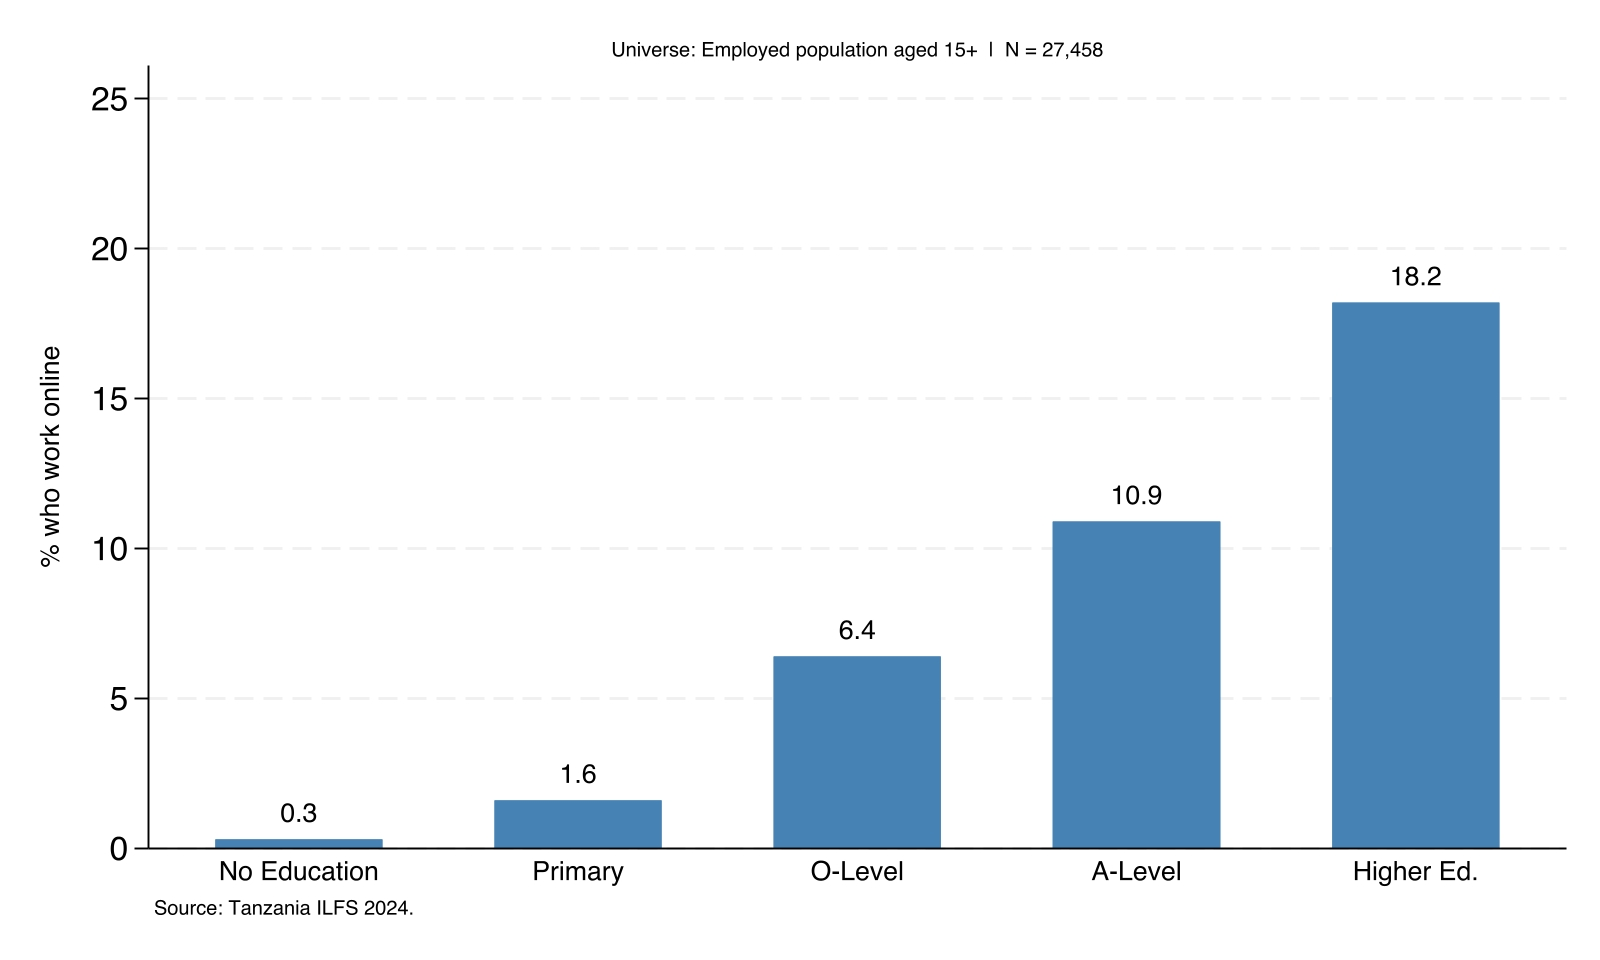
\includegraphics[width=0.85\textwidth]{figures/fig14c_q24_online_education.jpg}
  \caption{Online work (Q24) by education level (employed, aged 15+).}
  \label{fig:online_educ}
\end{figure}

The breakdown by education (Figure~\ref{fig:online_educ}) shows a steep gradient with schooling, which together with the work-status pattern confirms that digital participation is heavily filtered by formal-sector access and human capital. Geographical variation is taken up in Section~\ref{sec:location}.

\begin{table}[H]
\centering
\caption{Online work (Q24) by work status and gender.}
\label{tab:online}
\begin{tabular}{lrrr}
\toprule
Work Status & Male Online \% & Female Online \% & Gap (F$-$M, pp) \\
\midrule
Employer Formal        & 23.5\% & 29.9\% & +6.4 \\
Employer Inf.\ Upper   &  7.2\% &  6.4\% & $-$0.8 \\
Wage Formal            & 11.1\% & 11.7\% & +0.6 \\
Wage Informal Upper    &  7.7\% & 11.0\% & +3.3 \\
Wage Informal Lower    &  3.7\% &  4.5\% & +0.8 \\
OA Formal              & 10.4\% & 13.3\% & +2.9 \\
OA Upper Informal      & 18.6\% &  0.1\% & $-$18.5 \\
OA Informal Lower + CFW&  1.3\% &  1.4\% & +0.1 \\
\bottomrule
\end{tabular}

\smallskip
\footnotesize\textit{Note:} Q24: ``Do you do your work/activity online?'' Share answering yes. OA upper informal female cell has small sample.
\end{table}


% ══════════════════════════════════════════════════════════
\section{Sectoral Patterns}
\label{sec:sectors}
% ══════════════════════════════════════════════════════════

\subsection{Sector by work status, main and secondary jobs}

Sectoral segmentation in job quality is pronounced (Figure~\ref{fig:sector_main}). Lower-tier informality (wage informal lower, OA lower informal and CFW combined) accounts for 93.6\% of agricultural employment and 71.9\% of manufacturing employment. Construction stands out for its large upper-informal segment (34.9\%), while public administration (73.7\% wage formal) and education (78.2\%) are dominated by formal wage work. Wholesale and retail and accommodation and food services are intermediate, with wage formal shares between 10\% and 18\%.

\begin{figure}[H]
  \centering
  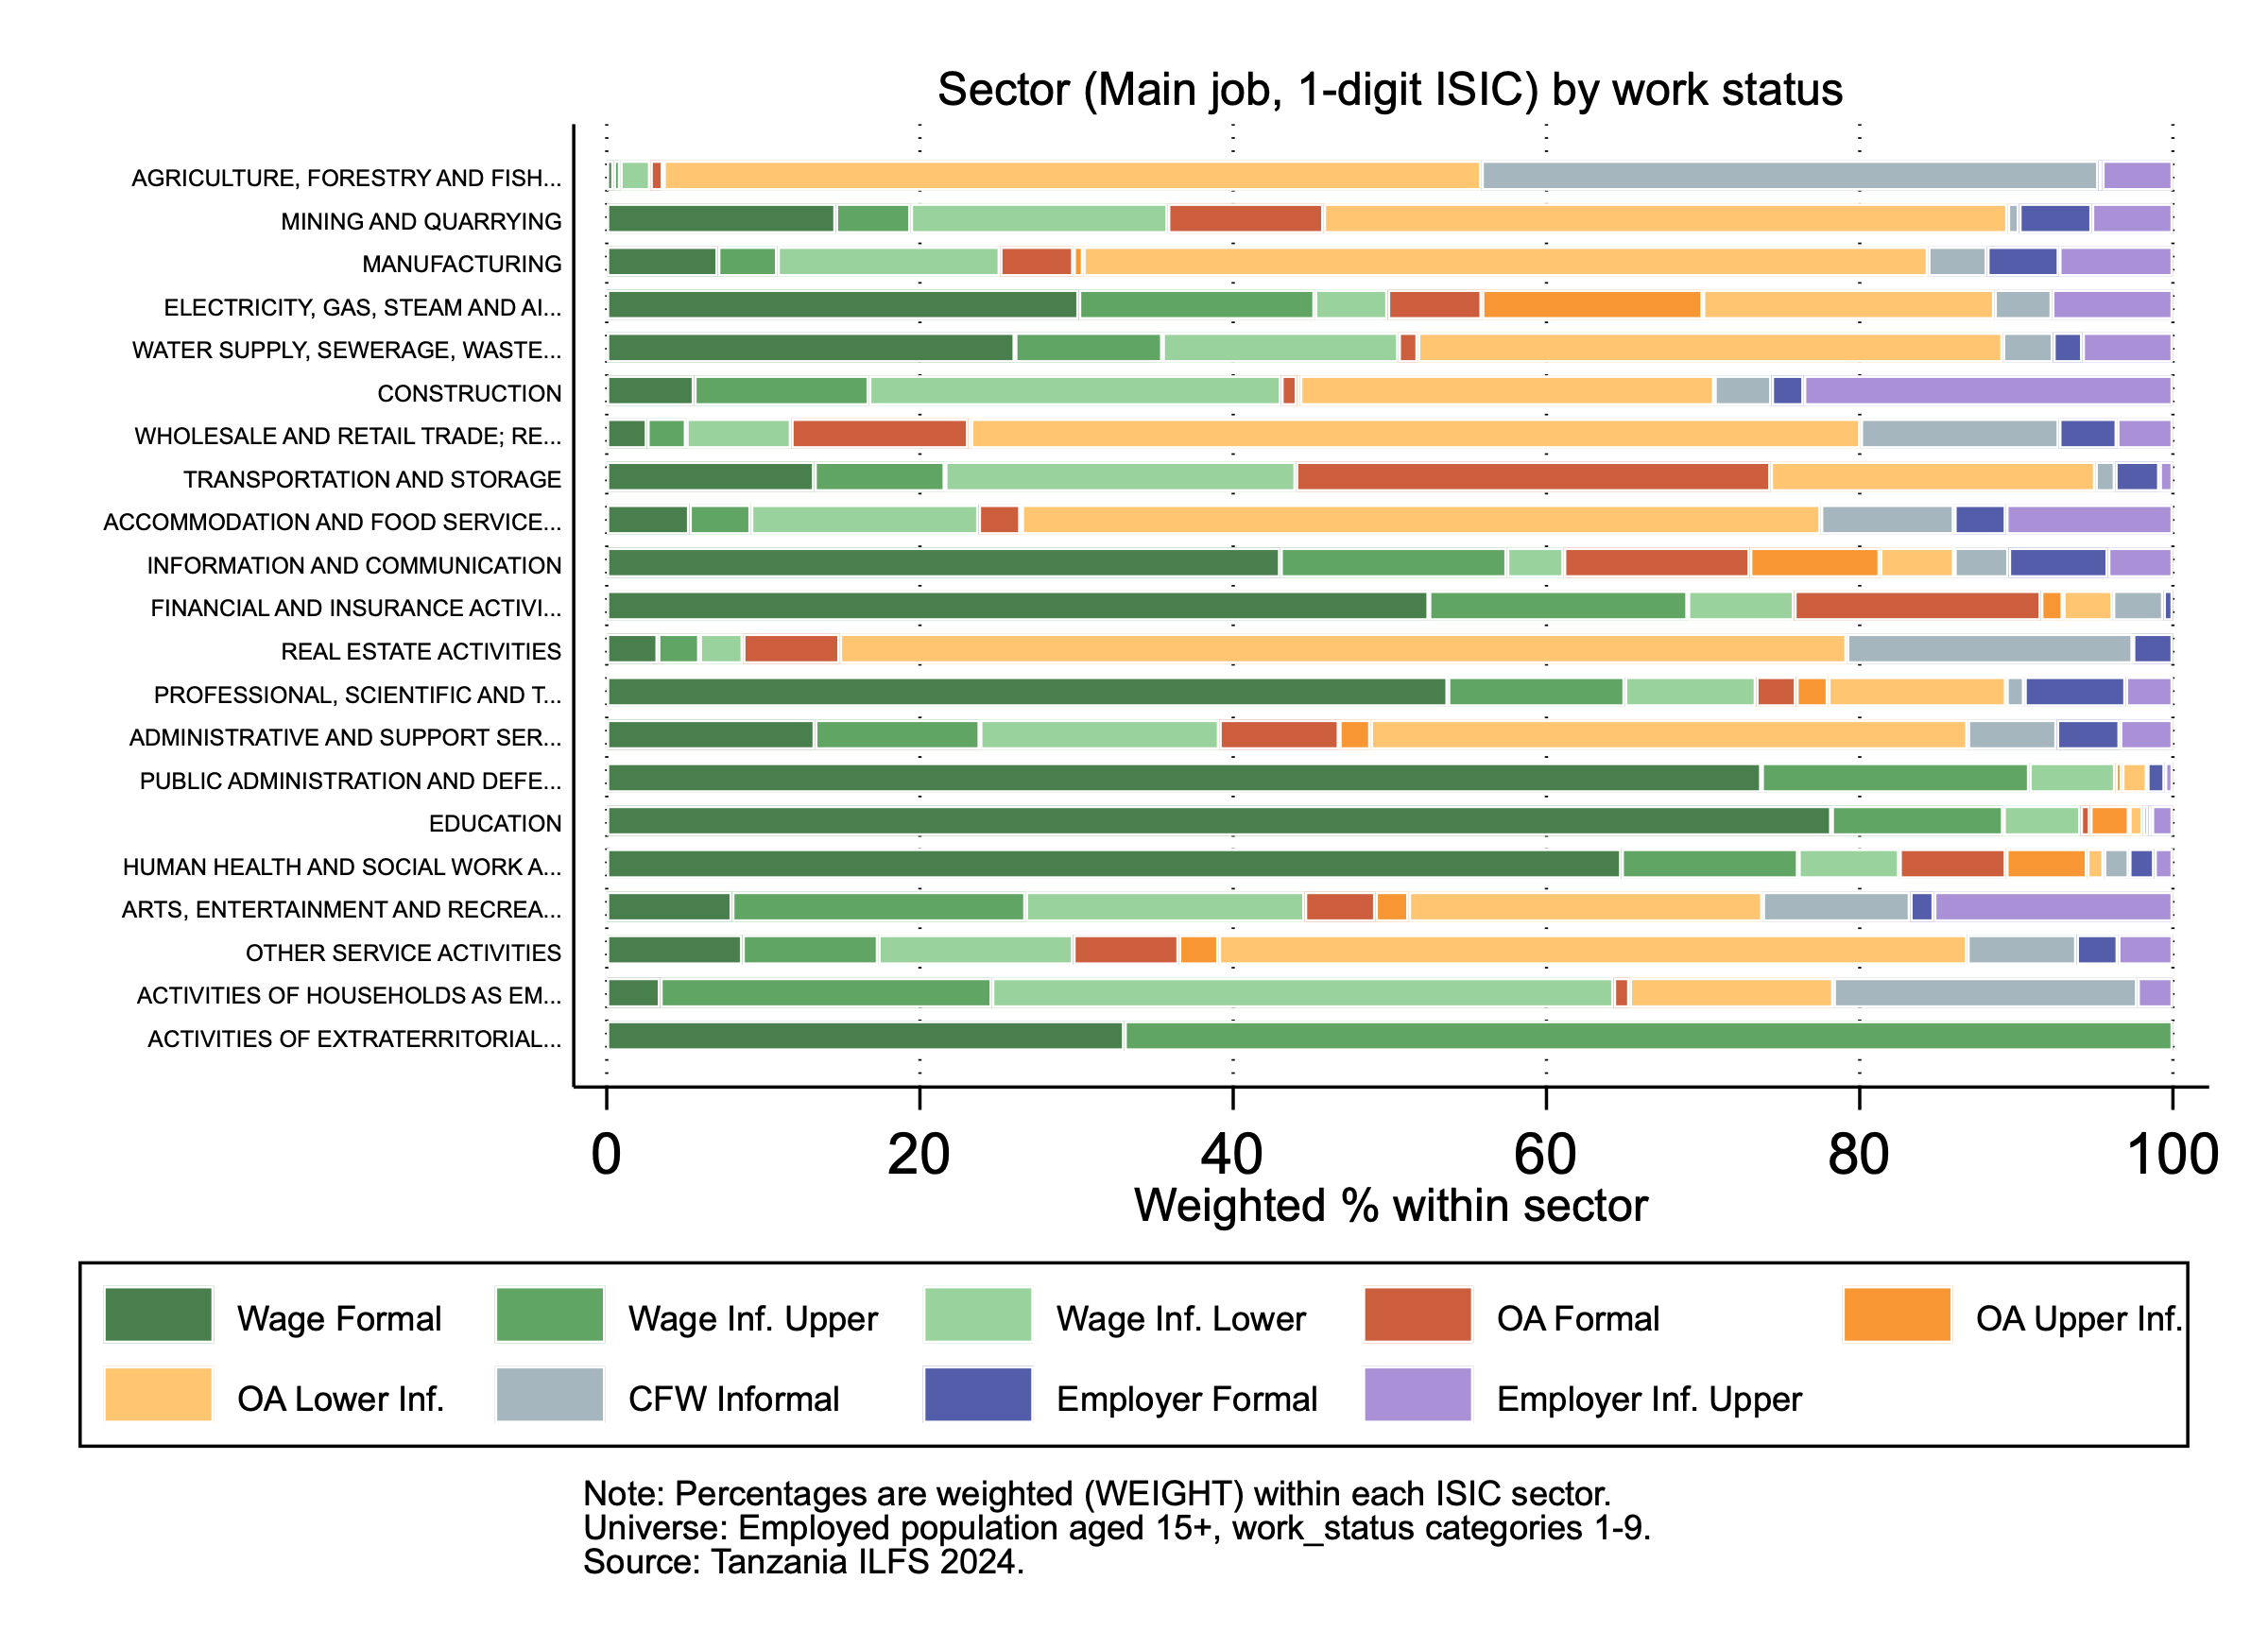
\includegraphics[width=\textwidth]{figures/fig16_sector_workstatus_main.jpg}
  \caption{Sector by work status composition (main job, ISIC 1-digit).}
  \label{fig:sector_main}
\end{figure}

Secondary jobs (Figure~\ref{fig:sector_secondary}) are systematically more informal than main jobs. OA lower informal becomes the largest category in most sectors (52.3\% in agriculture, 64.0\% in manufacturing), with CFW adding further weight at the bottom of the ladder.

\begin{figure}[H]
  \centering
  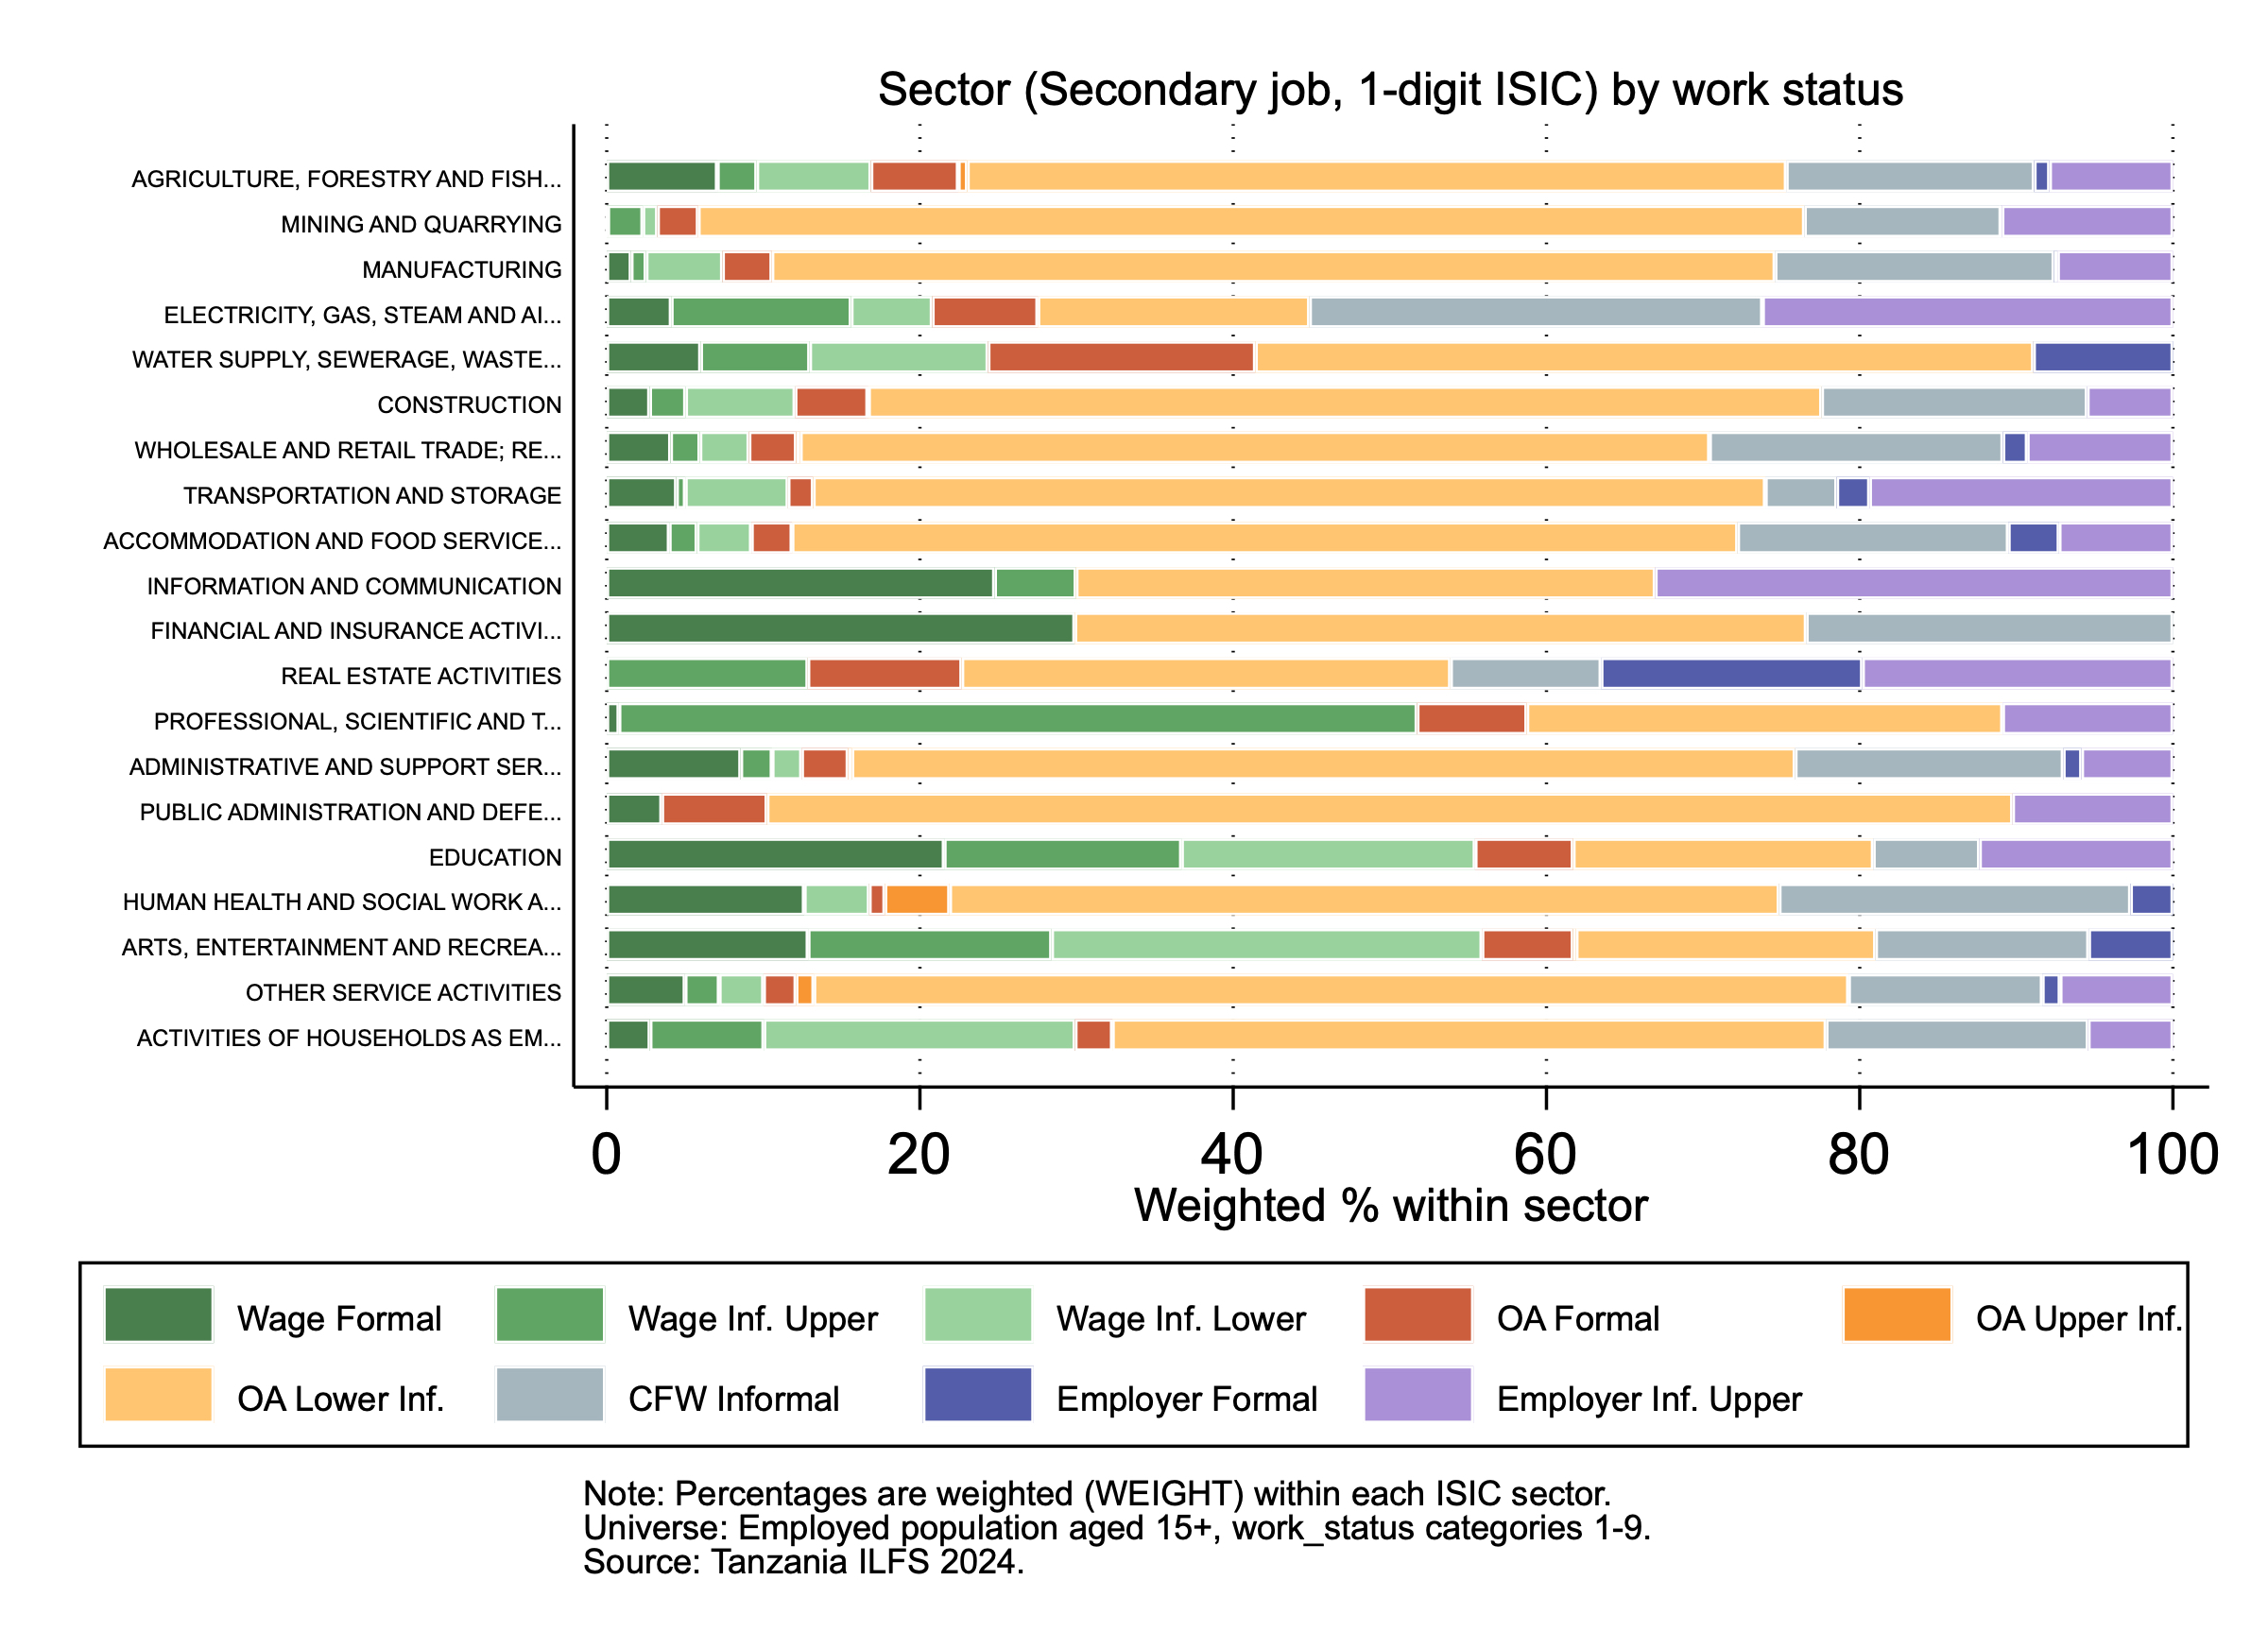
\includegraphics[width=\textwidth]{figures/fig17_sector_workstatus_secondary.jpg}
  \caption{Sector by work status composition (secondary job, ISIC 1-digit).}
  \label{fig:sector_secondary}
\end{figure}

\subsection{Manufacturing sub-sectors}

Manufacturing employment is concentrated in three sub-sectors: textiles (24.9\%), wood products (13.1\%) and food products (9.9\%) (Figure~\ref{fig:manuf_comp}). Within these, lower-tier informality dominates: wearing apparel reaches 90.9\% and textiles 86.6\% (Figure~\ref{fig:manuf_informality}). The two sub-sectors with the highest formal shares---chemicals (31.9\%) and motor vehicles (29.1\%)---together represent a small share of total manufacturing employment.

\begin{figure}[H]
  \centering
  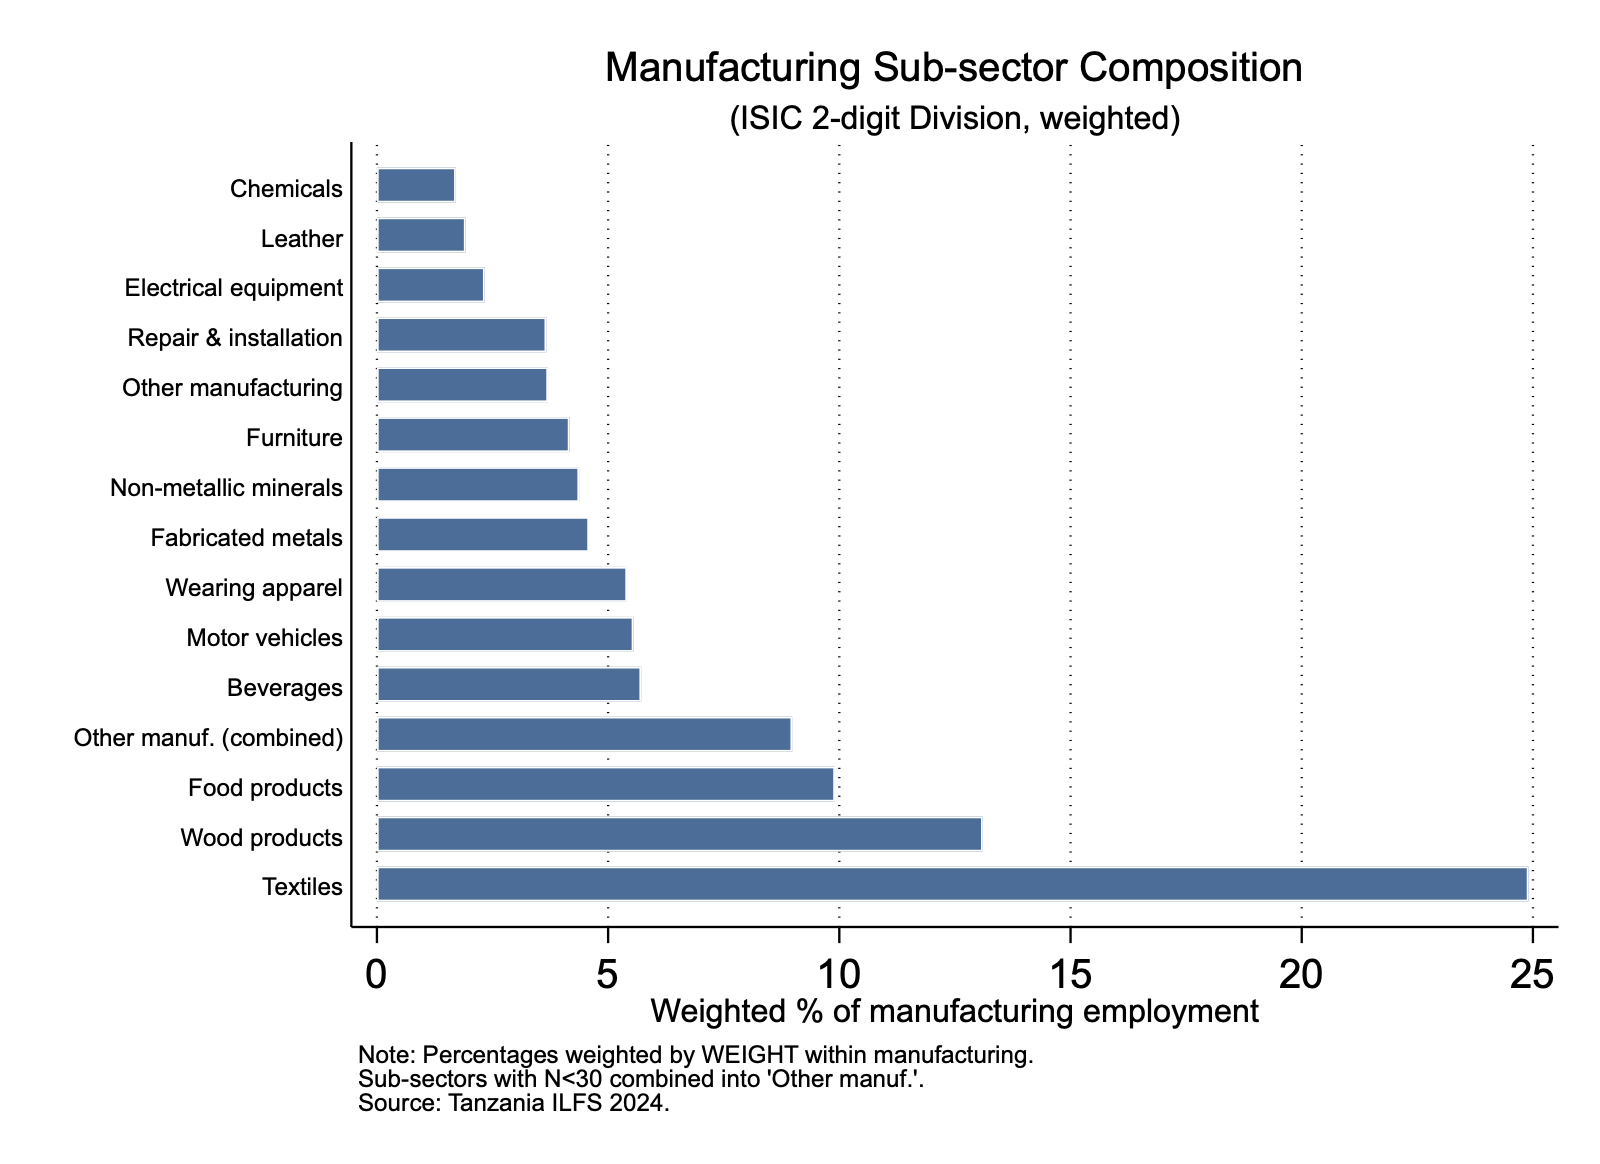
\includegraphics[width=0.9\textwidth]{figures/fig18_manuf_subsector_composition.jpg}
  \caption{Manufacturing sub-sector composition.}
  \label{fig:manuf_comp}
\end{figure}

\begin{figure}[H]
  \centering
  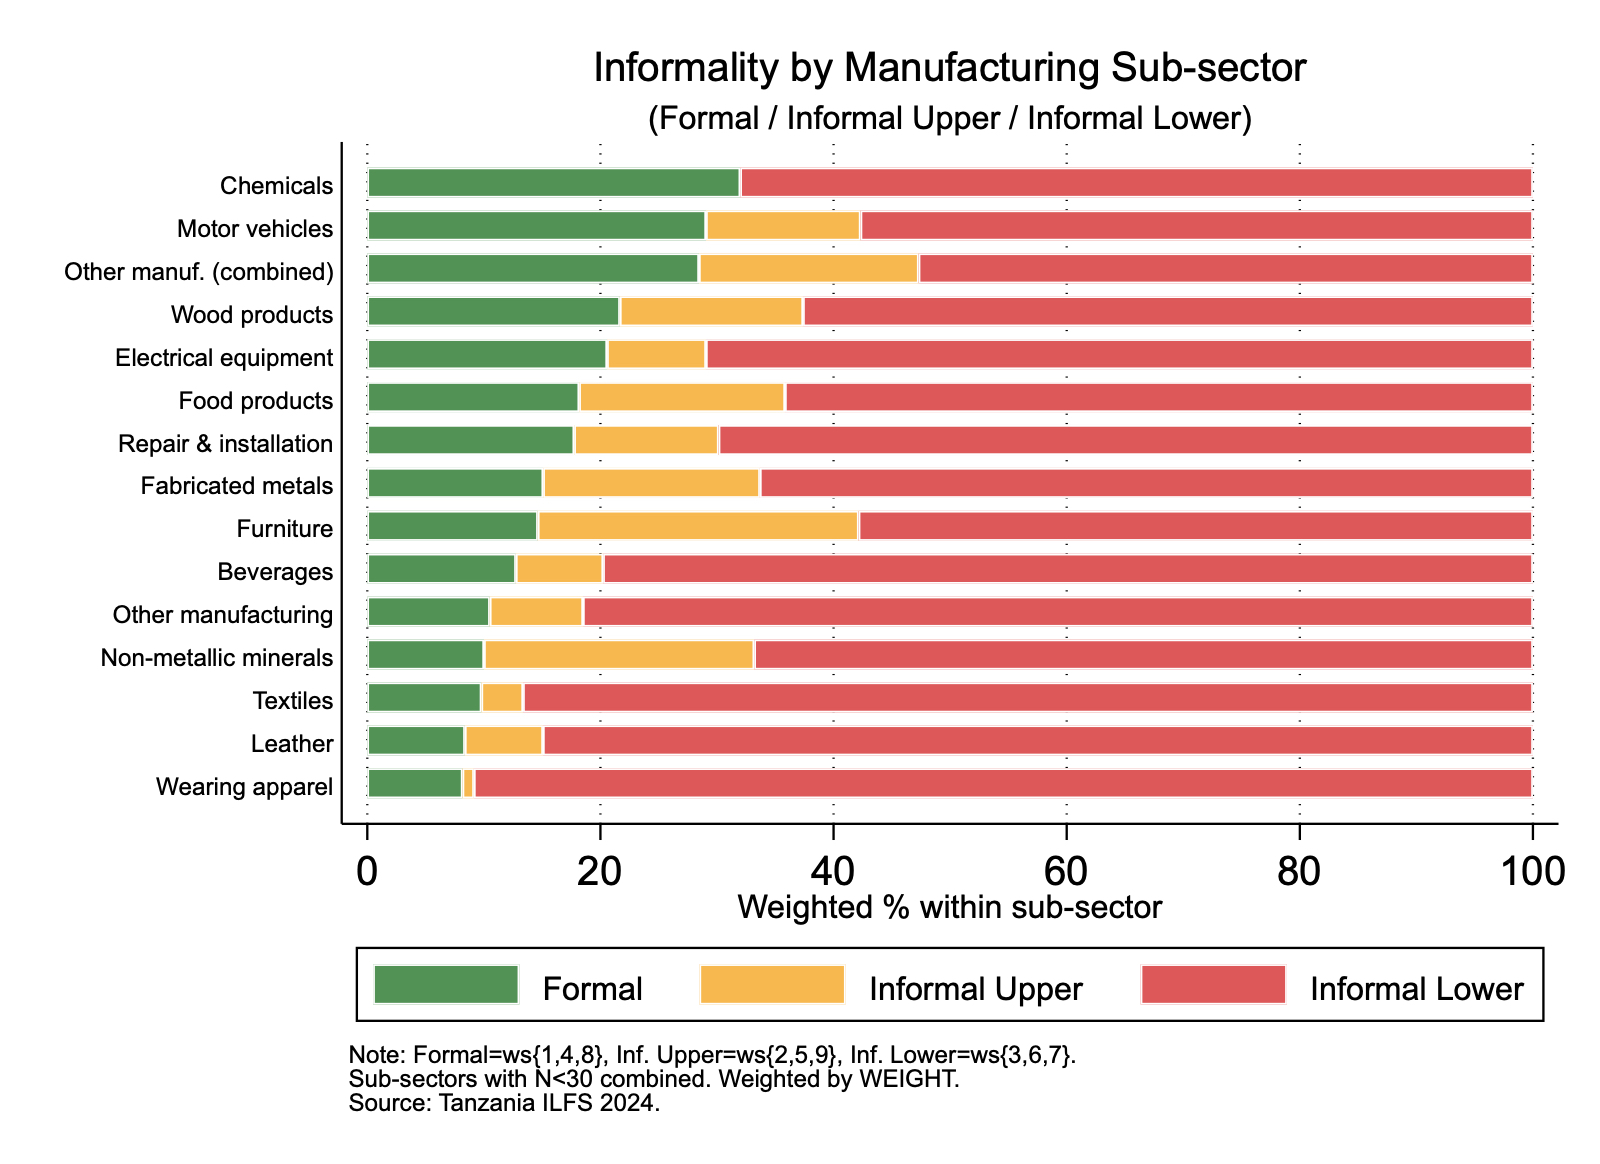
\includegraphics[width=0.9\textwidth]{figures/fig19_manuf_informality_by_subsector.jpg}
  \caption{Informality structure by manufacturing sub-sector.}
  \label{fig:manuf_informality}
\end{figure}

Gender segregation across manufacturing sub-sectors is severe (Figure~\ref{fig:manuf_gender}). Wearing apparel (85.7\% female) and textiles (84.0\% female) are largely female; fabricated metals (98.7\% male) and motor vehicles (98.2\% male) are almost entirely male. The cross-sector summary (Figure~\ref{fig:sector_informality_compare}) places these patterns alongside other major sectors: formal shares are 1.5\% in agriculture, 17.6\% in wholesale and retail, and 16.4\% in manufacturing, while lower-tier informality remains above 56\% in all five sectors shown.

\begin{figure}[H]
  \centering
  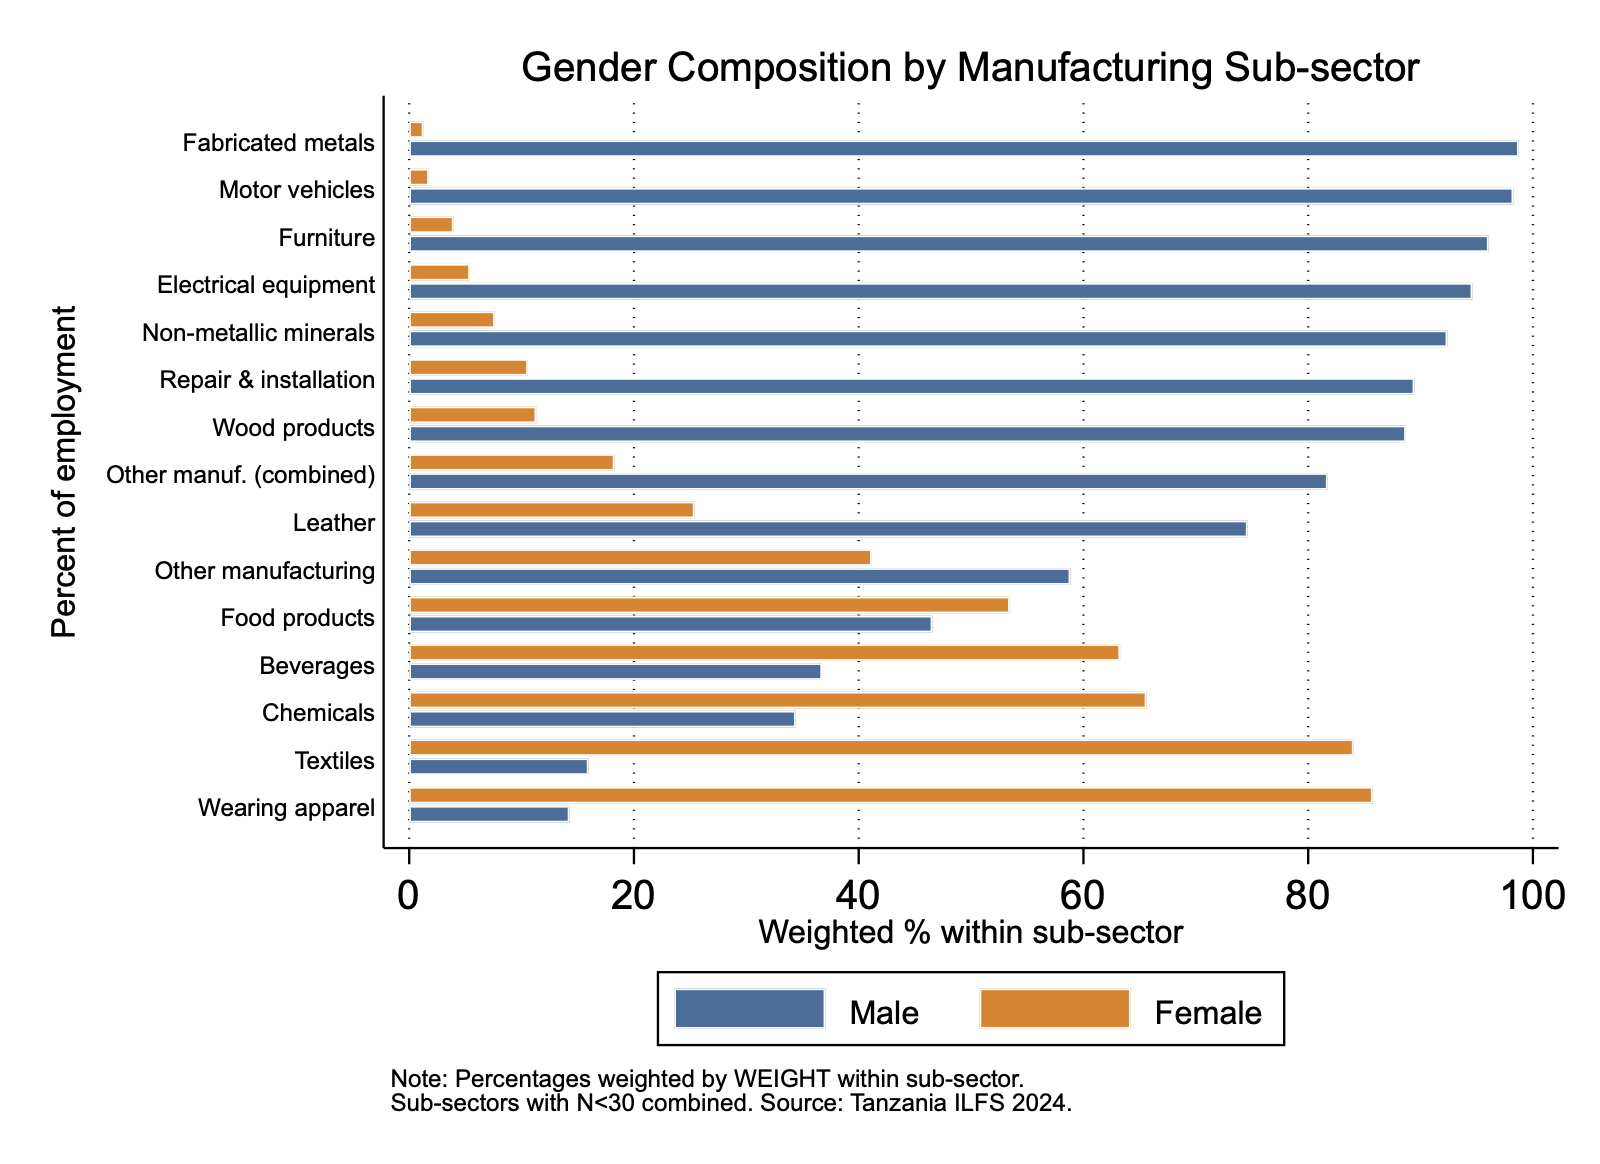
\includegraphics[width=0.9\textwidth]{figures/fig20_manuf_gender_by_subsector.jpg}
  \caption{Gender composition by manufacturing sub-sector.}
  \label{fig:manuf_gender}
\end{figure}

\begin{figure}[H]
  \centering
  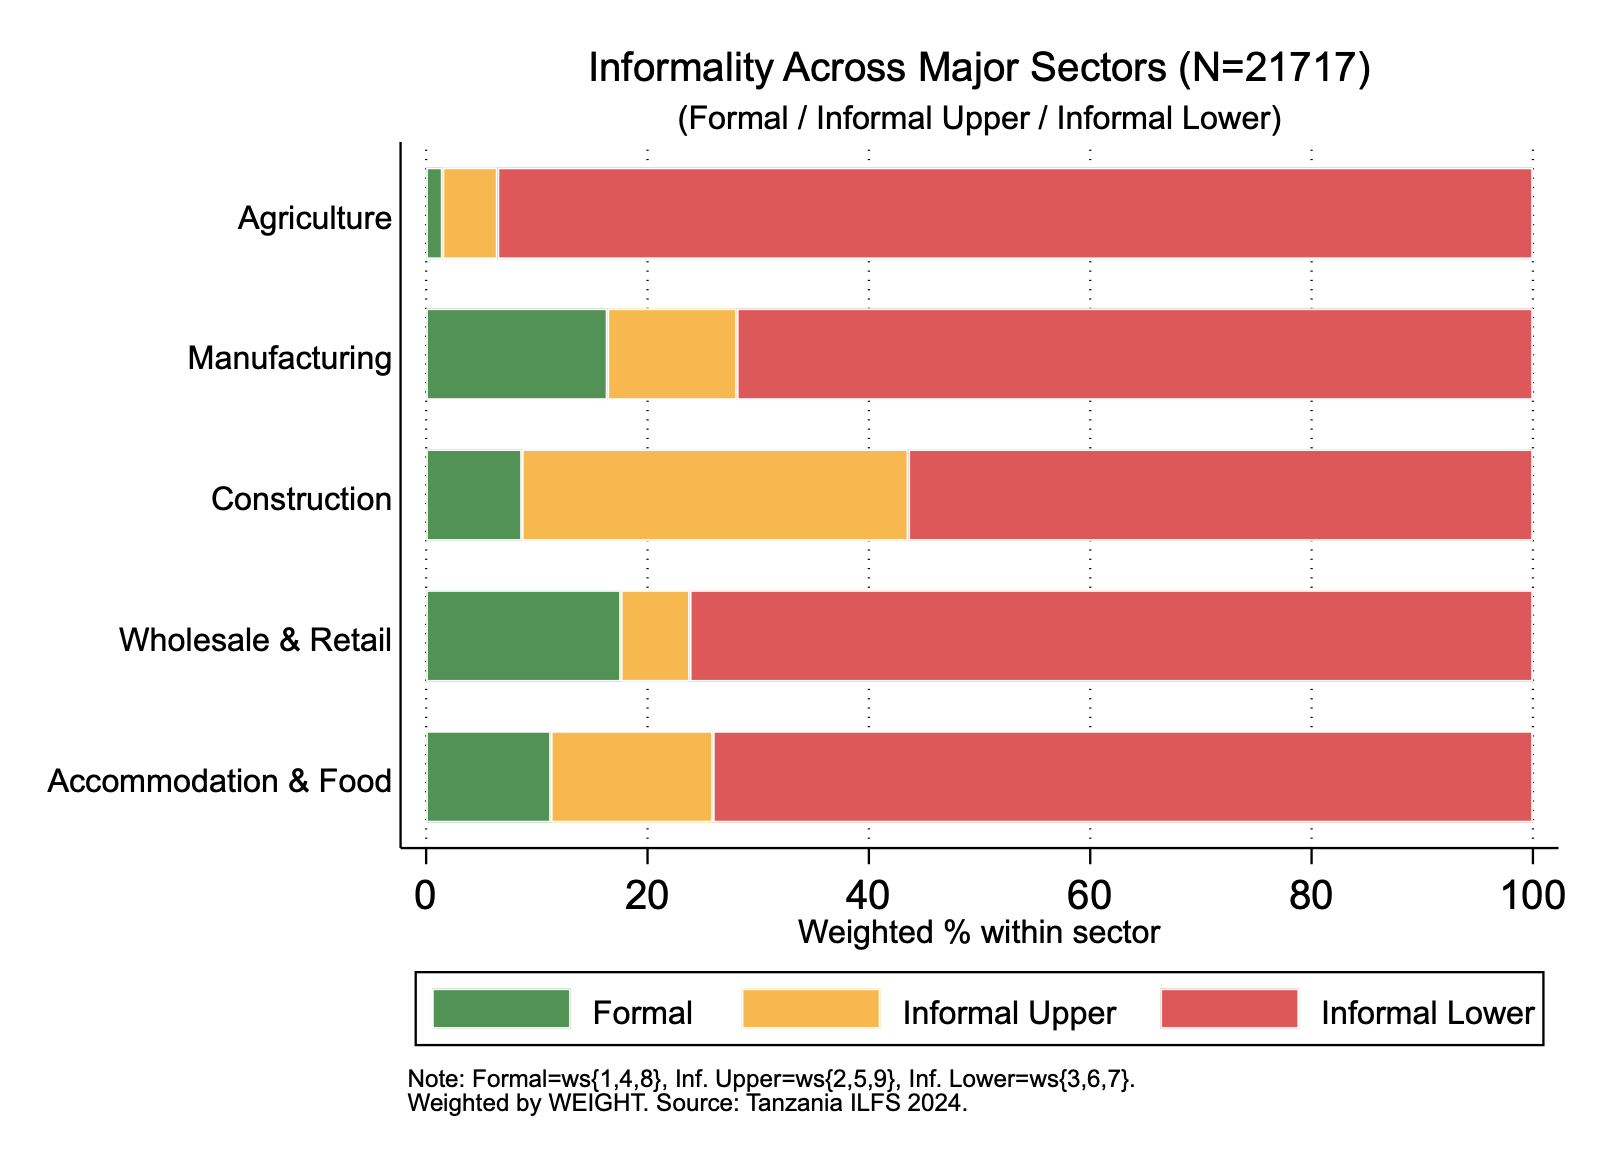
\includegraphics[width=0.85\textwidth]{figures/fig21_sector_informality_compare.jpg}
  \caption{Formal versus upper- and lower-tier informal shares across selected major sectors.}
  \label{fig:sector_informality_compare}
\end{figure}


% ══════════════════════════════════════════════════════════
\section{Informal Enterprise Motives and Credit}
\label{sec:informal_credit}
% ══════════════════════════════════════════════════════════

The Q45B (reasons for starting a business) and Q47A/B (credit access and source) modules apply primarily to non-wage workers. Coverage is near-zero in wage categories by survey design and reaches 99.4\% in OA lower informal and 93.8\% in employer informal upper (Figure~\ref{fig:q45q47_coverage}).

\begin{figure}[H]
  \centering
  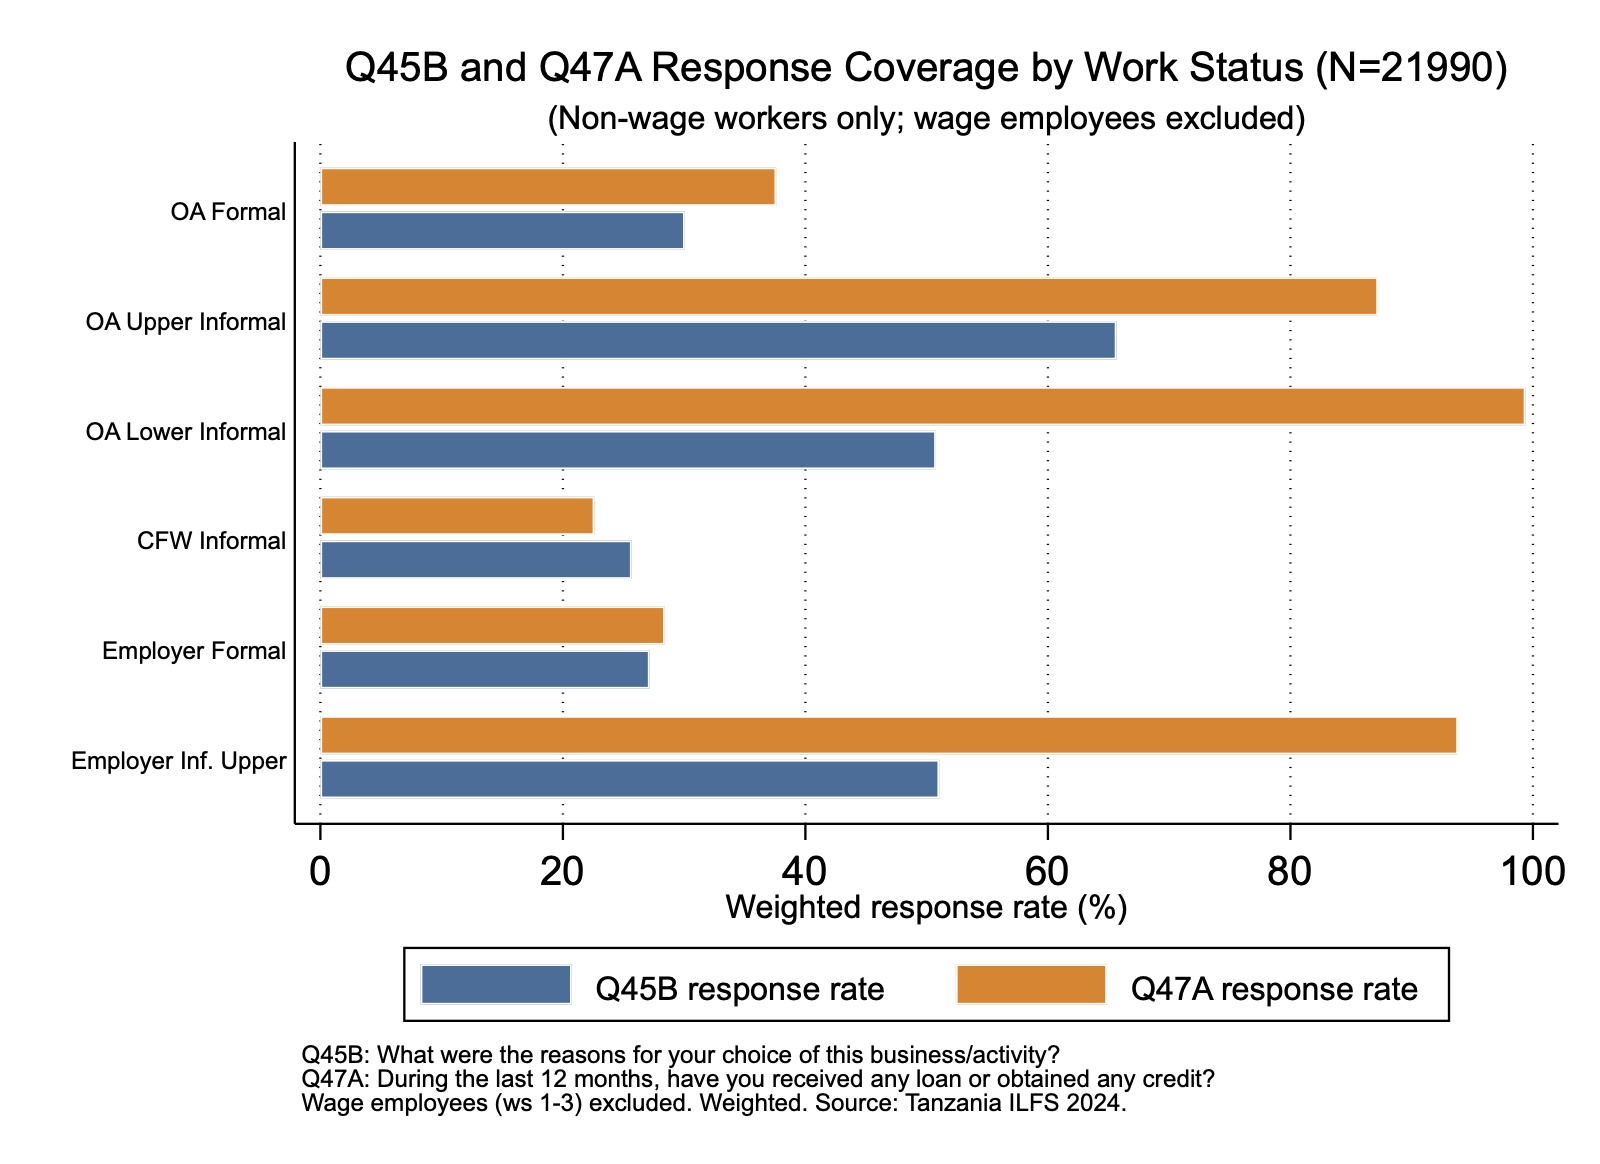
\includegraphics[width=0.9\textwidth]{figures/fig22_q45b_q47a_coverage.jpg}
  \caption{Q45B/Q47A response coverage by work status.}
  \label{fig:q45q47_coverage}
\end{figure}

Across sectors, ``family needs additional income'' and ``low start-up capital'' are the most common motives for entry into the activity. The relative weight of ``good income opportunities'' is higher in construction (37.5\%) than in agriculture (20.2\%), pointing to genuine pull factors only in some segments (Figure~\ref{fig:q45_reasons}).

\begin{figure}[H]
  \centering
  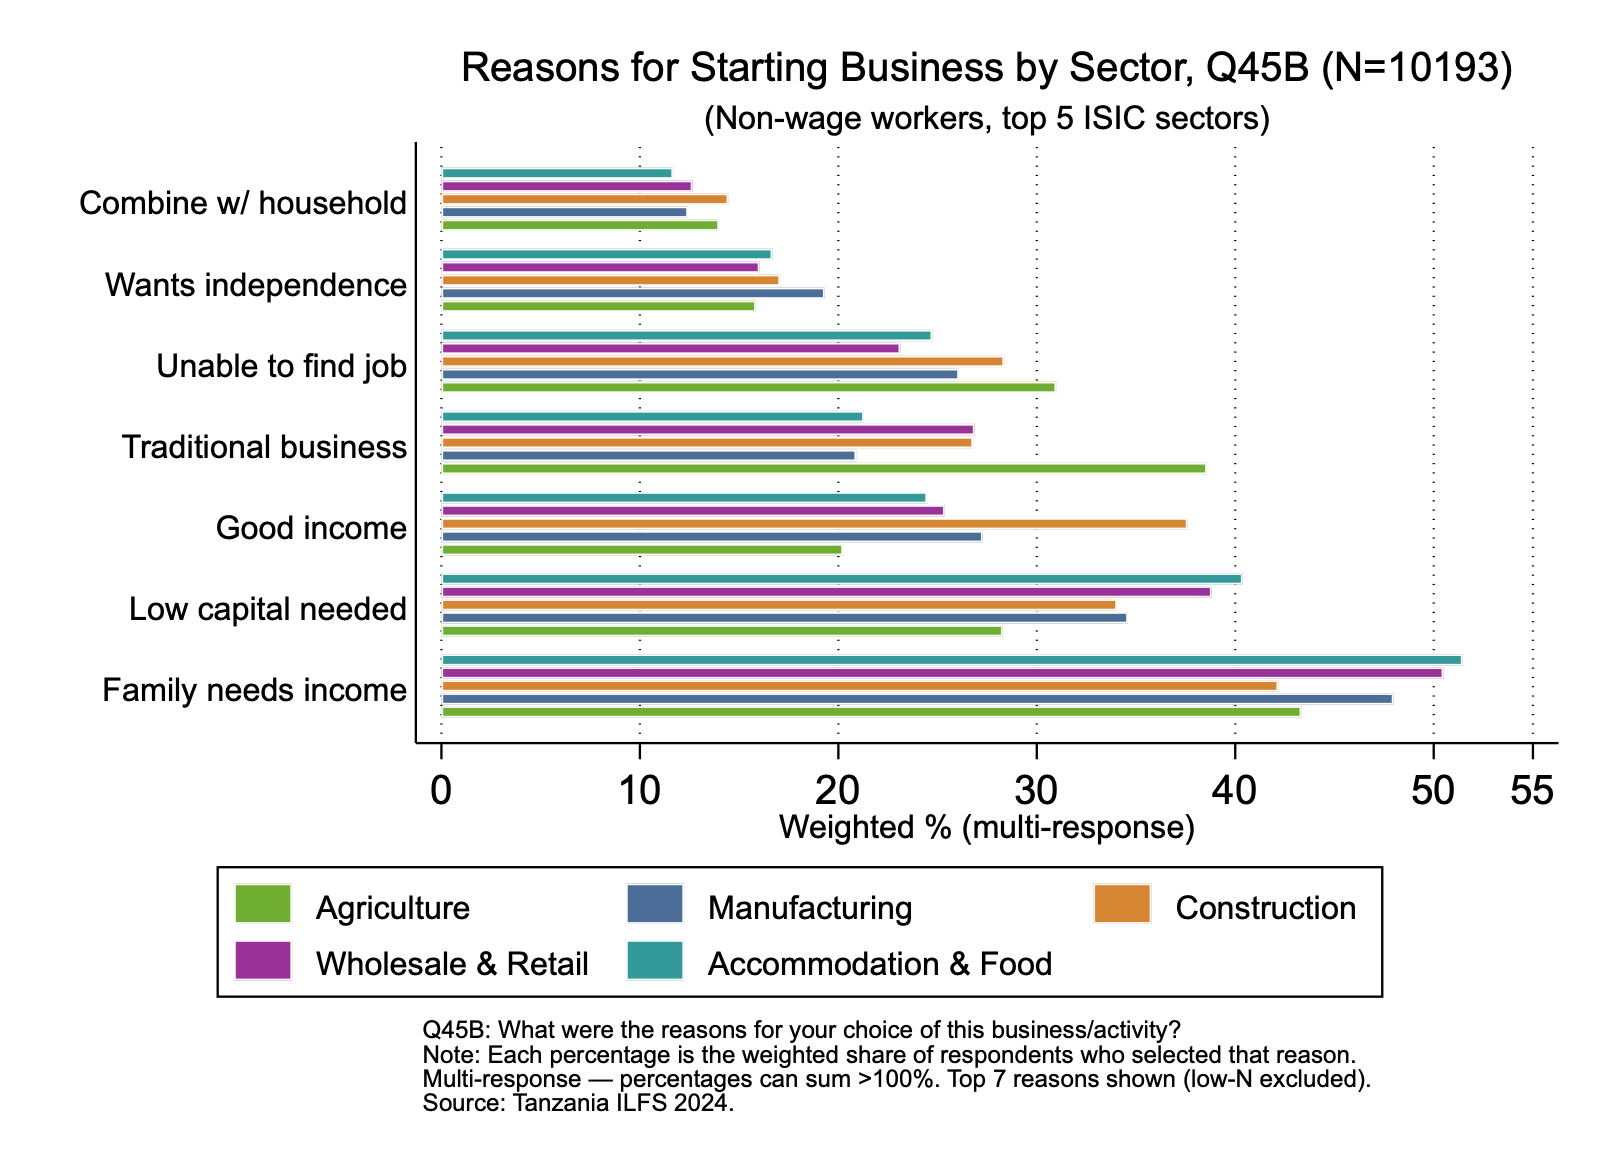
\includegraphics[width=0.9\textwidth]{figures/fig23_q45b_reasons_by_sector.jpg}
  \caption{Reasons for starting a business (Q45B) by sector.}
  \label{fig:q45_reasons}
\end{figure}

Credit access is low overall, ranging from about 2\% to 11\% across sector-gender cells (Figure~\ref{fig:q47a_sector_gender}). The direction of the gender gap varies: in construction women report higher access than men (8.1\% vs 2.4\%), while in accommodation and food services men report higher access (10.7\% vs 8.2\%).

\begin{figure}[H]
  \centering
  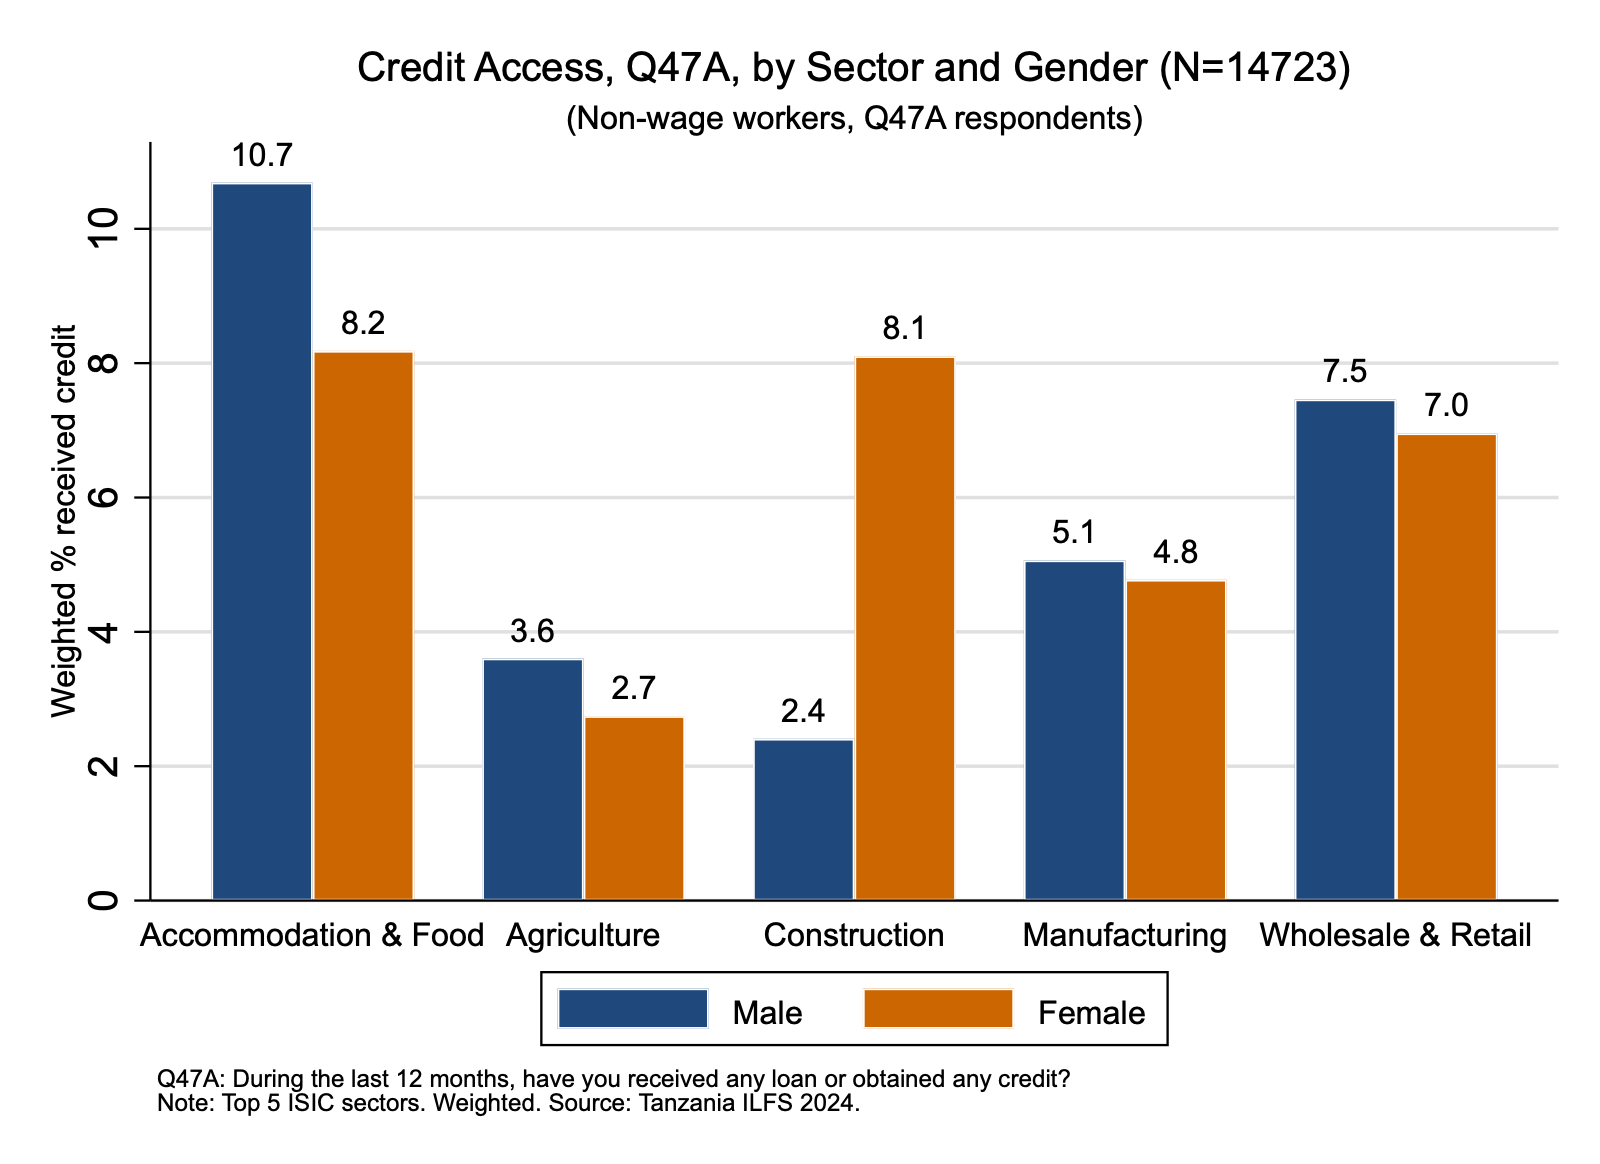
\includegraphics[width=0.85\textwidth]{figures/fig24_q47a_credit_by_sector.jpg}
  \caption{Credit access (Q47A) by sector and gender.}
  \label{fig:q47a_sector_gender}
\end{figure}

The composition of credit sources is also gendered (Figures~\ref{fig:q47b_gender} and~\ref{fig:q47b_sector_gender}). Men more often draw on relatives or friends (24.8\%) and on banks (19.8\%); women more often use SACCOS or VICOBA (22.6\%), private money lenders (18.9\%) and UPATU groups (15.5\%). Sectorally, the same logic recurs: in wholesale and retail women rely heavily on SACCOS or VICOBA (30.6\% vs 18.8\% for men), while agriculture sees both genders drawing on SACCOS and on relatives or friends. Several sector-gender cells are based on small samples.

\begin{figure}[H]
  \centering
  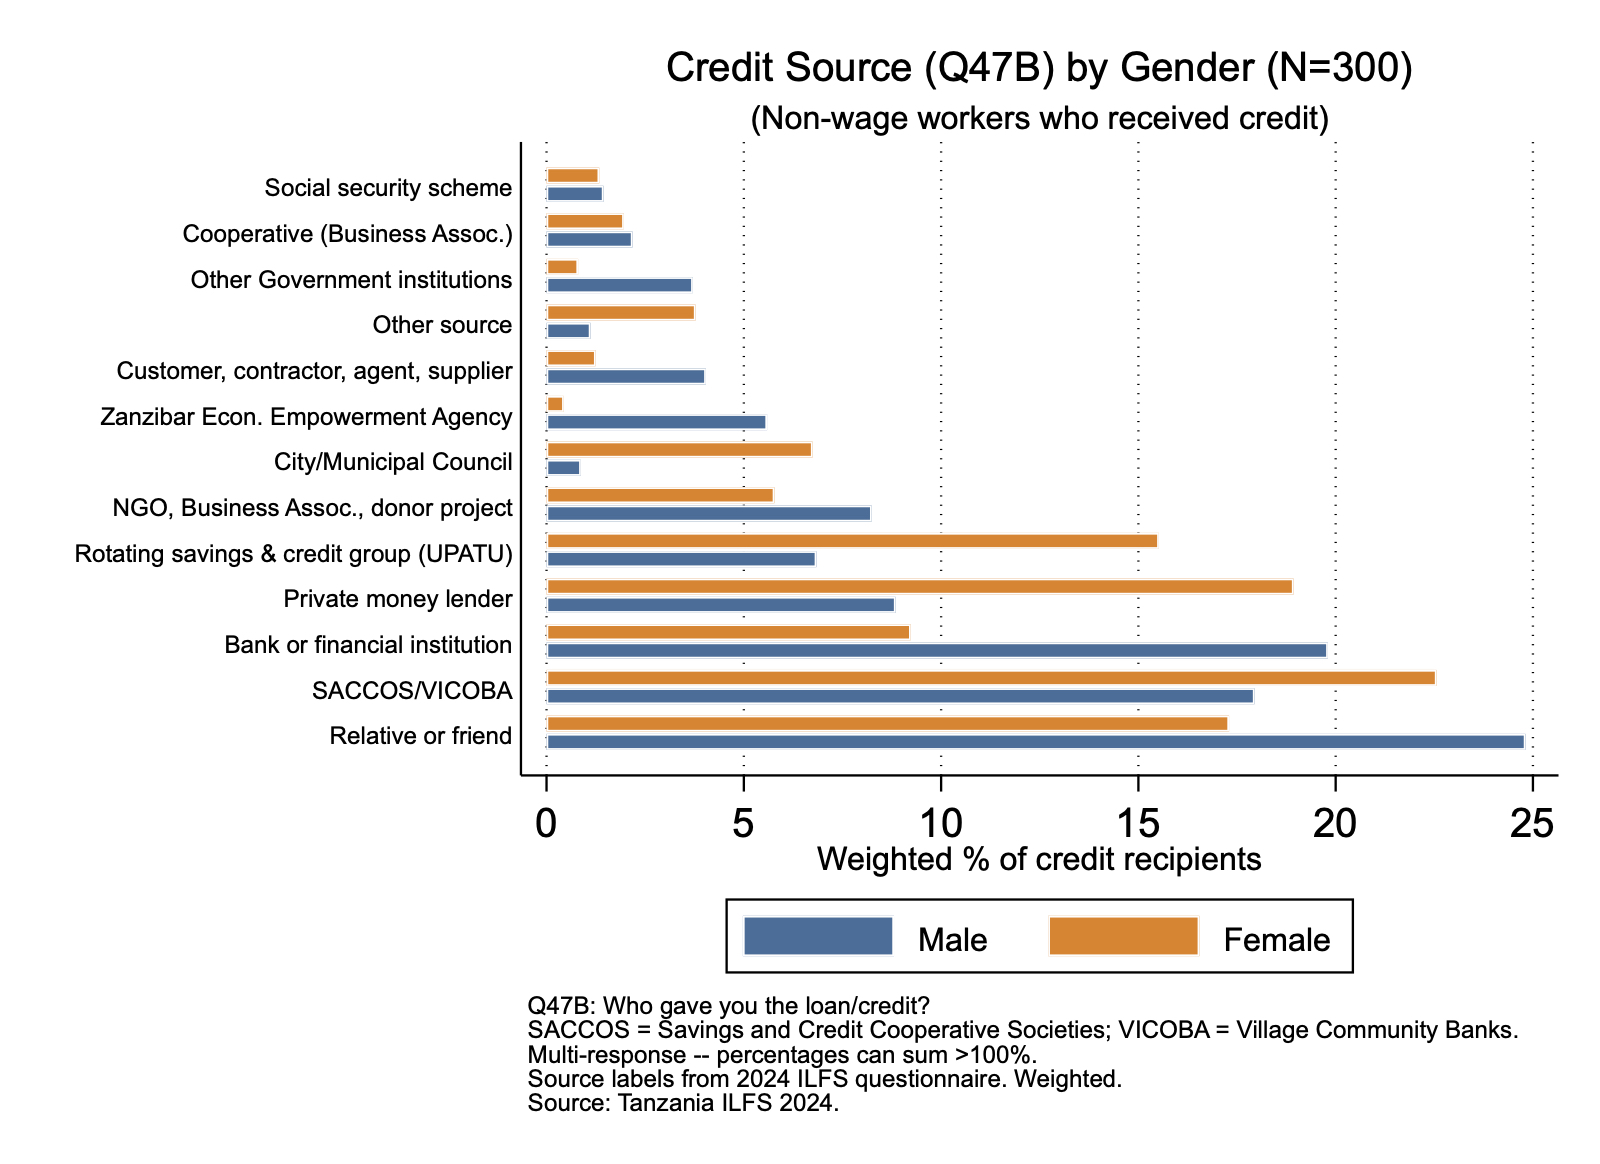
\includegraphics[width=0.9\textwidth]{figures/fig25_q47b_credit_source.jpg}
  \caption{Credit sources (Q47B) by gender.}
  \label{fig:q47b_gender}
\end{figure}

\begin{figure}[H]
  \centering
  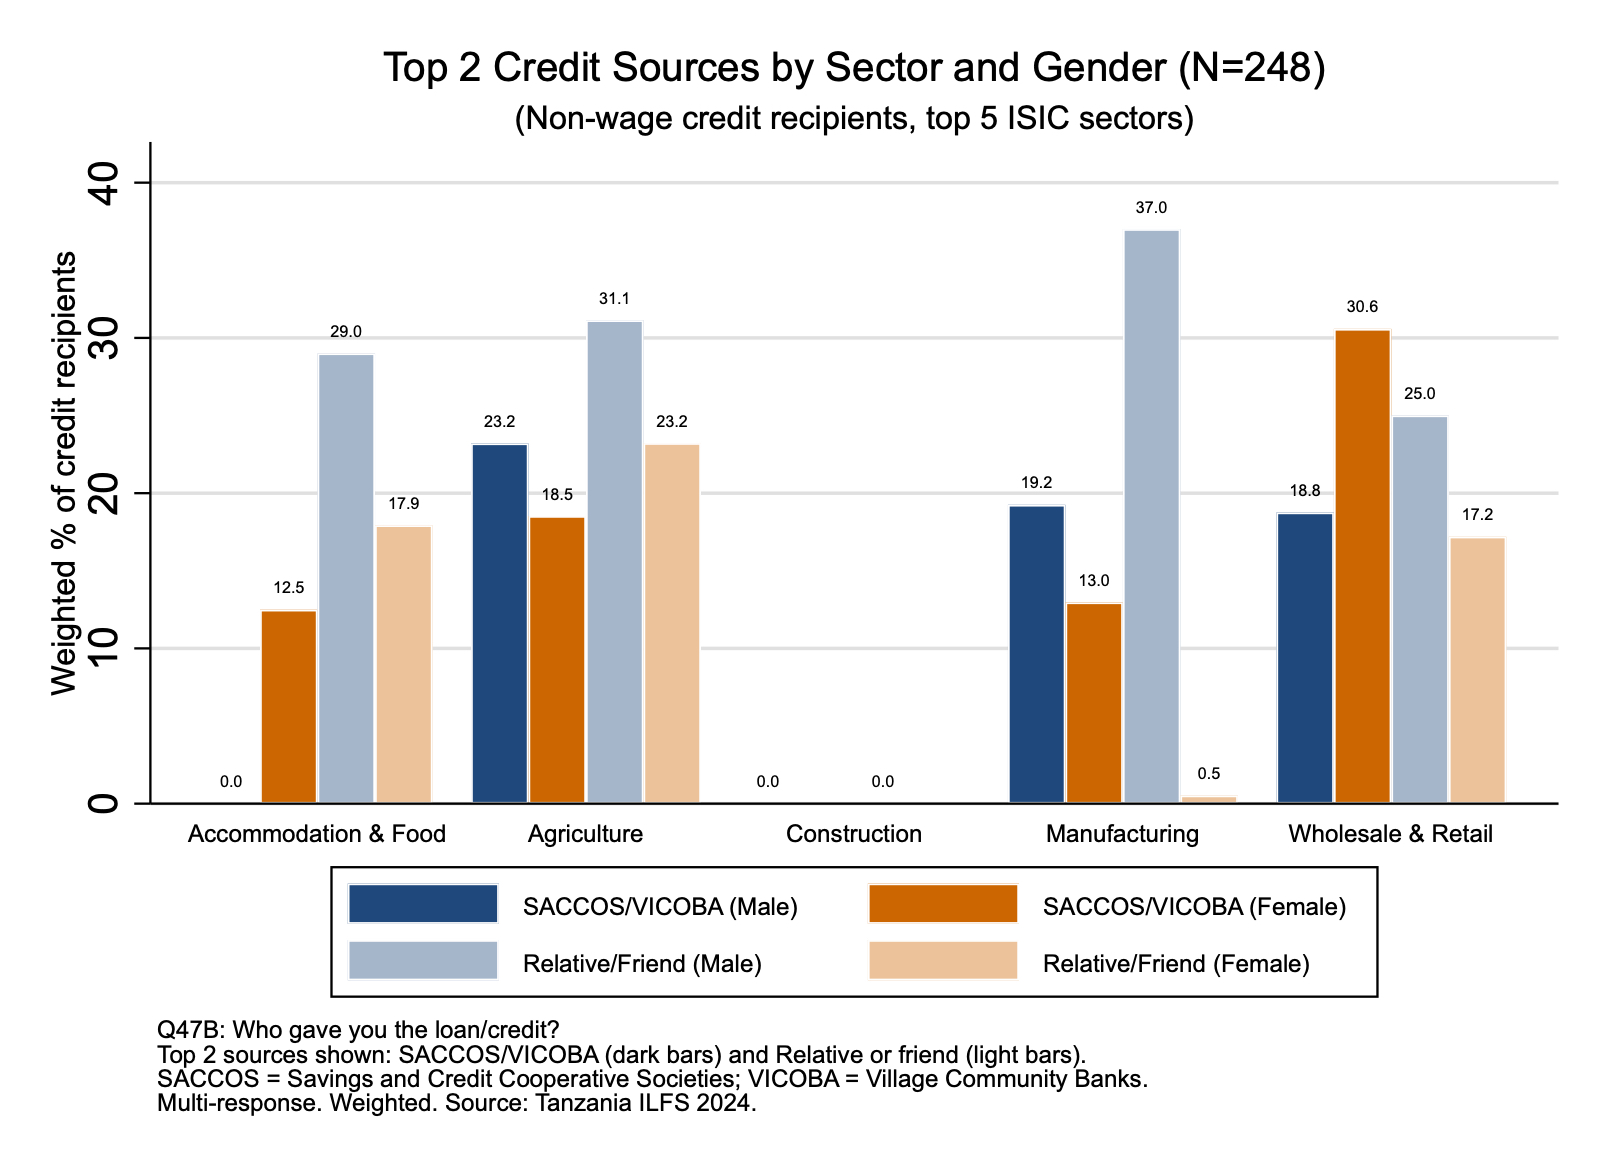
\includegraphics[width=0.9\textwidth]{figures/fig26_q47b_credit_by_sector.jpg}
  \caption{Top credit-source patterns by sector and gender (Q47B).}
  \label{fig:q47b_sector_gender}
\end{figure}


% ══════════════════════════════════════════════════════════
\section{Secondary Activity, Location and Working Time}
\label{sec:location}
% ══════════════════════════════════════════════════════════

\subsection{Secondary economic activity}

Secondary activity is reported by 24.7\% of employed respondents (28.5\% of men and 20.8\% of women) using the combined indicator that flags any of: more than one job last week (Q20), other work for pay or barter last week (Q48A), or a secondary job to which the respondent expected to return (Q48B). The activity-rate version, restricted to workers active in a secondary job in the reference week, is 20.3\% (men 23.6\%, women 16.9\%). Secondary activity is most common among employer informal upper men (43.2\%) and OA upper informal women (38.5\%), and least common among formal wage workers; the gender gap is significant ($p < 0.001$) across most categories (Figure~\ref{fig:secondary_activity}).

\begin{figure}[H]
  \centering
  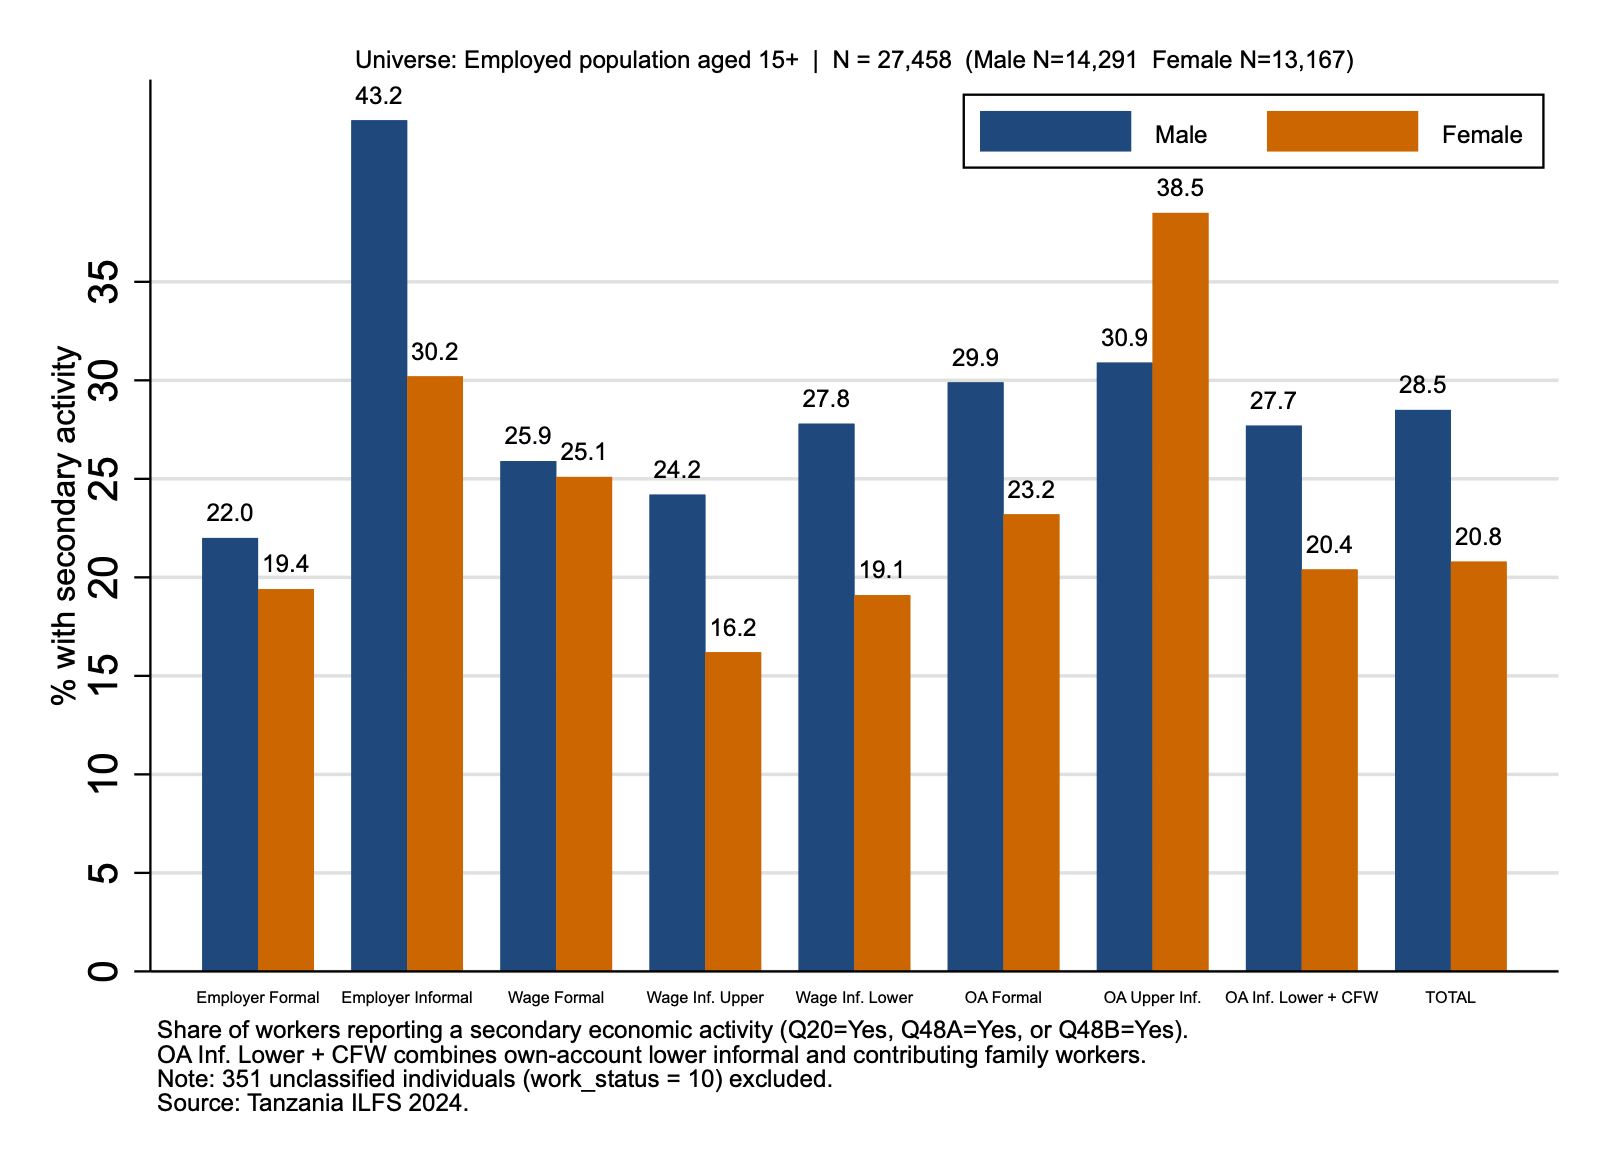
\includegraphics[width=0.9\textwidth]{figures/fig27_secondary_activity.jpg}
  \caption{Secondary economic activity prevalence by work status and gender.}
  \label{fig:secondary_activity}
\end{figure}

\subsection{Labour force status by location}

Splitting the sample into rural districts, other urban areas, and Dar es Salaam shows that the gender gap in employment widens with urbanisation (Figure~\ref{fig:lfs_location}). Male and female employment rates are 89.5\% and 83.2\% in rural areas, 85.0\% and 72.5\% in other urban areas, and 83.4\% and 64.8\% in Dar. The gap therefore expands from 6.3 points in rural areas to 18.6 points in Dar---driven by women shifting into OLF rather than into unemployment as urbanisation increases.

\begin{figure}[H]
  \centering
  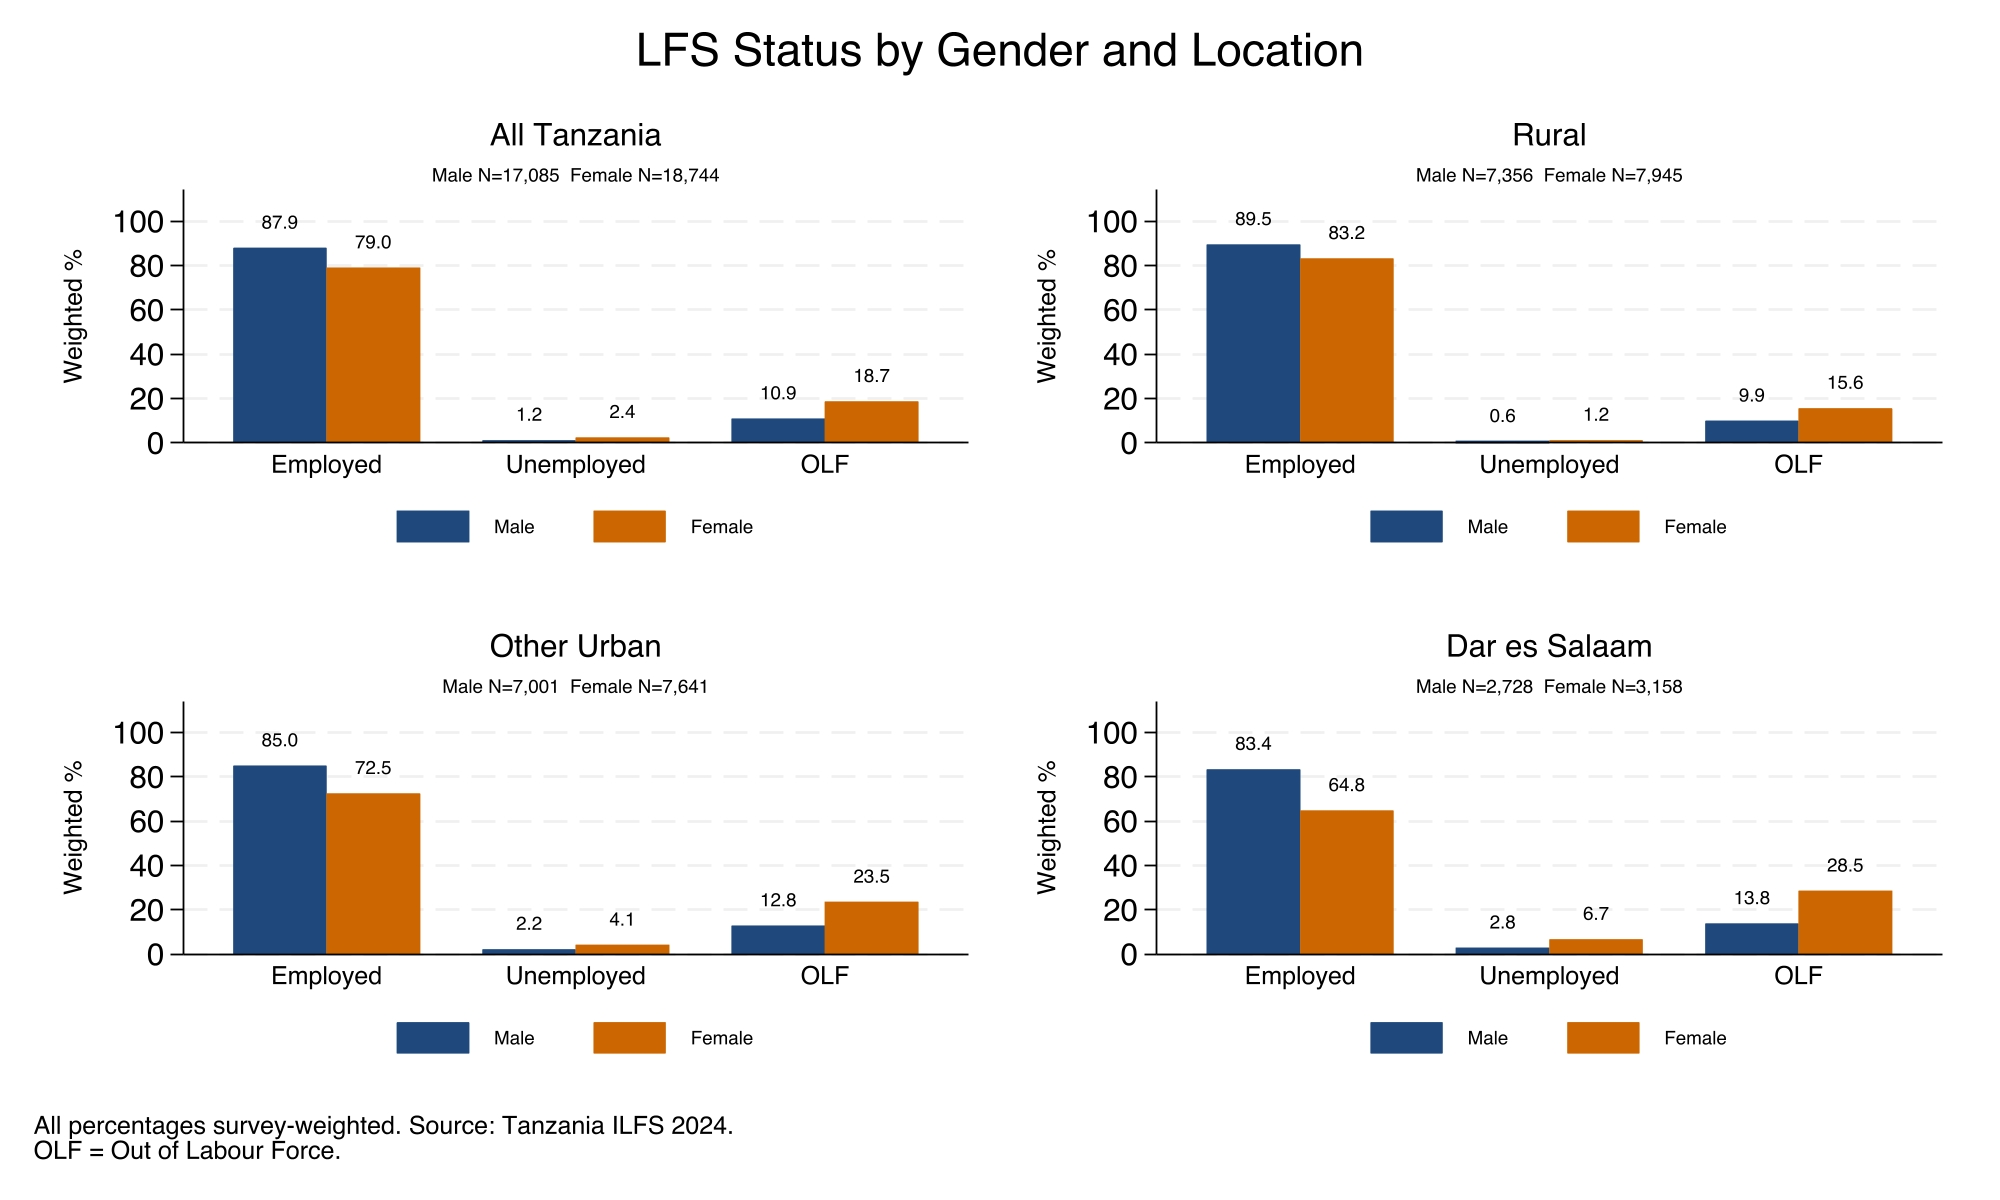
\includegraphics[width=\textwidth]{figures/fig28_lfs_by_gender_location.jpg}
  \caption{Labour force status by gender and location.}
  \label{fig:lfs_location}
\end{figure}

\subsection{Work status by location}

Composition shifts run in parallel (Figure~\ref{fig:ws_location}). In rural districts 81.9\% of employment falls into OA lower informal plus CFW; in Dar the figure is 41.7\%, with the residual taken up mainly by wage formal, wage informal lower and the two upper-informal categories. The female-male gap in OA lower informal plus CFW is 11.2 points in rural areas and 23.2 points in other urban areas: women are more rural-concentrated in the residual category, while urban men diversify out of it more readily than urban women.

\begin{figure}[H]
  \centering
  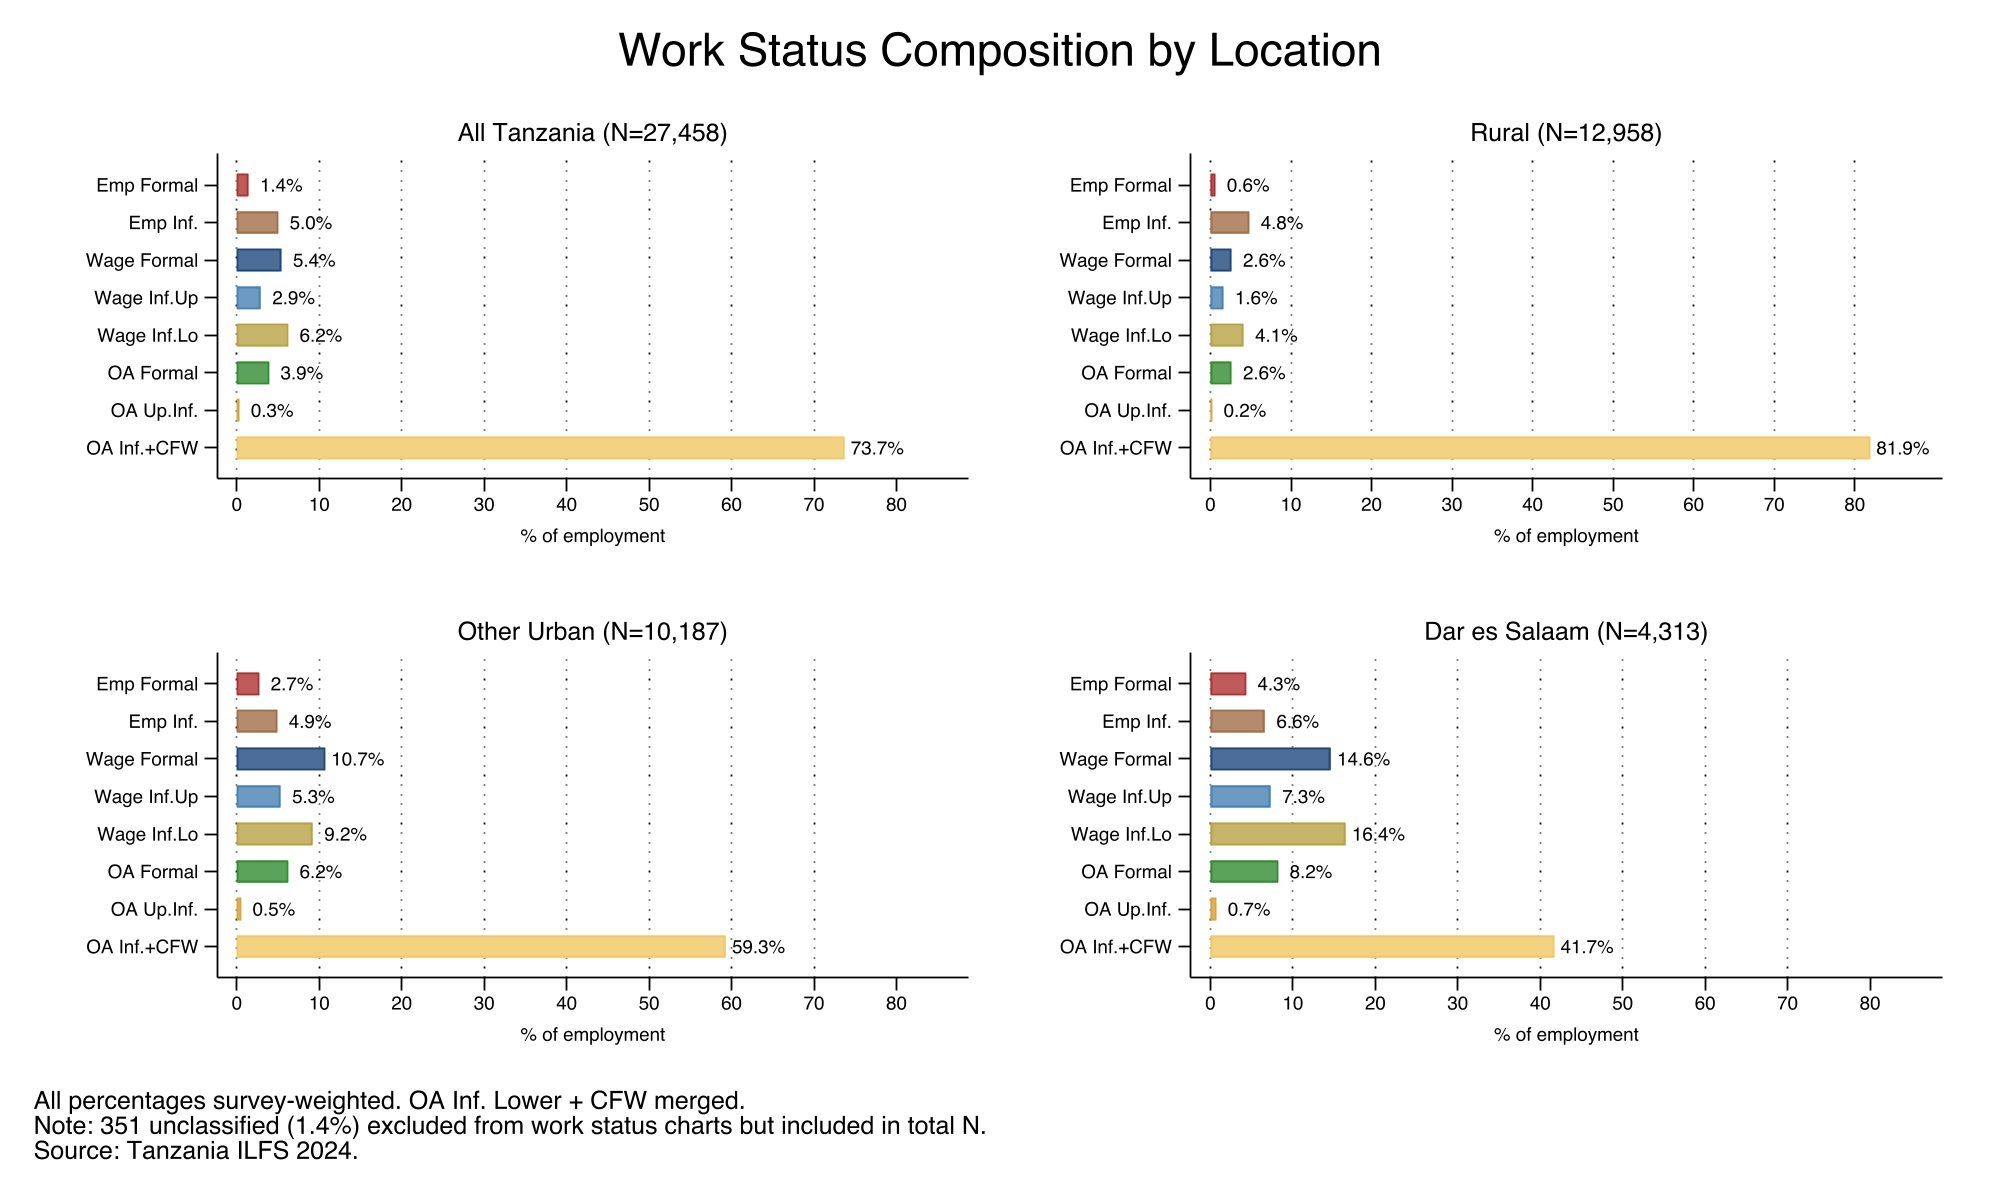
\includegraphics[width=\textwidth]{figures/fig29_work_status_by_location.jpg}
  \caption{Work status composition by location.}
  \label{fig:ws_location}
\end{figure}

\subsection{Online work and working time}

Online work is rare in rural areas (1.5\% for men, 1.1\% for women), higher in other urban areas (7.7\% and 5.5\%) and highest in Dar (12.7\% and 10.8\%) (Figure~\ref{fig:online_location}). The rural-Dar gradient is steeper than the gender gradient at any single location, so geography is a stronger first-order predictor of digital participation than gender.

\begin{figure}[H]
  \centering
  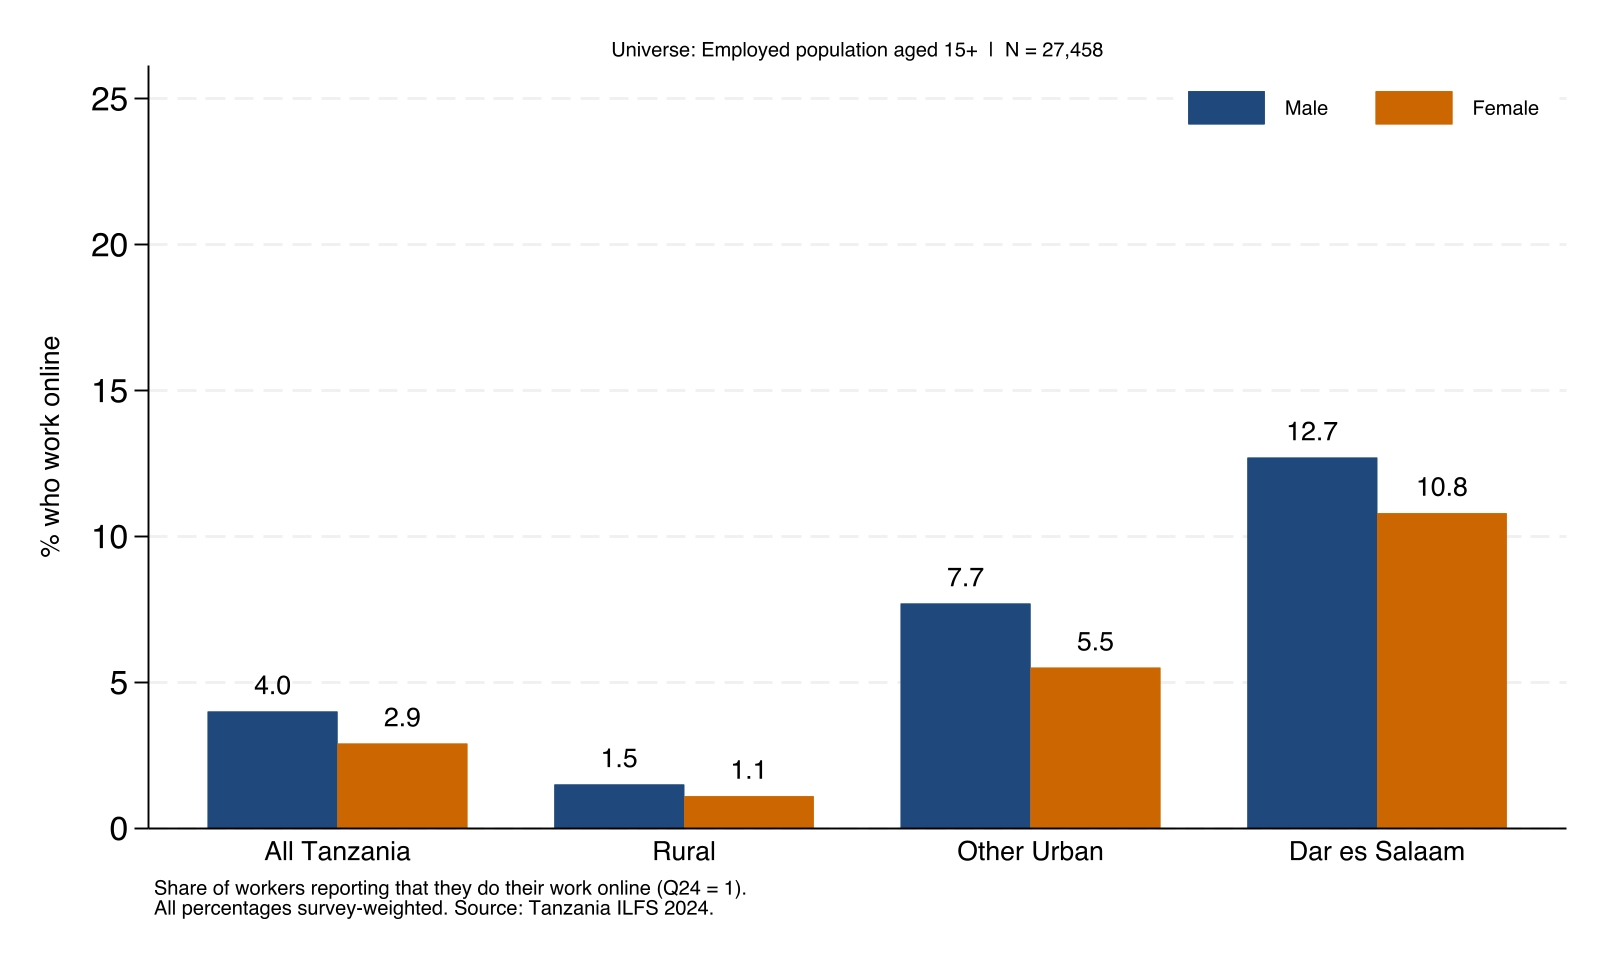
\includegraphics[width=0.9\textwidth]{figures/fig30_online_work_by_location.jpg}
  \caption{Online work by gender and location.}
  \label{fig:online_location}
\end{figure}

Working time displays a clear seasonal pattern (Figure~\ref{fig:hours_location_qtr}). Mean weekly hours peak in the first quarter (about 61 hours for men) and fall to 48--50 hours in Q2--Q3 before partial recovery in Q4. Rural areas show the sharpest within-year swing, consistent with the agricultural calendar; Dar shows the flattest profile.

\begin{figure}[H]
  \centering
  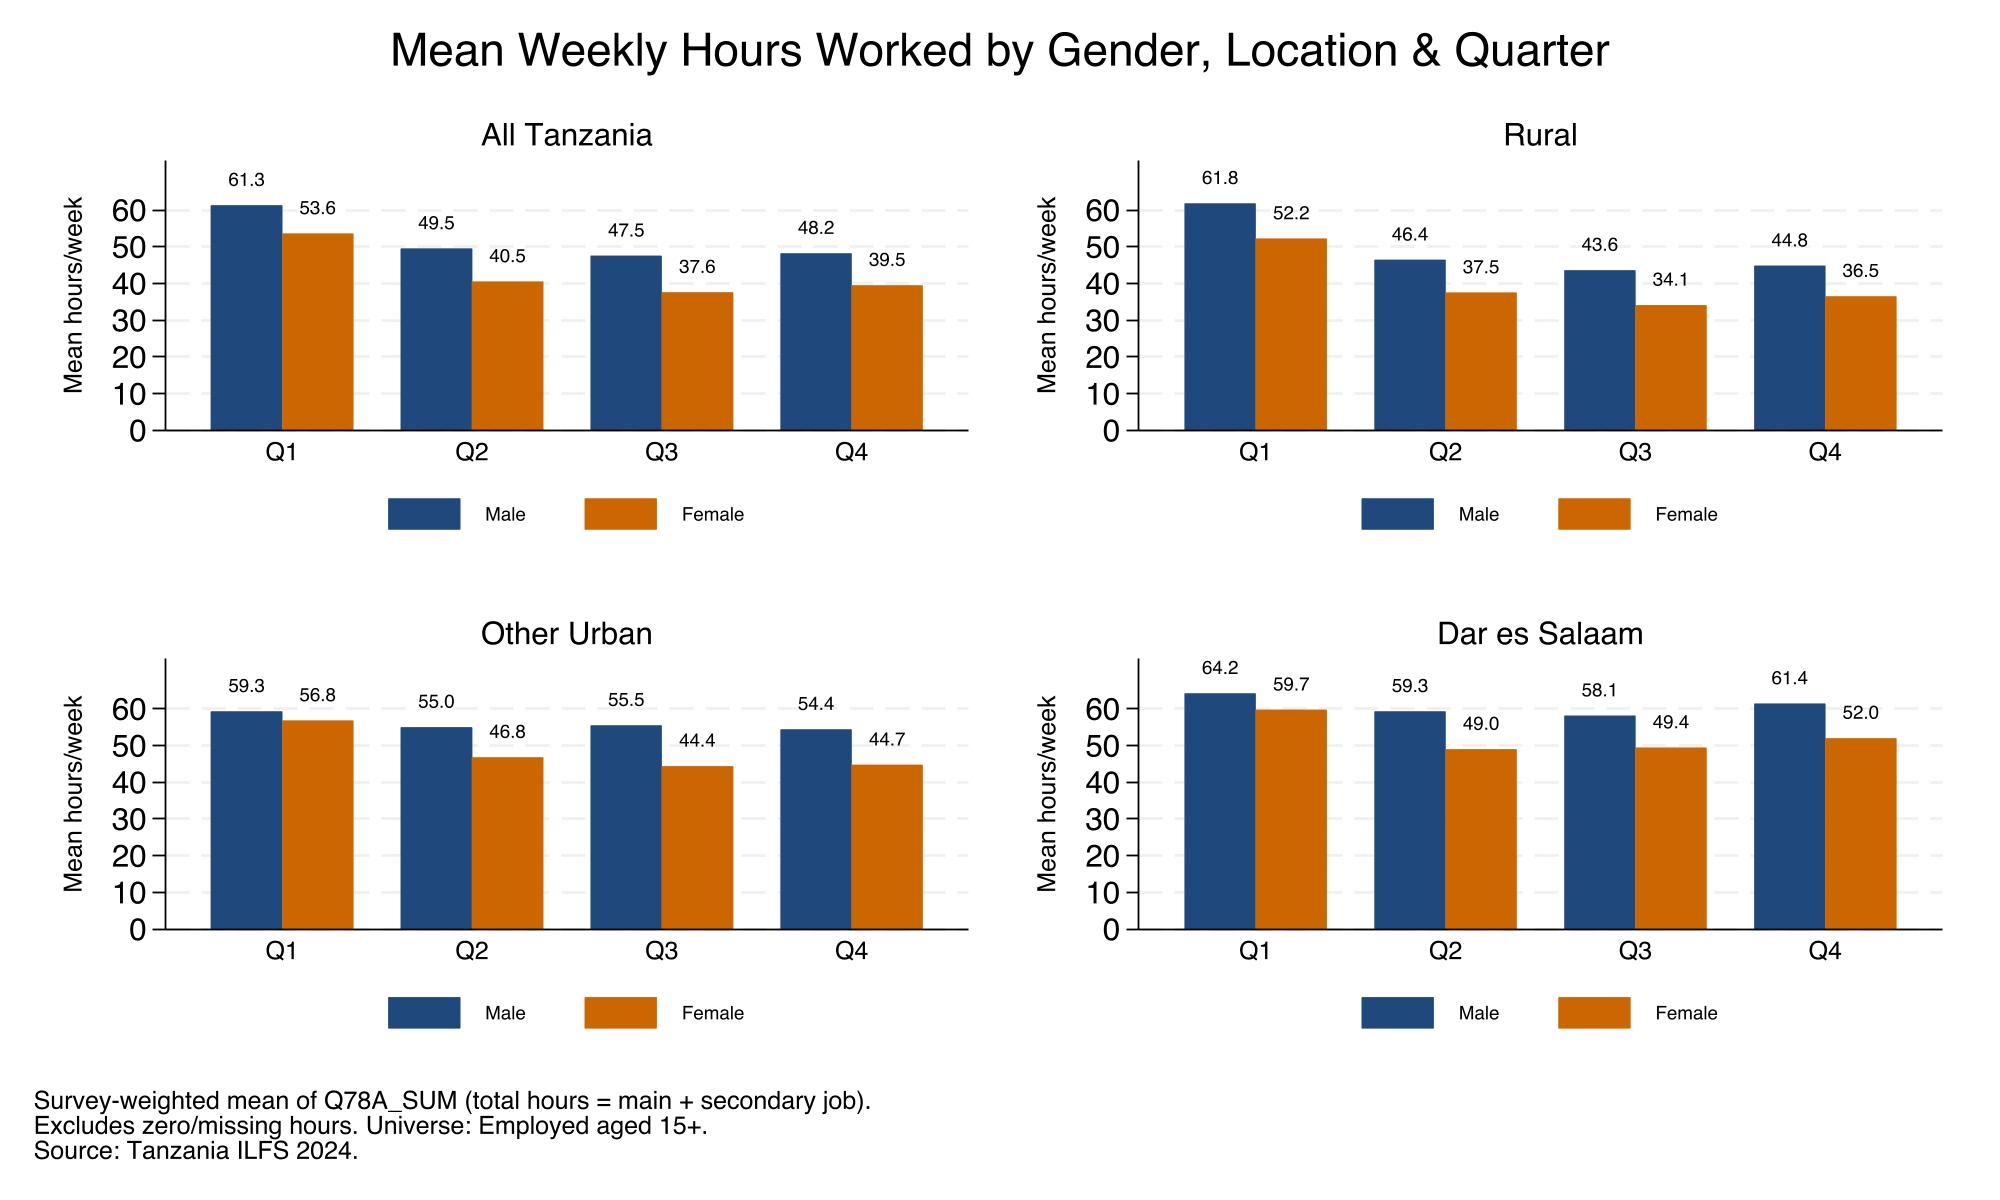
\includegraphics[width=\textwidth]{figures/fig31_hours_by_location_quarter.jpg}
  \caption{Mean weekly hours worked by gender, location and quarter.}
  \label{fig:hours_location_qtr}
\end{figure}


% ══════════════════════════════════════════════════════════
\section{Conclusion}
\label{sec:conclusion}
% ══════════════════════════════════════════════════════════

The 2024 ILFS describes a labour market that combines high participation with a job mix dominated by lower-tier informal own-account work and contributing family workers. The aggregate employment rate of 83.2\% is consistent with previous rounds, but the share of formal wage employment (5.4\%) is small and the share of OA lower informal plus CFW (73.7\%) is large.

Gender, age, education, sector and location each modulate the same underlying composition. Women are concentrated in OA lower informal and CFW, and the gap relative to men widens as one moves from rural areas to Dar. Care-related responsibilities, visible in the OLF distribution, account for most of the gender gap in participation. Education sorts workers into segments early; among employed youth, the OA lower informal plus CFW share is even larger than among adults. The education profiles of higher-tier categories are roughly comparable across genders for wage formal jobs but diverge sharply for OA upper informal, where women hold far less human capital than men.

Sectoral and sub-sectoral views show that informality is structural, not residual. Agriculture is overwhelmingly lower-tier informal, manufacturing is dominated by labour-intensive sub-sectors with high female shares and low formality, and only public administration and education approach majority formal employment. Construction is unusual in carrying both a large upper-informal segment and a stronger ``good income'' motive in the enterprise module.

Enterprise-level patterns reinforce these conclusions. Most informal businesses are entered out of necessity or because start-up capital is low. Credit access is limited (2--11\% across sector-gender cells), and the composition of credit sources is gendered, with women relying more on SACCOS, VICOBA and UPATU groups and men more on relatives, friends and banks. Secondary activity is widespread among lower-tier and upper-informal workers and rare among formal wage workers, reinforcing the picture of multiple, partial sources of income outside the formal segment.

The location and time-use diagnostics introduce a further layer. The participation gender gap, the work-status mix and the prevalence of online work all vary substantially across rural, other urban and Dar es Salaam contexts, while working time follows a marked agricultural calendar. Diagnostics that average across geographies or quarters are likely to understate both the spatial unevenness of formal-sector access and the seasonal swings in labour intensity.


% ══════════════════════════════════════════════════════════
\section*{Methodological Note}
\addcontentsline{toc}{section}{Methodological Note}
% ══════════════════════════════════════════════════════════

\textbf{Survey.} Tanzania Integrated Labour Force Survey 2024. All percentages are survey-weighted (variable WEIGHT) using \texttt{svy: proportion} and \texttt{svy: mean} in Stata.

\textbf{Universe.} Working-age population aged 15 and above, $N = 35{,}829$ (population of about 37.3 million). Employed sub-sample: $N = 27{,}458$ (about 31.0 million).

\textbf{Employment definition.} ILO 13th ICLS. Employed if any of: Q13A in 1--7 (productive activity last week); Q13C=1 (paid work); Q13D=1 (business); Q13E=1 (helped a family member's paid work); Q14A or Q14B=1 (absent but has a job); Q14G in 1--4 (absent, farming or fishing).

\textbf{Work status classification.} The pipeline constructs a ten-category status variable aligned with ILO ICSE-93 (with Q34 social security reinstated for wage formality and Q21B occupation codes 1--4 used to identify the upper-tier informal segments). Sections~\ref{sec:work_status}--\ref{sec:educ_formal} use an eight-category display in which OA lower informal and CFW are merged for legibility. Sections~\ref{sec:sectors} and~\ref{sec:informal_credit} use the underlying ten-category variable with selective merges as described in each figure caption.

\textbf{Geographic disaggregation.} Three areas: rural (district councils), other urban (town, municipal and city councils outside Dar), and Dar es Salaam (REGION = 7).

\vspace{1em}
\noindent\textbf{Client:} FCDO / ODI \hfill \textbf{Prepared by:} Tomoto Masuda \hfill \textbf{Date:} 22 March 2026


% ══════════════════════════════════════════════════════════
\newpage
\bibliographystyle{apalike}
\bibliography{references_Tanzania_ilfs_2024}
% ══════════════════════════════════════════════════════════

\end{document}
